% ============================================================
% 中文论文模板 - 基于 ctexart 文档类
% 编译器：必须使用 XeLaTeX
% ============================================================

\documentclass[UTF8, zihao=5,AutoFakeBold=2]{ctexart}  
% UTF8: 编码格式；zihao=5: 设置正文字号为五号（10.5pt）

% ============================================================
% 页面设置（使用 geometry 宏包）
% ============================================================
\usepackage[top=2.54cm, bottom=2.54cm, left=3.18cm, right=3.18cm]{geometry}
\setlength{\intextsep}{5pt}
% ============================================================
% 颜色与超链接
% ============================================================
\usepackage[colorlinks, linkcolor=blue, citecolor=green, urlcolor=red]{hyperref}

% ============================================================
% 图片与表格
% ============================================================
\usepackage{graphicx}      % 插入图片
\usepackage{float}         % 控制浮动体位置（H 选项）
\usepackage[section]{placeins} % 防止图表跨节浮动
\usepackage{subcaption}    % 子图
\usepackage{booktabs}      % 三线表（学术表格）
\usepackage{array}         % 增强表格功能
\usepackage{longtable}     % 跨页长表格
\usepackage{multirow}      % 合并单元格

% ============================================================
% 数学公式
% ============================================================
\usepackage{amsmath}       % 数学公式增强
\usepackage{amssymb}       % 数学符号
\usepackage{bm}            % 加粗数学符号

% ============================================================
% 其他常用宏包
% ============================================================
\usepackage{fancyhdr}      % 页眉页脚自定义
\usepackage{indentfirst}   % 首段缩进（中文习惯）
\usepackage{enumitem}      % 列表定制
%\usepackage{enumerate}
\usepackage{wrapfig}
\usepackage{caption}       % 标题定制
\captionsetup{font=small}   % 图表标题字体统一略小
\usepackage{cite}  % 配合手写 thebibliography 使用 \cite
% 说明：本文采用手写 thebibliography + cite 宏包。


% ============================================================
% 数模竞赛常用宏包
% ============================================================
\usepackage[ruled, linesnumbered]{algorithm2e}  % 算法/伪代码
\usepackage{listings}                            % 代码排版
\lstset{
    basicstyle=\small\ttfamily,
    breaklines=true,
    breakatwhitespace=false,
    breakindent=0pt,
    columns=flexible,
    xleftmargin=0pt,
    xrightmargin=0pt,
    frame=none,
    numbers=none,
    aboveskip=6pt,
    belowskip=6pt
}
% ---------- 附录代码块字体：拉丁用 DejaVu 等宽、中文用 Noto 等宽 ----------
% 代码块里的希腊字母、≤、√、±、m² 在 Latin Modern Mono 里没有字形，换成 DejaVu 等宽；
% 中文改走 Noto 等宽。两个比例尺由 build_appendix.py 按最宽的一行代码反推：拉丁等宽字符
% 宽 0.602 em，中文全角宽 1 em，所以中文取 1.204 倍，一个汉字正好两个半角位，中英混排的
% 注释才对得齐。正文里的等宽字不受影响。
\newfontfamily\codefont{DejaVu Sans Mono}[Scale=0.666]
\setCJKfamilyfont{zhcode}{Noto Sans Mono CJK SC}[Scale=0.802]
\newcommand{\codefamily}{\codefont\CJKfamily{zhcode}}
% 圈数字 ① 到 ⑦ 交给中文字体，DejaVu 等宽里没有这几个字形
\xeCJKDeclareCharClass{CJK}{"2460 -> "2473}
\lstset{
    % 代码段落的中文行距会被 ctex 拉到 1.56 倍，附录三千多行按那个行距要多出二十几页，
    % 这里压到 0.85，一行 9.2 pt，汉字行高 1.27 倍，不挤也不散
    basicstyle=\linespread{0.85}\selectfont\small\codefamily,
    language=Python,
    keywordstyle=\color{blue!70!black},
    commentstyle=\color{green!45!black},
    stringstyle=\color{red!60!black}
}
% ---------- 附录代码块字体结束 ----------
\usepackage{tikz}                                % 流程图/示意图
\usetikzlibrary{arrows.meta, positioning, shapes.geometric}

% ============================================================
% 页眉页脚设置
% ============================================================
\pagestyle{fancy}
\fancyhf{}
\fancyfoot[C]{\thepage}    % 页脚居中显示页码
\renewcommand{\headrulewidth}{0.4pt}  % 页眉横线

% ============================================================
% 标题格式设置
% ============================================================
\ctexset{
    section/format={\heiti\centering\zihao{3}\bfseries},        % 一级标题：三号加粗居中
    subsection/format={\heiti\zihao{-4}\bfseries},        % 二级标题：小四加粗
    subsubsection/format={\heiti\zihao{5}\bfseries},        % 三级标题：五号加粗
    paragraph/format={\zihao{-5}\bfseries},
}

% ============================================================
% 文档开始
% ============================================================
\raggedbottom
\begin{document}
% ---------- 标题 ----------
\newpage

	{\centering
	{\zihao{2}\bfseries 无线电干扰源的快速自动定位与清除的研究} \\[0.5cm]
	% ---------- 摘要 ----------

	\section*{摘要}
	\addcontentsline{toc}{section}{摘要}

	}

	随着无线电通信技术的飞速发展，频谱资源日益紧张，在危险环境中人工排查干扰源面临极大挑战。我们针对搭载于机器狗的干扰源自动定位与清除系统，综合运用\textbf{计算几何}、\textbf{\textit{Fisher}}\textbf{信息论}与\textbf{路径规划}理论，建立了一套确定性的搜索、定位与清除数学模型，实现了对区域内全向及定向干扰源的\textbf{高效排查与清除}。

\textbf{针对问题一}：需要计算交会定位区域的直径并判断直径圆能否覆盖该区域。通过建立\textbf{楔形约束模型}并近似为三角形，利用凸集性质证明交集为凸多边形 \(\Omega\)，将直径计算转化为\textbf{顶点对最大距离问题}，提出以直径中点为圆心、\(D/2\) 为半径的圆覆盖判定准则。仿真算例表明，该算法能精确算出定位区域直径（4点交会时 \textbf{\(D \approx 28.632m\)}），并有效判别覆盖性。

\textbf{针对问题二}：需要确定第二检测点的选择策略及候选区域。利用\textbf{Fisher信息矩阵}证明已知距离时\textbf{最优交会角恒为} \textbf{\(90^{\circ}\)}，针对源位置与距离均未知的情况，提出“保证交会角”与“最小最坏直径”\textbf{两条稳健准则}，构造出透镜形可行域 \(\mathcal{F}\)。求解得到最优点\textbf{距第一点约} \textbf{\(1004\text{m}\)}，交会角介于 \textbf{\(36.2^{\circ} \sim 39.6^{\circ}\)} 之间，最坏定位直径约 \textbf{\(134.1\text{m} \sim 134.8\text{m}\)}，候选区域面积约 \textbf{\(0.021\text{km}^2\)}。
  

\textbf{针对问题三}：需要在源位置与数量均未知的圆域内，规划机器狗以最短时间完成全向干扰源的搜索、定位与清除。首先，我们将检测问题转化为\textbf{“7个半径1000m的圆覆盖半径1800m圆域”}的几何覆盖问题；其次，设计\textbf{确定性两阶段策略}：阶段一进行起点全频道扫描与布局定向，基于\textbf{Held-Karp算法}求解巡视最短开放路径，并引入“够准即停”裁剪与基于方位扇区的\textbf{顺路清除模型}；阶段二对剩余目标采用\textbf{“就近试清\(\to\)多点覆盖试清\(\to\)文献准则补测\(\to\)末端逼近”四级递进清除机制}。仿真结果表明，三次正式模拟分别清除 \textbf{14}、\textbf{15}、\textbf{16} 个干扰源，虚拟总耗时分别为 \textbf{3722.4}、\textbf{3126.4}、\textbf{4058.8\,s}，平均定位清除时间分别为 \textbf{265.9}、\textbf{208.4}、\textbf{253.7\,s/个}，三次平均虚拟总耗时 \textbf{3635.9\,s}。


\textbf{针对问题四}：需要解决定向源“背光侧返回no\_signal”导致原检测策略失效、且no\_signal无法作为定位硬约束的问题。为此，我们建立\textbf{“半圆盘命中模型”}刻画定向源的波束覆盖特性，并提出\textbf{“原点+7基点+12外圈点（半径1850m）”的20点定案布局}；在定位阶段，仅使用direction与near两类硬约束进行交会；清除阶段采用\textbf{“顺路清除\(\to\)就近试清\(\to\)兜底逼近”三级递进机制}，其中顺路清除引入基于最小覆盖圆（MEC）圆心与贪心覆盖圆的清除动作。仿真结果表明，三次正式模拟分别清除 \textbf{16}、\textbf{13}、\textbf{10} 个干扰源，虚拟总耗时分别为 \textbf{6406.0}、\textbf{6809.1}、\textbf{6503.3s}，平均定位清除时间分别为 \textbf{400.4}、\textbf{523.8}、\textbf{650.3s}，三次平均虚拟总耗时 \textbf{6572.8s}。

	\vspace{1cm}
	{\heiti 关键词：}示向度交会定位；Fisher 信息矩阵；稳健布站；圆覆盖布局；Held-Karp 路径规划；顺路清除；半圆盘命中模型

\newpage
% ---------- 正文开始 ----------
\section*{一、 问题综述}
	\subsection*{1.1问题背景}
	随着无线电通信技术的飞速发展，频谱资源日益紧张，各类无线电干扰源数量激增。在危险环境（如化工厂、核辐射区）中，传统的人工徒步排查方式不仅效率低下，更严重威胁技术人员的人身安全。而将干扰源自动定位与清除系统搭载于机器狗上，可以有效地替代人类在危险环境中完成对干扰源的定位以及清除工作，以满足频谱管理领域的迫切需求。
	
	本文针对搭载于机器狗的干扰源自动定位清除的智能系统在未知环境中开展排查任务这一情景，在圆形目标区域边界、测向机工作方式、干扰源覆盖特性及初始坐标等条件已经明确的情况下，需要综合建立干扰源示向度交会定位的几何模型与信号场强衰减模型，并对机器狗的自主搜索、精准定位及清除策略进行路径与时间的协同优化，以达到在确保所有干扰源被清除的前提下任务完成时间最短这一目标。
	
	\subsection*{1.2问题重述}
	
		问题一:\quad 已知若干检测点坐标及示向度，计算交会定位区域直径，并判断以该直径为直径的圆能否覆盖定位区域。
		
		问题二:\quad 已知某全向干扰源在一检测点的示向度，为确保获得的定位效果较好，确定第二个检测点的选择策略及候选区域。
		
		问题三:\quad 机器狗从原点出发自动定位清除10\textasciitilde16个全向干扰源，要求在确保所有干扰源被清除的前提下,求使清除总时间最短的策略与算法。
		
		问题四:\quad 在第三问的前提下，目标区域增加了全向与定向干扰源，两者共存总数在10\textasciitilde16个之间且具体个数均未知，定向干扰源的定向方向也未知，需制定检测清除策略并通过模拟器验证。

\section*{二、 模型建立}
	\subsection*{问题一:交会定位法定位区域直径的计算与覆盖判定}
	干扰源必落在各检测点示向度±1°张开的楔形内，先建立单检测点的楔形约束模型，再增加其他检测点，自圆域起依次与各楔形做半平面裁剪求交。由凸几何性质确定定位区域为凸多边形，从而得出直径取任意两顶点的距离最大值。并记下达到直径的端点，以该直径线段为直径作圆，判断区域顶点是否全部落在圆内，即可回答能否覆盖。
    
	\subsection*{问题二:第二检测点选择策略及候选区域确定}
	对于问题二而言，在某全向干扰源已由第一个检测点\(S_1\)测得示向度\(\theta_1\)的条件下，需要确定第二检测点\(S_2\)的选择策略。求解的关键基于以下三大事实：
    \begin{enumerate}[label=(\arabic*)]
        \item 单点不可定位：单点仅能确定射线，距离\(d_1\)完全不可观测，必须引入第二检测点；
        \item 误差逐点位固定：同一地点的电磁环境干扰固定，重复检测不改变误差，因此\(S_2\)必须是一个真正的独立新地点；
        \item 源的位置与距离均未知：仅知真实方位角落在\(\theta_1\pm1^\circ\)、\(d_1\in(5,1500]\)，故源的不确定集是二维的，策略须对其内任一点稳健有效。
    \end{enumerate}
    求解路线：在\(S_1\)建立局部坐标系，利用Fisher信息矩阵（FIM）刻画定位不确定性，借助框架理论给出已知距离时的最优交会几何（\(\phi=90^\circ\)）；将其转化为交会定位区域直径；针对源位置与距离均未知，按有效接收半径下界\(1000\) m作最坏情形稳健设计，并以“最坏直径不超过最优值\(1+\eta\)倍”划定\(S_2\)候选区域。
    
	\subsection*{问题三:全向干扰源自动搜索定位与清除策略}
	该目标区域中的干扰源均为全向干扰源，总共有 10-16 个，但具体个数未知。现机器狗从原点出发，测向机初始频道为 1，对目标区域干扰源进行自动定位并清除。要求在确保所有干扰源被清除的前提下，完成任务的时间越短越好。需要我们制定机器狗自动搜索定位及清除的策略，并设计相应的算法。本题要求机器狗从原点出发，清除目标区域内数量未知的全向干扰源。由于干扰源的有效接收半径 \(R_G \in [1000,1500]\) 存在不确定性，为保证检测的鲁棒性，采取保守策略：只要机器狗与干扰源的距离 \(|SG| \le 1000\)，即可确保成功检测。

由此，问题核心转化为：如何选取最少的检测点，使得以这些检测点为圆心、半径 \(1000\) 的圆能够完全覆盖半径为 \(1800\) 的目标区域。该问题本质上是经典的几何圆覆盖问题。经分析，最少需要 \(7\) 个检测点（即 \(7\) 个半径 \(1000\) 的圆）方可完全覆盖。

	\subsection*{问题四:多类型干扰源检测与清除策略及模拟验证}
问题四引入了定向干扰源。这类源只在波束角 \(\pm 90^{\circ}\)（全角 \(180^{\circ}\)）的范围内发射信号，一旦机器狗处于它的背光侧，接口就会返回 \texttt{no\_signal}。

这个物理特性直接导致我们在问题三中使用的策略无法继续套用，具体表现在以下两方面：


    检测上存在盲区：问题三设计的 7 点覆盖，原本是为了确保“圆域内任意点到最近巡视点 \(\leq 1000\text{m}\)”，只要距离够近，全向源就一定能被听到。但面对定向源，如果机器狗恰好站在它的背面，哪怕距离再近也听不到任何声音（我们通过实测发现，7 点布局对定向源的听到率仅有 \(80.7\%\)）。这意味着原来的覆盖布局不再能保证“一定能听到”。
    定位逻辑失效：在问题三中，我们把 \texttt{no\_signal} 当做“源在检测点 \(1000\text{m}\) 之外”的定位硬约束，用来缩小搜索范围。但现在，\texttt{no\_signal} 可能仅仅是因为“方向没对准”，因此不能再粗暴地把它转化为“源在圆盘外部”的几何约束。
面对这个变化，我们需要在源位置、波束方向以及接收半径 \(R \in [1000, 1500]\text{m}\) 全部未知的前提下，重新设计一整套“检测—定位—清除”方案。我们的核心目标很明确：既要保证清除率达到 \(100\%\)，又要让虚拟总耗时尽可能短。


\section*{三、 模型假设与符号说明}
	\subsection*{3.1 模型基本假设}
	针对四问共同的建模场景，作以下关键假设：
	\begin{enumerate}[label=(\arabic*), itemsep=2pt, topsep=3pt]
		\item 源静止、参数固定。 在单次定位与清除过程中，各干扰源的位置固定不变；定向源的定向方向、各源的有效接收半径也在一局内固定，只作未知量处理。
		\item 测向误差按有界区间处理。 示向度读数与真实方位角的偏差落在 \([-\varepsilon,\varepsilon]\)（\(\varepsilon=1^\circ\)）内，不假设其概率分布；同一地点误差固定、重复测量不改变，故结论为“保证型”。Fisher 信息矩阵仅用于选点几何与可观测性分析，不作为精度保证。
		\item 探测按最保守口径。 有效接收半径 \(R_{\mathrm{rec}}\in[1000,1500]\) m 未知，凡要求“必然测到”之处均按半径下界 \(1000\) m 设计，即“检测点到源的距离不超过 \(1000\) m”即视为必然可测。
		\item 测向机与源共面。 忽略机器狗携带测向机与干扰源的高度差异，全部几何关系在二维平面内讨论。
		\item 理想化运动与检测。 机器狗沿直线以 \(5\) m/s 匀速移动，移动中不检测；每次有效检测需静止并耗时 \(5\) s，频繁切换频道按每次 \(1\) s 计，忽略加减速与转向开销。
	\end{enumerate}
	\subsection*{3.2 符号与公式说明}
	定义主要符号如下（下标 \(i\) 表示第 \(i\) 个检测点，未注明者全文通用）：
	
	\setcounter{table}{0}
	\begin{longtable}{cl}
	\toprule
	符号 & 含义 \\
	\midrule
	\endfirsthead
	\toprule
	符号 & 含义（续） \\
	\midrule
	\endhead
	\multicolumn{2}{@{}l}{\heiti 通用（问题一、二）} \\
	\(S_i=(x_i,y_i)\) & 第 \(i\) 个检测点坐标（m） \\
	\(G\) & 干扰源真实位置 \\
	\(\theta_i\) & 在 \(S_i\) 处测得的示向度（\(^\circ\)） \\
	\(\varepsilon=1^\circ\) & 示向度误差半宽 \\
	\(R=1800\) m & 目标圆域半径 \\
	\(W_i\) & 第 \(i\) 个检测点对应的楔形约束区域 \\
	\(\Omega\) & 交会定位区域（凸多边形） \\
	\(D\) & 定位区域直径（m） \\
	\(P^\ast,Q^\ast,O\) & 直径端点、直径线段中点（圆心） \\
	\(r^\ast\) & 区域顶点到圆心 \(O\) 的最大距离（m） \\
	\(d_1,d_2\) & 源到 \(S_1,S_2\) 的距离（m） \\
	\(\phi\) & 两示向度在源处的交会角（\(^\circ\)） \\
	\(F\) & Fisher 信息矩阵 \\
	\(C\) & 源的不确定集 \\
	\(\mathcal F\) & 保证探测的可行域（透镜形） \\
	\(\mathcal C\) & 第二检测点候选区域 \\
	\(L,\psi\) & 两检测点间的距离与偏转角（\(^\circ\)） \\
	\(\eta\) & 候选区域阈值参数（取 \(10\%\)） \\
	\(D^\ast\) & 最优最坏定位直径（m） \\
	\(R_{\mathrm{rec}}\) & 源的有效接收半径，\(R_{\mathrm{rec}}\in[1000,1500]\) m \\
	\multicolumn{2}{@{}l}{\heiti 问题三} \\
	\(\rho_{\min}=1000\) m & 覆盖圆半径（有效接收半径下界，保守探测口径） \\
	\(L_{\text{survey}}\) & 7 站巡视最短开放路径里程（m） \\
	\(\mathcal B\) & 起点全频道扫描得到的示向度集合 \\
	\(\theta^\ast\) & 示向度最密集方向（\(^\circ\)） \\
	\(\Delta_\theta(\cdot,\cdot)\) & 两方位角在 \([0^\circ,180^\circ]\) 内的最小夹角 \\
	\(\Delta\phi\) & 布局整体旋转角（\(^\circ\)） \\
	\(\mathcal A\) & 活跃频道集 \\
	\(d_{\min},d_{\max}\) & 前向顺路估计点距原点的下、上界（m） \\
	\(r_{\text{near}}\) & 到站后近距顺路清除半径（m） \\
	\(\rho_{\text{mec}}\) & 参与顺路的区域最小覆盖圆半径上限（m） \\
	\(J,\sigma_{\text{pos}}\) & 补测选点用的 Fisher 信息矩阵与位置预测标准差（m） \\
	\(K\) & 多点覆盖试清的补清圆数 \\
	\(r_{\text{clear}}=20\) m & 光学精确清除半径 \\
	\multicolumn{2}{@{}l}{\heiti 问题四} \\
	\(g\) & 定向源位置 \\
	\(u(\theta)\) & 波束方向单位向量 \((\cos\theta,\sin\theta)\) \\
	\(H(g,\theta,R)\) & 定向源的半圆盘命中模型 \\
	\bottomrule
	\end{longtable}
	\setcounter{table}{0}


\section*{四、 问题一模型建立及求解}
	已知 \(n\) 个检测点 \(S_i=(x_i,y_i)\)（单位：米）及同一干扰源 \(G\) 关于这些点的示向度 \(\theta_i\)（\(x\) 轴正向逆时针旋转到由 \(S_i\) 指向 \(G\) 的方向的夹角，单位：度，范围 \([0^\circ,360^\circ)\)）。受测向精度所限，测得示向度与真实方位角之间存在误差，题目给定误差范围为 \([-1^\circ,1^\circ]\)，记误差半宽 \(\varepsilon=1^\circ\)。由附录2可知，同一地点的电磁环境干扰是固定的，故这里把 \(\varepsilon\) 理解为每条示向度固有的不确定带，而不是可通过重复测量平均掉的随机噪声——这一点对下面的建模方式起决定作用。
	\begin{figure}[H]
		\centering
		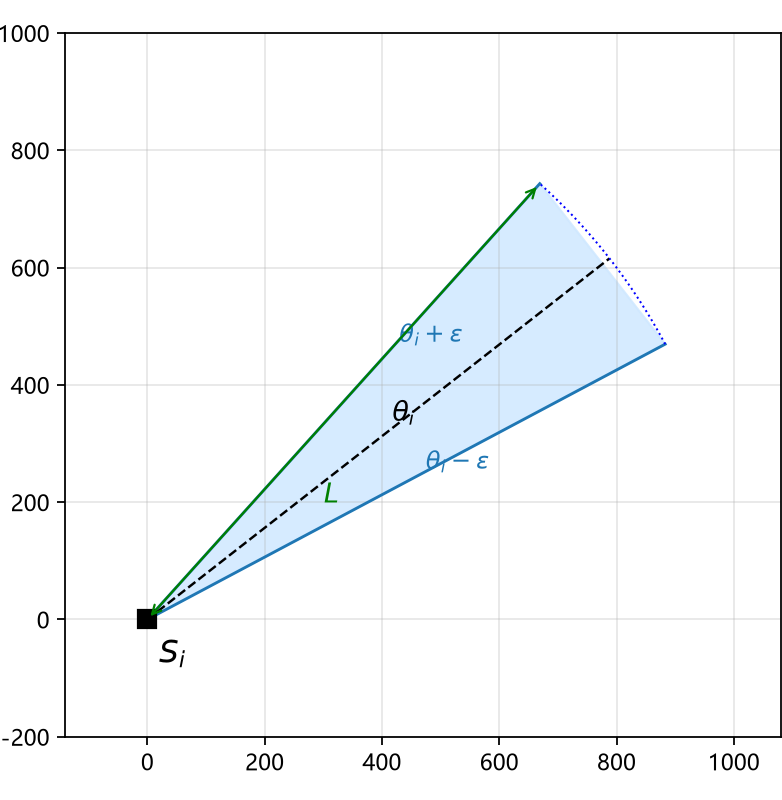
\includegraphics[width=0.46\textwidth]{figures/fig_p1_model_a.png}
		\caption{单检测点的楔形约束及其三角形近似}
		\label{fig:p1-wedge}
	\end{figure}
    
    \subsection*{4.1 \quad 模型建立}
    
	\subsubsection*{4.1.1 \quad 单检测点的楔形约束模型}
	在 \(S_i\) 处测得示向度 \(\theta_i\)，则真实方位角 \(\alpha_i\) 必落在
	\[
		\alpha_i\in[\theta_i-\varepsilon,\ \theta_i+\varepsilon].
	\]
	干扰源位于由 \(S_i\) 出发、方向为 \(\alpha_i\) 的射线上，射程未知。于是干扰源必落在以 \(S_i\) 为顶点、中心方向为 \(\theta_i\)、张角为 \(2\varepsilon\) 的楔形（角形扇形）内：
	\[
		W_i=\bigl\{\,S_i+t(\cos\alpha,\sin\alpha)\ :\ t\ge0,\ \alpha\in[\theta_i-\varepsilon,\ \theta_i+\varepsilon]\,\bigr\}.
	\]

	为便于作多边形运算，用三角形近似该楔形，其三个顶点为
	\[
		P_0=S_i,\quad
		P_1=S_i+L\bigl(\cos(\theta_i-\varepsilon),\sin(\theta_i-\varepsilon)\bigr),\quad
		P_2=S_i+L\bigl(\cos(\theta_i+\varepsilon),\sin(\theta_i+\varepsilon)\bigr).
	\]

	边长 \(L\) 的取法及其正确性. 目标域是半径 \(R\) 的圆域 \(\mathcal D_R\)，其中距 \(S_i\) 最远的点到 \(S_i\) 的距离为 \(\lVert S_i\rVert+R\)，这里 \(\lVert S_i\rVert=\sqrt{x_i^2+y_i^2}\)。只要取
	\[
		L=2\bigl(\lVert S_i\rVert+R\bigr)>\lVert S_i\rVert+R,
	\]
	则圆域内任意可能的干扰源位置都位于以 \(S_i\) 为心、半径 \(L\) 的圆内，从而必落在该三角形内。因此该三角形完全包含 \(W_i\cap\mathcal D_R\)，用它替代楔形只会多保留、绝不会漏掉任何可能位置，不改变最终交集。

	\subsubsection*{4.1.2 \quad 多检测点的定位区域模型}

\begin{figure}[H]
    \centering
    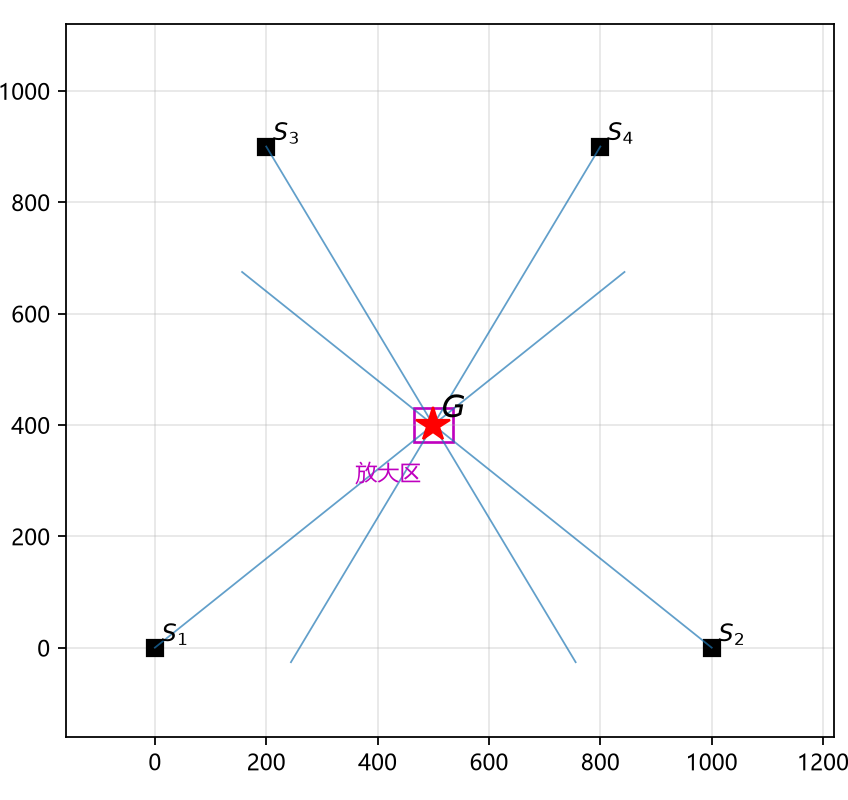
\includegraphics[width=0.7\textwidth]{figures/fig_p1_model_b.png}
    \caption{ 四个检测点的交会布局}
    \label{fig:p1-layout}
\end{figure}

干扰源必须同时满足所有检测点的约束。具体而言，在第 \(i\) 个检测点处，测得示向度 \(\theta_i\) 对应的角度约束为：
\[
\theta_i - \delta \le \text{atan2}(y-y_i, x-x_i) \le \theta_i + \delta,
\]
其中 \(\delta=1^{\circ}\)。该不等式在几何上定义了一个从检测点发出的楔形区域（三角形）\(W_i\)。

当存在 \(n\) 个检测点时，真实的干扰源必然落在所有 \(n\) 个楔形区域的交集内，同时受到目标圆域 \(\mathcal{D}_R\) 的限制。因此，最终的定位区域 \(\Omega\) 为各楔形交集与目标圆域之交：
\[
\Omega = \left(\bigcap_{i=1}^{n} W_i\right) \cap \mathcal{D}_R, \quad \mathcal{D}_R = \{(x,y) : x^2 + y^2 \leq R^2\}.
\]

关于该区域的几何性质：每个 \(W_i\)（三角形或扇形）与圆域 \(\mathcal{D}_R\) 都是凸集。根据凸集的性质，任意个凸集的交集必然仍为凸集，故定位区域 \(\Omega\) 是一个凸多边形。这一凸性具有极其重要的计算价值——它保证了后文在计算定位区域直径（即区域内任意两点间距离的最大值）时，最优解必定出现在多边形 \(\Omega\) 的某个顶点处，而无需考虑区域内部的奇异点，从而大幅降低了计算复杂度。

\subsubsection*{4.1.3 \quad 目标圆域的离散化及误差评估}


圆域不是多边形，为统一作多边形运算，用其内接正 64 边形近似。该多边形顶点精确落在半径 \(R\) 的圆上，每条边与真圆之间的最大偏差（矢高）为\[\Delta = R\Bigl(1-\cos\frac{\pi}{64}\Bigr) \approx 1800 \times (1-\cos 2.8125^{\circ}) \approx 2.17\,\text{m}.
\]
该偏差只在定位区域被圆域边界截断时才会影响结果。当 \(\Omega\) 完全落在圆域内部、圆域约束不起作用时，离散化不改变 \(\Omega\)。下文算例中 \(\Omega\) 位于 \((500, 400)\) 附近（到原点约 \(640\) m），远在半径 \(1800\) m 之内，故离散化的 \(2.17\) m 偏差对本例的直径与覆盖判定没有任何影响。作为一般原则，若要更保守，也可改用外接正多边形。

	

	\subsubsection*{4.1.4 \quad 定位区域直径的定义与计算依据}
	题目所说“定位区域直径”指点集直径，即区域内任意两点间距离的最大值：
	\[
		D=\max_{P,Q\in\Omega}\lVert P-Q\rVert .
	\]
	多边形直径必在顶点对取得. 固定 \(P\)，函数 \(Q\mapsto\lVert P-Q\rVert\) 是凸函数，它在凸多边形 \(\Omega\) 上的最大值必在某个顶点处取得；再固定该顶点 \(Q\)，同理最大值也在某个顶点 \(P\) 处取得。因此只需在所有顶点对中寻找最大距离：
	\[
		D=\max_{1\le j<k\le m}\lVert v_j-v_k\rVert,\qquad
		V=\{v_1,\dots,v_m\}\ \text{为}\ \Omega\ \text{的顶点集}.
	\]
	顶点数 \(m\) 通常很小（见 \S4.1），直接枚举顶点对（\(O(m^2)\)）即可。

	\subsubsection*{4.1.5 \quad “以多边形直径为直径的圆能否覆盖定位区域”的判据}
	设使直径 \(D\) 达到最大的顶点对为 \(P^*,Q^*\)，即 \(\lVert P^*-Q^*\rVert=D\)。以线段 \(P^*Q^*\) 为直径作圆，圆心 \(O=\tfrac12(P^*+Q^*)\)、半径 \(D/2\)，记为 \(\Gamma\)。

	这个圆是唯一可能的“以多边形直径为直径的圆”. 设某一以直径 \(D\) 为直径的圆（半径 \(D/2\)）能覆盖 \(\Omega\)，则它必包含相距 \(D\) 的两点 \(P^*,Q^*\)。而圆内任意两点的距离不超过其直径 \(D\)，等号当且仅当这两点恰是一对直径端点。故 \(P^*,Q^*\) 必是该圆的直径端点，圆心必为其中点 \(O\)。因此“以定位区域直径为直径的圆”被唯一确定为 \(\Gamma\)，是否覆盖 \(\Omega\) 不存在歧义。

	判据. 因 \(\Omega\) 是凸多边形、\(\Gamma\) 是圆盘（凸集），\(\Omega\subseteq\Gamma\) 当且仅当 \(\Omega\) 的所有顶点都落在 \(\Gamma\) 内：
	\[
		r^*:=\max_{1\le k\le m}\lVert v_k-O\rVert\le\frac{D}{2}
		\ \Longleftrightarrow\ \Gamma\ \text{覆盖}\ \Omega .
	\]
	又直径两端点 \(P^*,Q^*\) 到 \(O\) 的距离恰为 \(D/2\)，故恒有 \(r^*\ge D/2\)；于是覆盖成立当且仅当 \(r^*=D/2\)，即除直径两端点外，其余部分也不越出 \(\Gamma\)。

	\subsection*{4.2 \quad 算法设计}

	\subsubsection*{4.2.1 \quad 算法流程}

	\begin{enumerate}
		\item 初始化 \(\Omega\leftarrow\) 目标圆域的内接正 64 边形。
		\item 对每个检测点 \(S_i\)：按 \\S4.1.1 构造楔形三角形，令 \(\Omega\leftarrow\Omega\cap W_i\)；若 \(\Omega\) 变为空集则提前终止。
		\item 提取 \(\Omega\) 的全部顶点 \(V=\{v_1,\dots,v_m\}\)。
		\item 枚举顶点对求直径：\(D\leftarrow\max_{j<k}\lVert v_j-v_k\rVert\)，同时记录达到直径的顶点对 \(P^*,Q^*\)。
		\item 取圆心 \(O=\tfrac12(P^*+Q^*)\)、半径 \(D/2\)。
		\item 计算 \(r^*\leftarrow\max_k\lVert v_k-O\rVert\)，判定 \(\mathrm{covered}\leftarrow(r^*\le D/2+\text{容差})\)。
		\item 返回 \(D,\ O,\ r^*,\ \mathrm{covered}\)。
	\end{enumerate}

	\subsubsection*{4.2.2 \quad 核心几何运算的数学原理}

	（1）楔形三角形的构造. 直接由 \\S4.1.1 的顶点公式给出，取 \(L=2(\lVert S_i\rVert+R)\)。

	（2）凸多边形求交（半平面裁剪）. 两凸多边形之交仍是凸多边形，可依次用其中一个多边形的每条有向边所在直线去“裁剪”另一个多边形。设裁剪直线为 \(ax+by+c=0\)，定义线性符号函数 \(f(x,y)=ax+by+c\)，保留 \(f\ge0\)（或 \(f\le0\)）的一侧：沿多边形边界逐边行进，保留位于保留侧内的顶点，并在跨越裁剪线的边上按其与直线的比例插入交点，即得裁剪后的多边形。逐条边处理，最终结果就是两多边形的交集。整个过程只含加、乘、比较与线性插值，结果精确且始终保持凸性。

	（3）直径的计算. 由 \\S4.1.4，直接对所有顶点对计算欧氏距离并取最大；对凸多边形亦可用旋转卡壳法按 \(O(m)\) 完成。

	（4）覆盖圆的判定. 由 \\S4.1.5，圆心取直径线段中点、半径取 \(D/2\)，只需比较各顶点到圆心的距离与 \(D/2\)，无需求解一般的最小覆盖圆。

	\subsubsection*{4.2.3 \quad 计算复杂度}

	设当前多边形顶点数为 \(m\)。一次半平面裁剪为 \(O(m)\)，\(n\) 个检测点的总裁剪量为 \(O(nm)\)；直径枚举为 \(O(m^2)\)（采用旋转卡壳时为 \(O(m)\)）。由于 \(m\) 随有效约束边数增长，一般 \(m\le2n+64\)，故当 \(n\le10\) 时计算量极小，完全满足实时性要求。

	\subsection*{4.3 \quad 结果展示}

	\subsubsection*{4.3.1 \quad 仿真算例}

	题目未给出具体检测点与示向度，故构造一个可复现算例：设干扰源真值 \(G=(500,400)\) m，检测点
	\[
		S_1=(0,0),\quad S_2=(1000,0),\quad S_3=(200,900),\quad S_4=(800,900)\ (\text{m}),
	\]
	由几何关系反推各点示向度 \(\theta_i=\operatorname{atan2}(G_y-y_i,\ G_x-x_i)\bmod360^\circ\)，结果见表~\ref{tab:p1-bearing}。

	这里由真值反推的示向度是“理想读数”，但模型的不确定带为 \(\pm\varepsilon\)，故据此构造的每个楔形仍张 \(2^\circ\)，其交集仍是一个有面积的多边形。换言之，\(\varepsilon\) 表征的是读数本身固有的不确定度，而非多次读数之间的离散度，因此即使读数无误差，定位区域也不会退化为一个点。

	\begin{table}[H]
		\centering
		\caption{仿真算例的检测点与示向度}
		\label{tab:p1-bearing}
		\\begin{tabular}{ccc}
			\toprule
			检测点 & 坐标 (m) & 示向度 \(\theta_i\) (\(^\circ\)) \\
			\midrule
			\(S_1\) & (0, 0) & 38.66 \\
			\(S_2\) & (1000, 0) & 141.34 \\
			\(S_3\) & (200, 900) & 300.96 \\
			\(S_4\) & (800, 900) & 239.04 \\
			\bottomrule
		\end{tabular}
	\end{table}

	\subsubsection*{4.3.2 四个检测点的计算结果}

	对四个检测点求交，定位区域为 8 边形，结果见表~\ref{tab:p1-four}。

	\begin{table}[H]
		\centering
		\caption{四检测点算例的定位区域及其覆盖判定}
		\label{tab:p1-four}
		\begin{tabular}{cc}
			\toprule
			指标 & 数值 \\
			\midrule
			定位区域顶点数 \(m\) & 8 \\
			定位区域直径 \(D\) & 28.632 m \\
			直径端点 & \((500.000,414.516)\)、\((500.000,385.884)\) \\
			直径圆圆心 \(O\) & 约 \((500.000,400.203)\) \\
			半径 \(D/2\) & 14.316 m \\
			最远顶点距圆心 \(r^*\) & 14.316 m \\
			是否被直径为 \(D\) 的圆覆盖 & 是（\(r^*=D/2\)，相切） \\
			\bottomrule
		\end{tabular}
	\end{table}

	\subsubsection*{4.3.3 多检测点对比}

	保持同一干扰源真值 \(G=(500,400)\)，逐个追加上述检测点，各档结果见表~\ref{tab:p1-compare}。

	\begin{table}[H]
		\centering
		\caption{检测点数递增时的定位区域与覆盖性}
		\label{tab:p1-compare}
		\begin{tabular}{cccccc}
			\toprule
			检测点数 & 顶点数 \(m\) & 直径 \(D\) (m) & \(D/2\) (m) & \(r^*\) (m) & 覆盖（\(r^*\le D/2\)） \\
			\midrule
			2 & 4 & 35.772 & 17.886 & 17.886 & 是（相切） \\
			3 & 6 & 28.632 & 14.316 & 14.466 & 否（超出 0.150 m） \\
			4 & 8 & 28.632 & 14.316 & 14.316 & 是（相切） \\
			\bottomrule
		\end{tabular}
	\end{table}

	图~\ref{fig:p1-region}直观显示了三种情形的定位区域、直径线段、直径圆以及个别顶点越出圆外的情况。

	\begin{figure}[H]
		\centering
		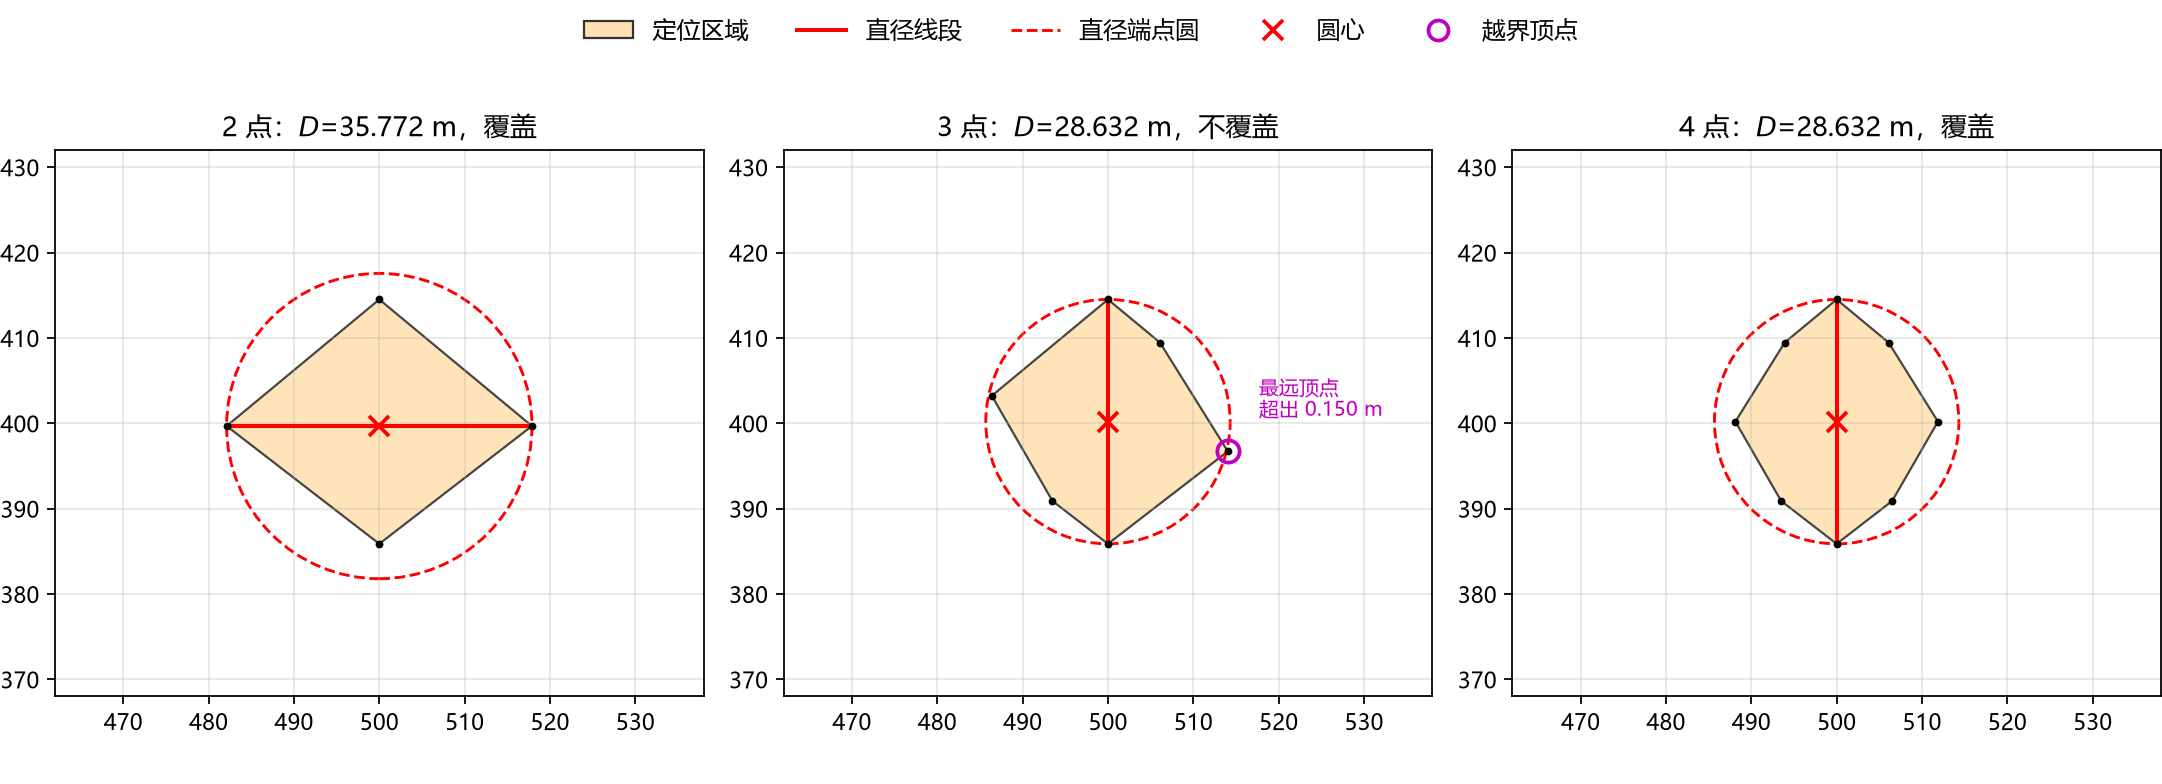
\includegraphics[width=0.96\textwidth]{figures/fig_p1_region.png}
		\caption{检测点个数不同时对应的定位区域、直径线段及其端点圆与覆盖判定}
		\label{fig:p1-region}
	\end{figure}

	\subsection*{4.4 结果分析}

	\subsubsection*{4.4.1 定位区域的性质}
	（1）顶点数的上界. 每个检测点贡献两条边界射线，\(n\) 个检测点最多产生 \(2n\) 条有效边界线；再计入圆域边界的贡献，顶点数 \(m\le2n+64\)。例如 \(n=3\) 时本例 \(m=6\)，\(n=4\) 时 \(m=8\)。

	（2）有界性. 由于始终与目标圆域求交，\(\Omega\) 恒有界。若仅用检测点约束，单个楔形区域的直径会趋向无穷（例如仅一个检测点、又无圆域约束时），此时“定位”无从谈起。

	\subsubsection*{4.4.2 直径与定位精度的关系}

	直径 \(D\) 是衡量定位精度的核心指标：\(D\) 越小，区域越紧凑，干扰源位置越确定。

	需要纠正一种想当然的说法：增加检测点只会使区域单调不增，而不是严格递减。因为新增一个约束只会取交集、使区域变小或不变，故直径不会增大；但若新检测点未改变当前区域的“最长跨度”，直径可保持不变。本例中 3 点与 4 点的直径完全相同（均为 \(28.632\) m）：第 4 个点只是削去了 3 点区域中越出直径圆的那个尖角（见 4.3 节），并未缩短最大跨度。此外，检测点的几何分布也显著影响 \(D\)：分散布置比聚集布置能更快缩小区域。

	\subsubsection*{4.4.3 覆盖性判定的结论}

	对一般凸多边形，直径圆通常不能覆盖定位区域；能否覆盖取决于区域的形状是否恰好“贴合”以直径线段为直径的圆。

	本例给出了三种典型情形（见表~\ref{tab:p1-compare}）：
	\begin{itemize}
		\item 2 点：覆盖（相切）。此时区域为四边形，其两条对角线分别长 \(35.772\) m 与 \(28.632\) m，直径取较长的水平对角线；另一对顶点距圆心仅约 \(14\) m，落在半径 \(17.886\) m 内，故被覆盖。
		\item 3 点：不覆盖。第 3 个楔形切去了四边形的一个斜角，却在 \((514.041,396.721)\) 处产生一个新顶点，它到圆心的距离为 \(14.466\) m，越出直径圆 \(0.150\) m，故不覆盖。
		\item 4 点：覆盖（相切）。第 4 个楔形恰把上述越界顶点削去，八个顶点全部落在圆内或圆上，故重新被覆盖。
	\end{itemize}

	作为对照，若允许圆心自由移动，定位区域的最小覆盖圆半径 \(r_{\min}\) 分别为 \(17.886\)m、\(14.317\)m、\(14.316\) m。由 Jung 定理，对平面点集恒有
	\[
		\frac{D}{2}\le r_{\min}\le\frac{D}{\sqrt3},
	\]
	但 \(r_{\min}\le D/2\) 不能作为“以多边形直径为直径的圆覆盖区域”的判据，因为固定圆心（直径线段中点）后所需的半径 \(r^*\) 一般会大于 \(r_{\min}\)。事实上，由于直径两端点相距 \(D\)，任何半径 \(D/2\) 的圆若同时含这两点，其圆心必为其中点，故 \\S4.1.5 的判据 \(r^*\le D/2\) 才是唯一正确的判据。

	\subsubsection*{4.4.4 误差传播分析}

	示向度误差 \(\varepsilon=1^\circ\) 对定位区域直径的影响可作如下估计：
	\begin{itemize}
		\item 当检测点与干扰源距离为 \(d\) 时，单条射线的横向误差约为 \(d\tan\varepsilon\approx0.0175\,d\)；
		\item 两条射线交会区域的特征尺寸与 \(d\) 成正比、与交会角 \(\phi\) 的正弦成反比：
		\[
			D\propto\frac{d\,\varepsilon}{\sin\phi};
		\]
		\item 因此，检测点应尽量分散，并与干扰源构成较大交会角，以缩小定位区域直径。此结论与问题二中由信息矩阵严格导出的“最优交会角 \(90^\circ\)”相互印证。
	\end{itemize}

	\subsubsection*{4.4.5 算法复杂度与实用性}

	\begin{table}[H]
		\centering
		\begin{tabular}{cc}
			\toprule
			操作 & 复杂度 \\
			\midrule
			单个楔形构造 & \(O(1)\) \\
			单个多边形裁剪 & \(O(m)\)，\(m\) 为当前顶点数 \\
			总求交（截断前） & \(O(nm)\) \\
			直径计算 & \(O(m^2)\)（旋转卡壳 \(O(m)\)） \\
			覆盖判定 & \(O(m)\) \\
			\bottomrule
		\end{tabular}
	\end{table}

	由于 \(m\le2n+64\)，实际 \(m\) 很小，算法在 \(n\le10\) 时计算量极小，完全满足实时性要求。

	\medskip
	\noindent 小结与衔接. 本问给出了“由示向度求定位区域、算其直径 \(D\)、并判断直径圆能否覆盖”的完整几何算法，其中 \(D\) 定量刻画了定位精度。问题二正是以此 \(D\) 为几何指标：在只有一个检测点时 \(D\) 无法确定（区域沿射线方向无界，直径趋于无穷），故必须合理选取第二检测点以最小化 \(D\)。



\section*{五、 问题二模型建立及求解}

	\subsection*{5.1 模型建立}
		问题二要求在已知 \(S_1\) 处示向度 \(\theta_1\) 的条件下确定第二检测点 \(S_2\) 及其候选区域，求解基于三点：单点不可定位——一个示向度只确定一条射线，源距 \(d_1\) 不可观测，必须引入第二检测点；误差逐点位固定——同一地点重复检测不改变误差，只有更换地点才呈现统计规律，故 \(S_2\) 必须是独立的新地点，且两地点误差可视为相互独立；源的位置与距离均未知——仅知真实方位角落在 \(\theta_1\pm\varepsilon\)（\(\varepsilon=1^\circ\)）、\(d_1\in(5,1500]\)，故源不确定集是二维的，策略须对其内任一点稳健。又有效接收半径在 \(1000\sim1500\) m 间未知，凡要求“第二次必定测到”处，须按半径下界 \(1000\) m 设计。

		沿用问题一的记号。两条带误差方向线交出四边形定位区域 \(\Omega\)，取其直径 \(D=\max_{P,Q\in\Omega}\lVert P-Q\rVert\) 为定位精度的几何度量（可由问题一算法直接计算）。信息层面用 Fisher 信息矩阵 \(F\) 刻画可辨识性，采用 D-最优准则 \(\max\det F\) 与 Frobenius 准则 \(\min\lVert F-\bar\lambda I\rVert^2\)（为 Zhao 等\cite{zhao2012} 所采用）。最终，源位置与距离均未知时以最坏情形直径为判据：
		\begin{equation}
			S_2^\ast=\arg\min_{S_2\in\mathcal F}\ \max_{G\in C}\ D(S_2;\,G),
			\label{eq:minimax}
		\end{equation}
		其中 \(C=\{d_1(\cos\delta_1,\sin\delta_1):d_1\in(5,1500],\,|\delta_1|\le\varepsilon\}\) 为源不确定集，\(\mathcal F\) 为保证探测的可行域（\S5.1.3）。

		\subsubsection*{5.1.1 坐标归一化与观测模型}
		平移并旋转坐标系，使 \(S_1\) 为原点、\(\theta_1\) 指向 \(x\) 轴正向。记源的真实角向偏差为 \(\delta_1\)（\(|\delta_1|\le\varepsilon\)），则 \(G=d_1(\cos\delta_1,\sin\delta_1)\)。设 \(S_2=(A,B)\)，对给定 \(G\) 记 \(d_2=\lVert G-S_2\rVert\)，交会角 \(\phi=\angle S_1GS_2\) 满足
		\begin{equation}
			\cos\phi=\frac{(S_1-G)\cdot(S_2-G)}{d_1d_2},\qquad \sin\phi=\sqrt{1-\cos^2\phi}.
			\label{eq:phi}
		\end{equation}
		单站单位方向向量观测模型为 \(\hat m_i=m_i+w_i\)（\(m_i=(S_i-G)/d_i\)，\(w_i\sim N(0,\sigma_i^2I)\)），相应 FIM 与两点叠加为
		
		\begin{equation}
			F_i=c_i^2\bigl(I-m_im_i^{\mathsf T}\bigr),\qquad
			F=F_1+F_2=\Bigl(\sum_{i=1}^{2}c_i^2\Bigr)I-\underbrace{\sum_{i=1}^{2}c_i^2\,m_im_i^{\mathsf T}}_{\mathcal G},\qquad c_i=\frac{1}{\sigma_i d_i}.
			\label{eq:F2}
		\end{equation}
		
		其中 \(\mathcal G=\sum_{i=1}^2 c_i^2m_im_i^{\mathsf T}\) 是由两个单位视线向量张成的加权投影和（框架算子）；因 \(\sum_i c_i^2\) 为常数，\(F\) 与 \(\mathcal G\) 只相差一个单位阵倍数，故 \(F\) 的几何信息全部含于 \(\mathcal G\)。
		
		单个检测点时 \(F_1\) 秩 \(1\)、\(\det F_1=0\)，\(d_1\) 不可辨识（Zhao 等命题 1 在 \(N=1\) 的退化情形），故第二检测点必要。由 \(m_1,m_2\) 夹角为 \(\phi\) 展开得
		
		\begin{equation}
			\det F=c_1^2c_2^2\sin^2\phi,\qquad
			\lVert F\rVert^2=\bigl(c_1^2+c_2^2\bigr)^2-2c_1^2c_2^2\sin^2\phi,
			\label{eq:det}
		\end{equation}
		
		两者均只通过 \(\sin^2\phi\) 依赖几何，在 \(\phi=90^\circ\) 同时最优（二维下两准则等价）。令 \(\varphi_i=c_im_i\)，则 \(\mathcal G=\sum_i\varphi_i\varphi_i^{\mathsf T}\)；框架理论\cite{zhao2012} 给出两点最优当且仅当 \(\{\varphi_i\}\) 为紧框架，即 \(\sum_i c_i^2m_im_i^{\mathsf T}=\tfrac12(c_1^2+c_2^2)I\)。无论 \(d_1=d_2\)（正则）或 \(d_1\neq d_2\)（非正则，不规则度 \(k_0=1\)），均推出 \(m_1\perp m_2\)。故当源距离已知时，两点最优交会角恒为 \(90^\circ\)，与距离比无关。

		需说明 FIM 的适用性：题设误差逐点位固定、有界，本不宜套用随机误差的 CRLB；但附录2称“不同地点才呈现统计规律”，故把各点固定偏差视为对称分布的一次抽样（跨地点零均值、异地独立），FIM 即“跨地点平均”意义下的可辨识性，适合用于选点。且 \(\sigma_1=\sigma_2\) 时 \(c_i\propto1/d_i\)，最优几何只依赖距离比而与分布形状无关。因此用 FIM 确定最优几何与可观测性，而把保证型精度指标交给有界误差下的直径 \(D\)。

		\subsubsection*{5.1.2 交会定位区域直径}
		两条 \(\pm\varepsilon\) 边界线在交会点附近各近似为一对平行线（间距 \(2d_1\sin\varepsilon\)、\(2d_2\sin\varepsilon\)），其交叠区域为平行四边形，邻边长为 \(2d_i\sin\varepsilon/\sin\phi\)、夹角 \(\phi\)，取较长对角线得
		\begin{equation}
			D=\frac{2\sin\varepsilon}{\sin\phi}\sqrt{d_1^2+d_2^2+2d_1d_2|\cos\phi|}.
			\label{eq:D}
		\end{equation}
		\(D\) 在 \(\phi=90^\circ\) 最小，最小值为 \(2\sin\varepsilon\sqrt{d_1^2+d_2^2}\)（\(d_1=d_2\) 时为 \(2\sqrt2\,d\sin\varepsilon\)），即源距离已知时 FIM 最优几何同时使直径最小。

		\subsubsection*{5.1.3 保证探测约束}
		取保证半径 \(R=1000\) m（接收半径下界），要求 \(\max_{G\in C}\lVert G-S_2\rVert\le R\)。距离函数对 \(G\) 是凸的，最大值必在 \(C\) 的极点取得；\(C\) 的极点为 \(d_1\in\{5,1500\}\) 与 \(\delta_1\in\{-\varepsilon,\varepsilon\}\) 的组合，故约束等价于四个圆盘
		\begin{equation}
			(A-x_k)^2+(B-y_k)^2\le R^2,\quad k=1,\dots,4,
			\label{eq:lens}
		\end{equation}
		其中 \((x_k,y_k)=(d\cos\delta,d\sin\delta)\)，\(d\in\{5,1500\}\)、\(\delta\in\{-\varepsilon,\varepsilon\}\)。满足其的点集是透镜形可行域 \(\mathcal F\)。此处必用半径下界：只有按最小可能半径设计，才能保证真实半径偏小时第二次测向仍成功。

	\subsection*{5.2 模型求解}
		\subsubsection*{5.2.1 已知 \(d_1\) 的最优布站}
		\(\phi=90^\circ\) 等价于 \(G\) 在以 \(S_1S_2\) 为直径的圆上；若 \(d_1\) 已知，取 \(d_2=d_1\) 得等腰直角三角形，
		\begin{equation}
			S_2=S_1+d_1\sqrt2\,\bigl(\cos(\theta_1\pm45^\circ),\ \sin(\theta_1\pm45^\circ)\bigr).
			\label{eq:known}
		\end{equation}

		\subsubsection*{5.2.2 未知源位置：两条稳健准则}
		准则甲（保证交会角）：求 \(\max_{S_2\in\mathcal F}\min_{G\in C}\sin\phi\)。\(\delta_1=0\) 时 \(\sin\phi=|B|/d_2\) 的最小值在距 \(A\) 较远端点取得；令 \(S_2\) 取可行域顶点并使两端点等距，得解析解
		\begin{equation}
			A^\ast=\frac{5+1500}{2}=752.5\ \text{m},\qquad
			B^\ast=\sqrt{R^2-\Bigl(\frac{1500-5}{2}\Bigr)^2}=664.3\ \text{m},
			\label{eq:criterionA}
		\end{equation}
		即 \(\psi^\ast=41.4^\circ\)、\(\min\phi=41.6^\circ\)。计入二维不确定集（\(\delta_1=\pm1^\circ\)）后最优点略移至 \(S_2=(764.0,651.0)\) m、\(\psi=40.4^\circ\)，保证 \(\min_{G\in C}\phi=39.6^\circ\)，最坏 \(D=134.8\) m。

		准则乙（最小最坏直径）：直接对 \eqref{eq:D} 在 \(\mathcal F\) 内全局寻优，得
		\begin{equation}
			S_2=(801.0,\ 605.0)\ \text{m},\quad L=1003.8\ \text{m},\quad \psi=37.1^\circ,
			\label{eq:criterionB}
		\end{equation}
		最坏源为 \(d_1=1500\) m、\(\delta_1=+1^\circ\)，此时 \(\max_{G\in C}D=134.1\) m、\(\min_{G\in C}\phi=36.2^\circ\)。两准则最优点均在可行域外缘（\(L\approx1004\) m），偏转角不同：准则甲换取更大的角度保证，准则乙换取更小的直径。结果汇总于表~\ref{tab:p2-plan}。

		\begin{table}[H]
			\centering
			\caption{两种稳健准则的最优布站与最坏指标（\(R=1000\) m，\(\varepsilon=1^\circ\)，\(C\) 内取最坏）}
			\label{tab:p2-plan}
			\begin{tabular}{lccccc}
				\toprule
				准则 & \(A\)/m & \(B\)/m & 偏转角 \(\psi\) & \(\min_{G\in C}\phi\) & 最坏 \(D\)/m \\
				\midrule
				甲：保证交会角 & 764.0 & 651.0 & \(40.4^\circ\) & \(39.6^\circ\) & 134.8 \\
				乙：最小最坏直径 & 801.0 & 605.0 & \(37.1^\circ\) & \(36.2^\circ\) & 134.1 \\
				（无约束理想值）\(\phi=90^\circ\) & --- & --- & \(90^\circ\) & \(90^\circ\) & 49.4 \\
				\bottomrule
			\end{tabular}
		\end{table}
		表中“无约束理想值”指 \(d_1=d_2=R=1000\)、\(\phi=90^\circ\) 时的直径，它不满足 \eqref{eq:lens}，仅作精度参照；因保证半径被迫取 \(1000\) m，真正可达的最坏直径约 \(134.1\sim134.8\) m。

		\subsubsection*{5.2.3 算法流程}
		整个求解是确定性的（无随机数），输入为 \(S_1,\theta_1\) 及本题常量 \(\varepsilon=1^\circ\)、\(R=1000\) m。首先确定第二检测点的偏转角：按准则乙取 \(\psi\approx37^\circ\)，若侧重交会角保证则按准则甲取 \(\psi\approx40^\circ\)；据此在 \(S_2=S_1+L(\cos(\theta_1\pm\psi),\sin(\theta_1\pm\psi))\) 处布下第二点，其中 \(L\approx1004\) m，两支互为镜像、任选一支。到达 \(S_2\) 后测得新的示向度 \(\theta_2\)，用问题一算法求出定位区域 \(\Omega\) 及其直径 \(D\)。最后以 \(D\) 为精度判据形成闭环：若 \(D\le20\) m 即可光学精定位并清除；若 \(D>20\) m，则沿 \(\Omega\) 中心方向递进重测，直至进入 \(20\) m 范围。

	\subsection*{5.3 结果及分析}
		模型验证。 用精确四线交点对 \eqref{eq:D} 随机验证：\(45^\circ\le\phi\le135^\circ\) 内 \(292\) 组样本的平均相对偏差 \(6.4\times10^{-4}\)、最大 \(1.9\times10^{-3}\)，说明 \eqref{eq:D} 在有效交会区内足够精确。

		最优布站几何（图~\ref{fig:p2-geometry}）。 图~\ref{fig:p2-geometry}(a) 显示，当 \(d_1\) 已知时两射线在源处成 \(90^\circ\)，源落在以 \(S_1S_2\) 为直径的圆上；取等腰直角使 \(d_2=d_1\)，即得式 \eqref{eq:known} 的构造。图~\ref{fig:p2-geometry}(b) 中三个点划线圆盘之交即保证探测的透镜形可行域 \(\mathcal F\)，两准则最优点（三角、圆圈）均落在该透镜外缘，说明基线已被“必然可测”约束顶满、不宜再短。

		\begin{figure}[H]
			\centering
			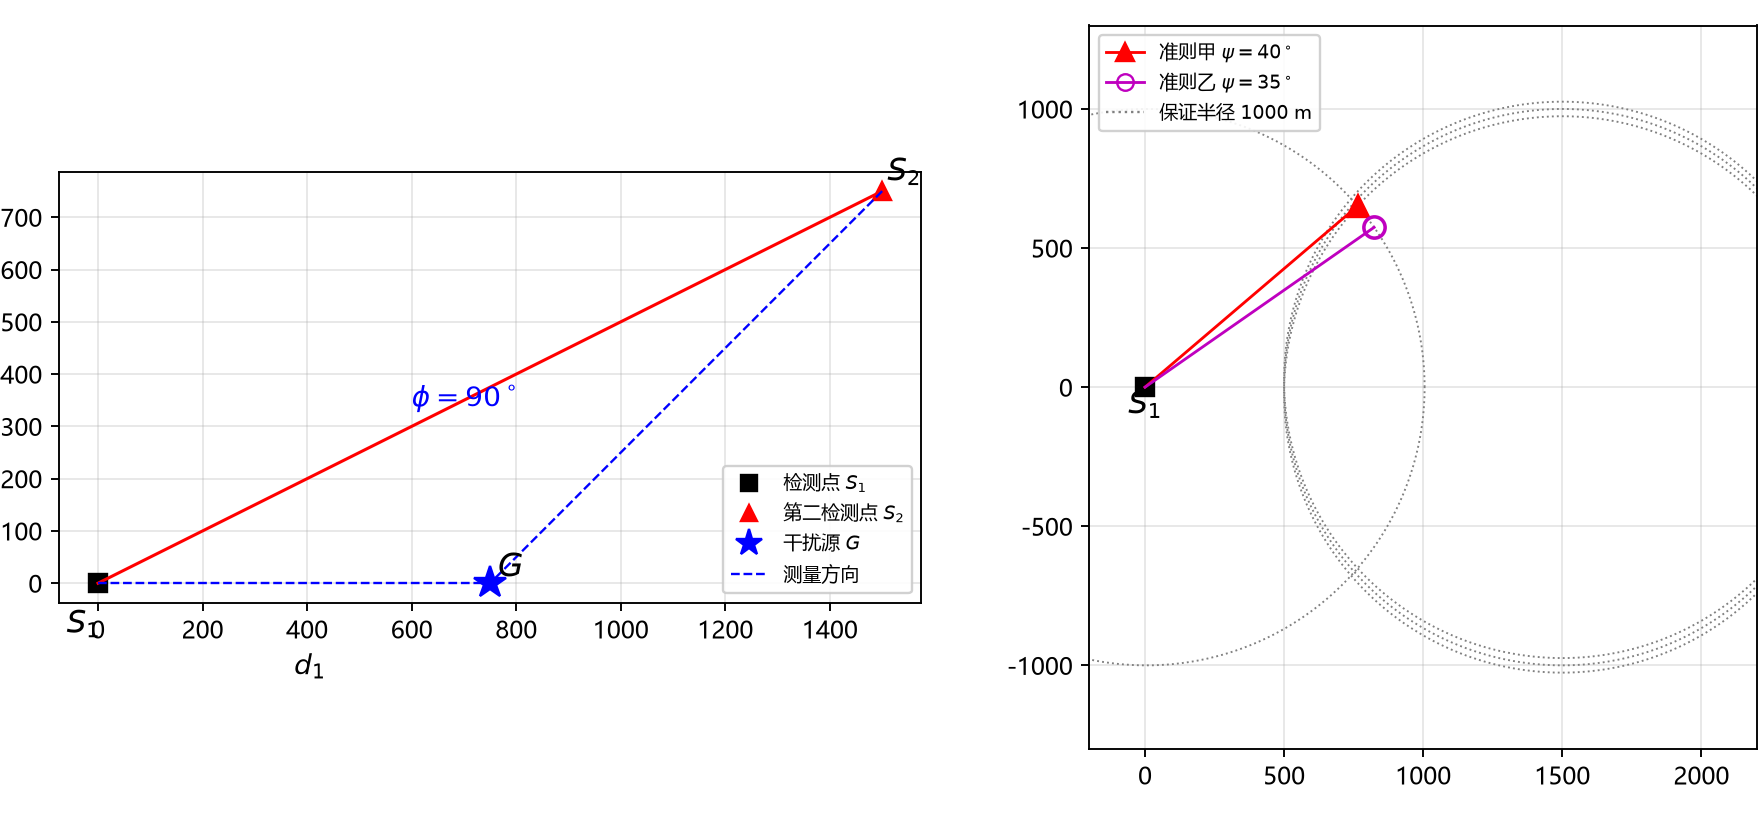
\includegraphics[width=0.88\textwidth]{figures/问题二最优布站几何.png}
			\caption{(a) 已知 \(d_1\) 的等腰直角构造（\(\phi=90^\circ\)）；(b) \(d_1\) 未知时两条稳健推荐方向。}
			\label{fig:p2-geometry}
		\end{figure}

		交会角与最坏直径（图~\ref{fig:p2-dphi}、\ref{fig:p2-heat}）。 图~\ref{fig:p2-dphi} 的每条曲线为 \eqref{eq:D} 在给定 \((d_1,d_2)\) 下随 \(\phi\) 的变化，皆以 \(1/\sin\phi\) 为主导：\(\phi\) 减小则 \(D\) 单调增大，在 \(\phi=90^\circ\) 取最小（星号），\(\phi\to0^\circ\) 时发散——这正是必须避开近似共线构型、追求大交会角的原因。图~\ref{fig:p2-heat} 的颜色为对源不确定集 \(C\) 取最坏的 \(\max_{G\in C}D\)：低值（深色）谷底沿透镜外缘呈弧形，两个标记（红星为准则甲、红圈为准则乙）正落在这一低值带内；透镜之外为不可行区。

		\begin{figure}[H]
			\centering
			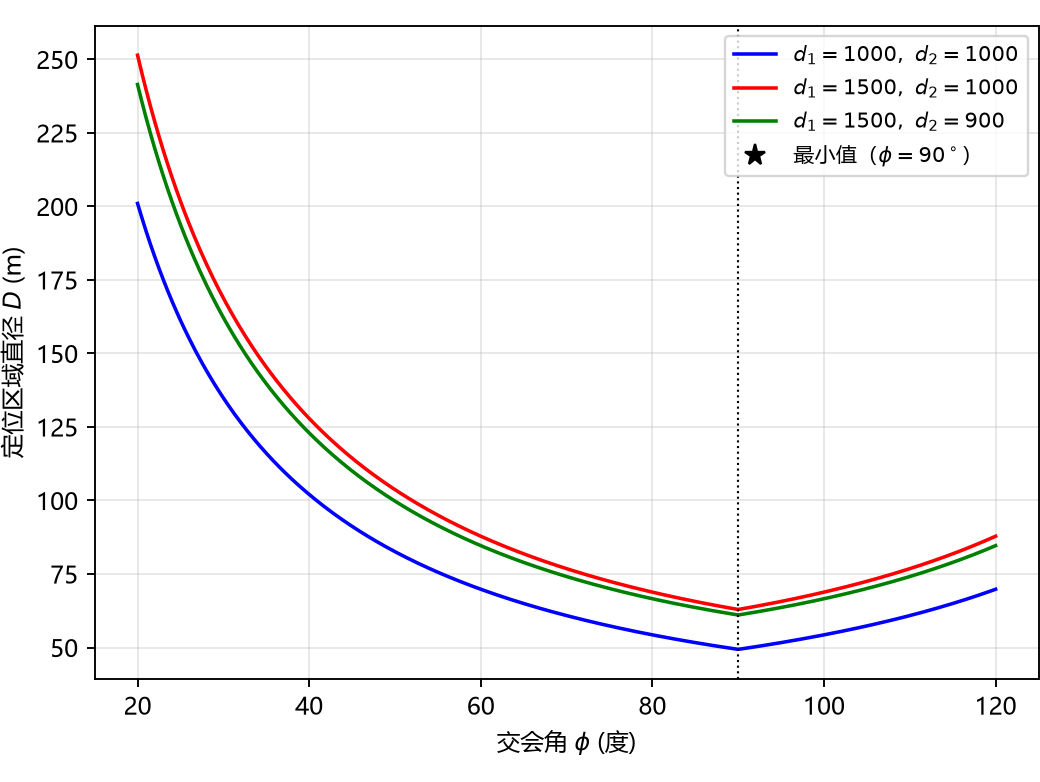
\includegraphics[width=0.62\textwidth]{figures/位区直径随交会角的变化.png}
			\caption{定位区直径 \(D\) 随交会角 \(\phi\) 的变化}
			\label{fig:p2-dphi}
		\end{figure}

		\begin{figure}[H]
			\centering
			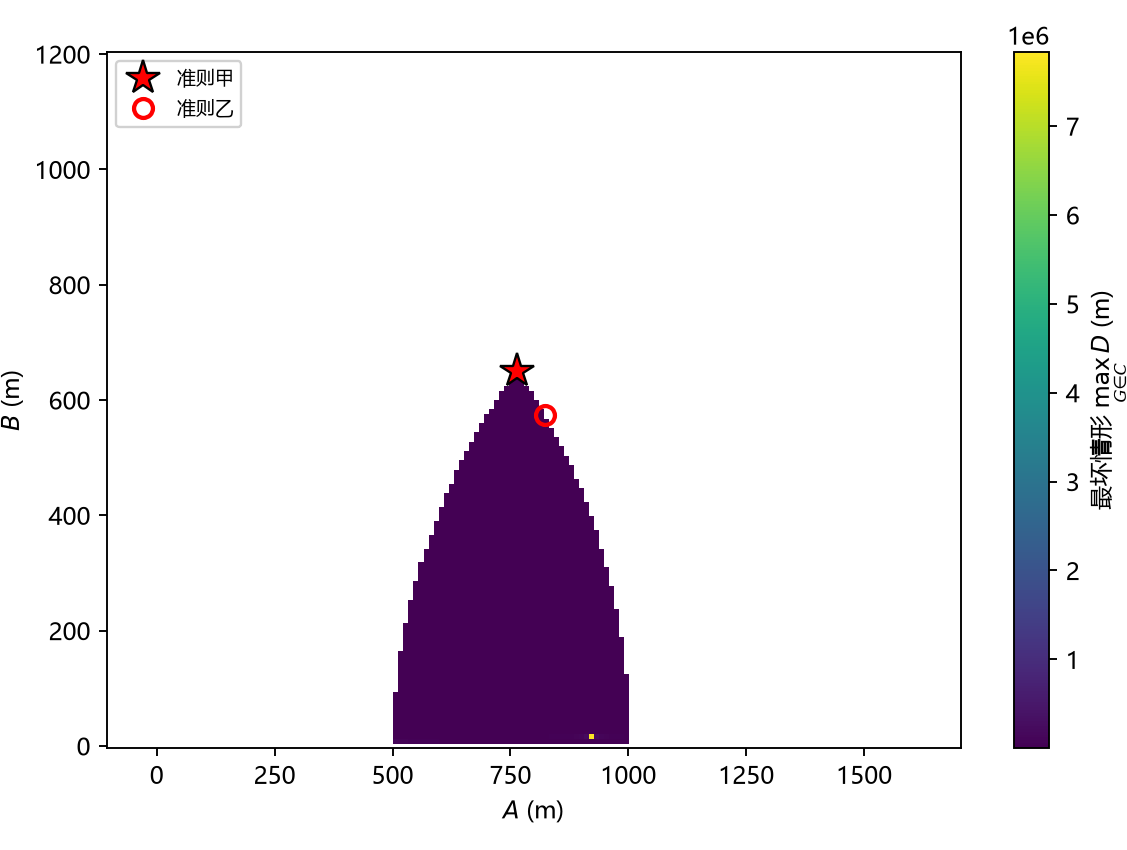
\includegraphics[width=0.62\textwidth]{figures/稳健点推荐.png}
			\caption{未知源时第二点的最坏定位直径分布}
			\label{fig:p2-heat}
		\end{figure}

		候选区域。 因最终判据是最坏直径，候选区域由“最坏直径不超过最优值 \(1+\eta\) 倍”直接定义（\(\eta=10\%\)）：
		\begin{equation}
			\mathcal C=\Bigl\{S_2\in\mathcal F:\ \max_{G\in C}D(S_2;G)\le(1+\eta)D^\ast\Bigr\},\qquad D^\ast=134.1\ \text{m},
			\label{eq:candidate}
		\end{equation}
		该口径与目标函数 \eqref{eq:minimax} 一致，由定义必含两准则最优点。数值上 \(\mathcal C\) 满足 \(A\in[726,910]\) m、\(B\in[401,646]\) m，即 \(S_1\) 为极点时径向距离 \(r\in[948,1004]\) m、方位角 \(\theta_1\pm[25^\circ,40^\circ]\)，单瓣面积约 \(0.010\ \text{km}^2\)（两瓣合计 \(0.021\ \text{km}^2\)）。推荐落点为 \(\psi\approx37^\circ\)（准则乙）或 \(\psi\approx40^\circ\)（准则甲）、距 \(S_1\) 约 \(1004\) m 处的两条对称方向，两瓣等价，可按现场路径任选。

		\begin{figure}[H]
			\centering
			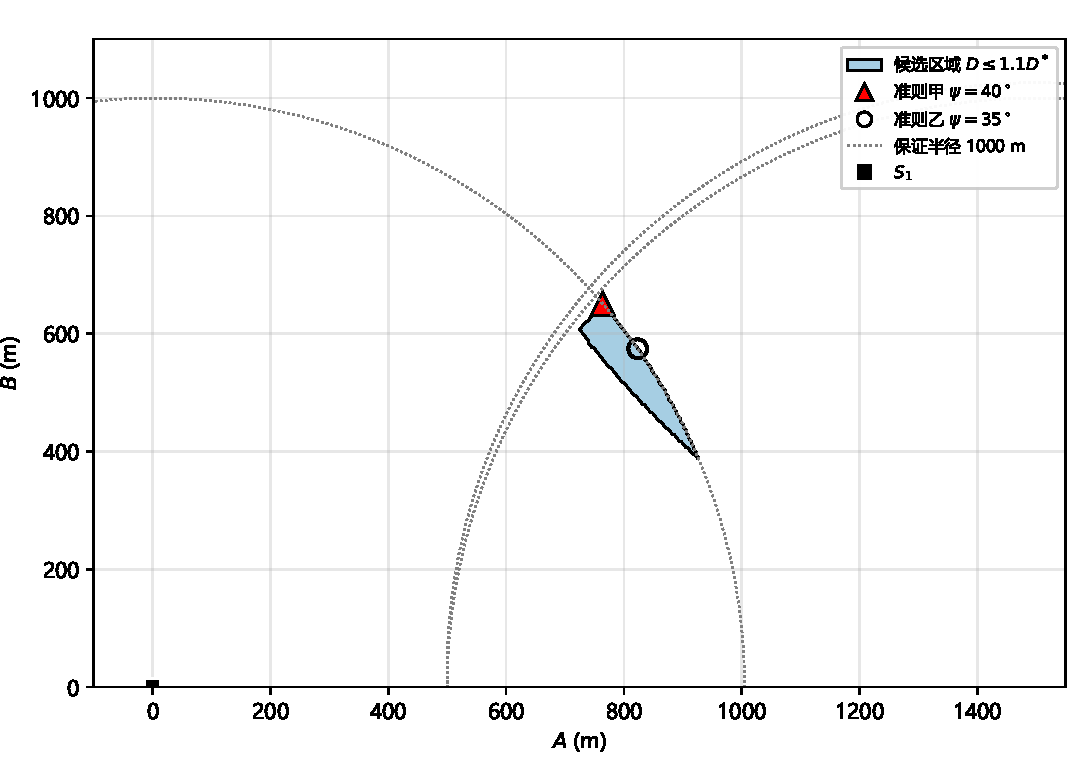
\includegraphics[width=0.62\linewidth]{figures/T2候选区.pdf}
			\caption{第二检测点候选区域与两条准则的推荐落点。}
			\label{fig:p2-region}
		\end{figure}

		灵敏度分析。 （1）对测向误差：由 \eqref{eq:D} 有 \(D\propto\sin\varepsilon\)，近似线性，提高测向精度比增大基线更直接有效。（2）对源距离：\(D(d_1)\) 呈先减后增的 U 形，最坏值在 \(d_1=1500\) m 处取得（图~\ref{fig:p2-sens-b}），这正是必须对 \(d_1\) 取最坏的原因。（3）对保证半径：\(R\) 由 \(1000\) m 放宽到 \(1500\) m（乐观口径）时最坏直径由约 \(123\) m 降到约 \(104\) m（图~\ref{fig:p2-sens-c}）；本文取保守口径以硬保证第二次测向成功，若允许失败后补测则可采用乐观口径。（4）对误差系统性：FIM 的 CRLB 偏乐观，故以可直接计算的有界误差直径 \(D\) 为主指标；两准则最坏 \(D\) 均超 \(120\) m，远大于 \(20\) m 阈值，故第二阶段必须采用“递进靠近 + 光学精定位”闭环，不能一次交会即定。

		\begin{figure}[H]
			\centering
			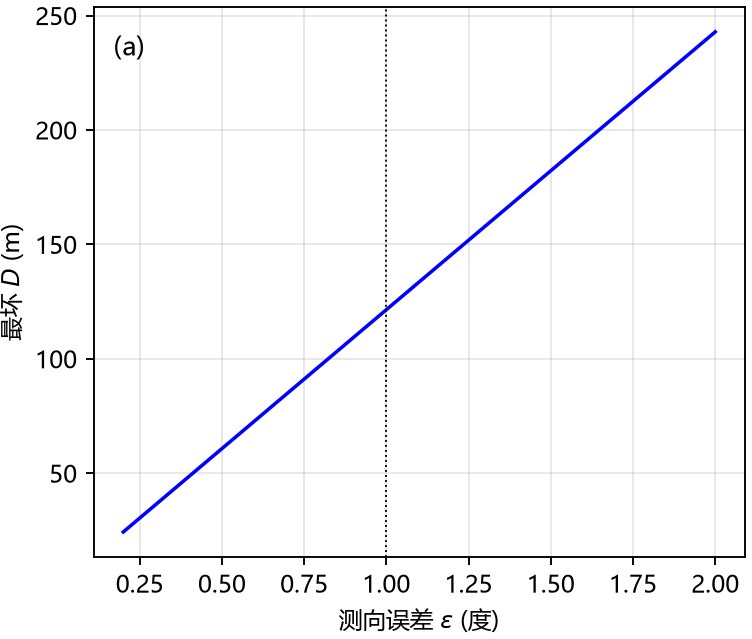
\includegraphics[width=0.62\textwidth]{figures/灵敏度分析_a.png}
			\caption{\(D\) 对 \(\varepsilon\) 的变化}
			\label{fig:p2-sens}
		\end{figure}

		\begin{figure}[H]
			\centering
			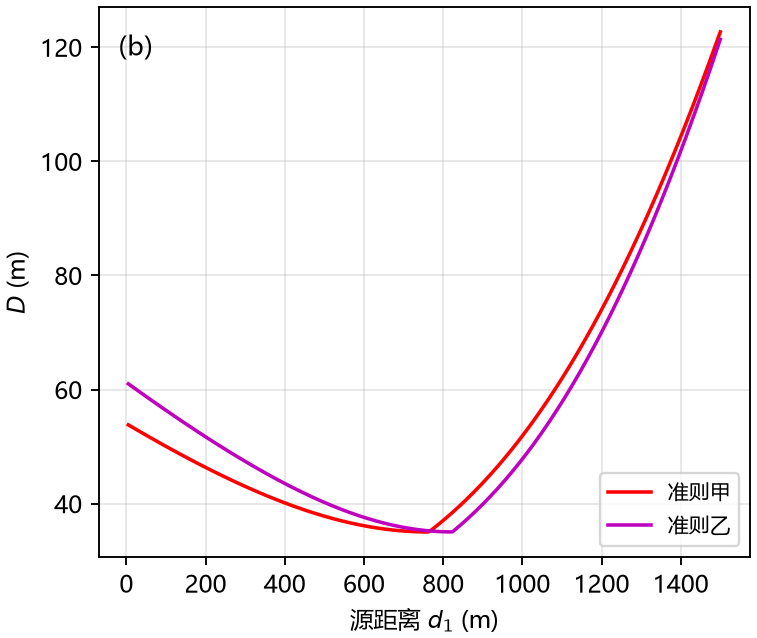
\includegraphics[width=0.62\textwidth]{figures/灵敏度分析_b.png}
			\caption{\(D\) 随 \(d_1\) 的变化}
			\label{fig:p2-sens-b}
		\end{figure}

		\begin{figure}[H]
			\centering
			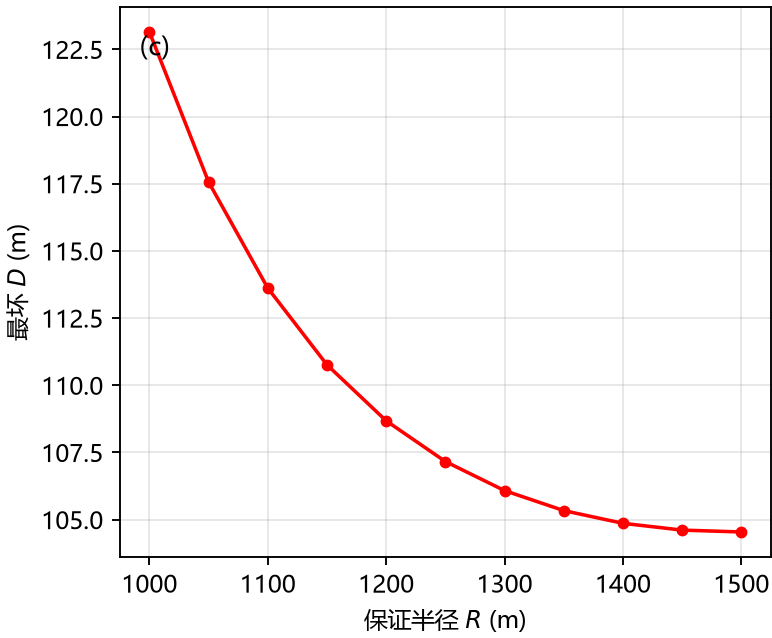
\includegraphics[width=0.62\textwidth]{figures/灵敏度分析_c.png}
			\caption{最坏 \(D\) 对保证半径 \(R\) 的变化}
			\label{fig:p2-sens-c}
		\end{figure}

\section*{六、  问题三模型建立及求解}
	\subsection*{6.1 模型建立}
	该目标区域中的干扰源均为全向干扰源，总共有 10-16 个，但具体个数未知。现机器狗从原点出发，测向机初始频道为 1，对目标区域干扰源进行自动定位并清除。要求在确保所有干扰源被清除的前提下，完成任务的时间越短越好。需要我们制定机器狗自动搜索定位及清除的策略，并设计相应的算法。对全向干扰源而言，测向机能否检测到信号只取决于检测点与干扰源之间的距离。设某干扰源为 \(G\)，其有效接收半径为$R_G \in [1000,1500]$.若机器狗在检测点 \(S\) 处满足$|SG| \le R_G$,则测向机可以接收到该干扰源信号，并测得示向度。

    由于 \(R_G\) 未知，但一定不小于 \(1000\) 米，因此可以采取保守策略：只要检测点 \(S\) 满足$|SG| \le 1000$,
    则无论该干扰源的实际有效接收半径是多少，都一定能检测到它。也就是说，若机器狗在某个检测点，以该点为圆心、半径 \(1000\) 米的圆覆盖了干扰源位置，则该干扰源必然可被检测。
    
    反过来，因为干扰源位置未知，要保证目标区域中任意位置的干扰源都能被检测到，就需要选择若干检测点，使得以这些检测点为圆心、半径 \(1000\) 米的圆能够覆盖整个目标区域。于是问题转化为：
    
    \begin{quote}
    用多少个半径为 \(1000\) m的圆，才能完全覆盖半径为 \(1800\) m的目标圆域？
    \end{quote}
    根据全等圆盘覆盖问题（disk covering problem）的经典结果：用 7 个全等圆盘完全覆盖单位圆盘时，所需最小半径比为 $\rho_7=\boldsymbol{\dfrac12}$；用 6 个圆盘时该最小半径比为 $\rho_6\approx \boldsymbol{0.5559052}$（Bezdek 1979 的证明，OEIS A299695；5 个对应 Bezdek 1983，$\rho_5\approx 0.6093829$，OEIS A133077）。本题中小圆与大圆半径之比为 $\dfrac{5}{9}\approx 0.5555556$，恰满足
\[
0.5=\rho_7<\dfrac{5}{9}<\rho_6\approx 0.5559052.
\]
由此可知，7 个半径为 1000\,m 的小圆可以实现对目标大圆的全覆盖，而仅使用 6 个小圆则无法完成覆盖（即便 6 圆摆到该族最优，也需覆盖半径 $1000.6294$\,m，比可用的 1000\,m 只差 $0.629$\,m，短差比仅 $0.063\%$）。

本文程序实际采用的 7 点布局为均匀布局：7 个覆盖圆的圆心都落在以原点为圆心、半径 $1000$\,m 的圆上，且均匀分布（正七边形顶点，每 $360^\circ/7\approx 51.43^\circ$ 一个），相邻圆心间距 $867.77$\,m。覆盖校验：圆域内任一点到最近圆心 $\le 1000$\,m，最坏点恰在原点（距离 $=1000.0000$\,m，零余量）。该布局仍严格成立——因为覆盖判据是“圆心到源距离 $\le 1000$\,m $\le$ 源有效接收半径下界”，原点处恰好取等而非越界；其单重覆盖比例 $28.5\%$、平均覆盖重数 1.96。从原点出发走完 7 个圆心的最短开放路径为 $6206.60$\,m。

\begin{figure}[H]
    \centering
    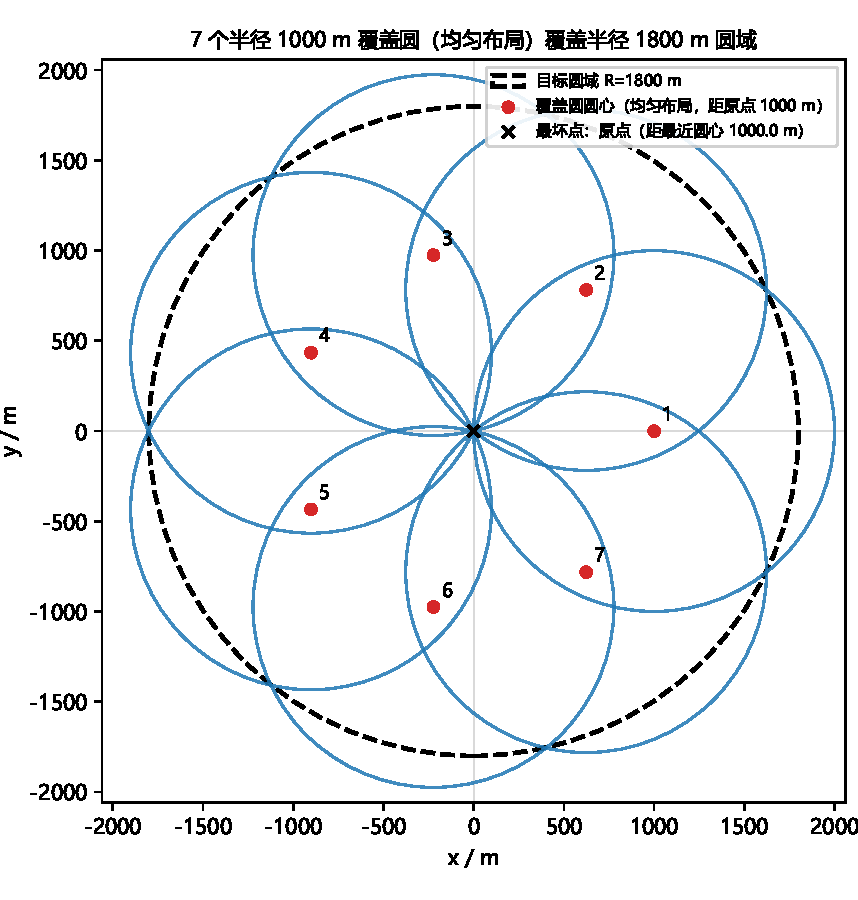
\includegraphics[width=0.45\textwidth]{figures/7_circles.pdf}
    \caption{均匀布局：7 个半径为 1000\,m 的覆盖圆覆盖半径 1800\,m 的目标圆域}
    \\label{fig:t3-circles}
\end{figure}

\begin{table}[H]
    \centering
    \caption{ 覆盖圆方案与巡视路线关键参数（均匀布局，程序缺省）}
    \label{tab:t3-cover}
    \begin{tabular}{lcc}
        \toprule
        参数 & 取值 & 单位 \\
        \midrule
        最少覆盖圆数 \(k\) & 7 & 个 \\
        布局最坏最近距离（恰在原点） & 1000.0000 & m \\
        巡视里程（原点起最短开放路径） & 6206.60 & m \\
        纯移动时间（\(v=5\)\,m/s） & 1241.32 & s \\
        \bottomrule
    \end{tabular}
\end{table}

	\subsection*{6.2 指标定义}

为量化评估确定性两阶段搜索与清除策略的性能，定义以下指标：

\begin{itemize}
    \item 虚拟总时长：机器狗移动、测向、切换频道及清除操作消耗的虚拟时钟总和，单位为秒（s）。
    \item 平均定位清除时长：单局平均定位清除每个干扰源所耗的虚拟时长，单位为秒(s)。
    \item 清除比例：成功清除的干扰源数量与总干扰源数量的比值。
    \item 定位误差：估计位置与实际位置之间的欧氏距离，用于衡量多视角交会定位的精度。
    \item 顺路清除命中：顺路清除成功次数与无效往返次数的比值，用于评估“顺路清除”策略在巡视过程中的有效性。
\end{itemize}

\subsection*{6.3 搜索与清除模型}

\subsubsection*{6.3.1覆盖与巡视路径模型}
目标区域为半径 \(R=1800\text{m}\) 的圆域。采取 7 站覆盖圆布局，保证区域内任意点到最近观测站的距离不超过有效接收半径下界 \(\rho_{\text{min}}=1000\text{m}\)。巡视顺序被建模为从原点出发遍历 7 个观测站的最短开放路径问题，用 Held--Karp 动态规划精确求解（状态数 \(O(2^7\cdot7^2)\)，非 \(7!\) 枚举），得巡视里程 \(L_{\text{survey}}=6206.60\text{m}\)，顺序 \(2\to1\to0\to6\to5\to4\to3\)。旋转自由度模型保证：均匀布局的 7 个站等距原点（均为 1000\,m），将布局绕原点整体旋转，既不改变覆盖保证（只依赖点间距离与点到原点距离），也不改变该开放路径长度（首段与各段均只依赖点间距离），因此旋转是零成本自由度，可用于对准源密集方向。

\subsubsection*{6.3.2起点全频道扫描与布局定向模型}
机器狗在原点 \((0,0)\) 对全部 20 个频道各测向一次，一次性获取“哪些频道在接收范围内、从原点看它们各在哪个方向”。设听到的示向度集合为 \(\mathcal{B} = \{b_1,\dots,b_m\}\)。定义最密集方向 \(\theta^*\) 为：
\begin{equation}
\theta^* = \arg \max_{\phi \in [0^{\circ},360^{\circ})} \left| \{ b \in \mathcal{B} : \Delta_\theta(b, \phi) \leq 30^{\circ} \} \right|
\end{equation}
其中 \(\Delta_\theta(\cdot,\cdot)\) 为两方位角在 \([0^\circ,180^\circ]\) 内的最小夹角。窗口宽 \(60^\circ\)，逐 \(1^\circ\) 扫描全圆，并在“装入个数不减少”的前提下用窗口内示向度的圆均值做亚度精修。取目标方位 \(\theta_{\text{first}} = \theta^* - 90^{\circ}\)，若第一站原方位为 \(\phi_0\)，则布局整体旋转 \(\Delta\phi = \theta_{\text{first}} - \phi_0 \pmod{360^{\circ}}\)，使第一点正对最密集方向顺时针 \(90^{\circ}\) 的方位。设计意图：使阶段一先扫外围开阔方向，把源密簇留给后续站位与阶段二。

\subsubsection*{6.3.3 定位区域与两条物理前提}

由问题一，每次测得示向度 \(\theta\) 给出一个楔形约束 \(W_i\)，多次测量的可能源集合为各楔形之交与目标圆域之交：
\begin{equation}
    \Omega=\Bigl(\bigcap_{i} W_i\Bigr)\cap \mathcal{D}_R,\qquad
    \mathcal{D}_R=\{(x,y):x^2+y^2\le R^2\},
\end{equation}
取 \(\Omega\) 的最小覆盖圆（MEC）圆心作为位置估计（构造与凸性见 \S4.1，问题三沿用同一口径）。整个策略建立在此区域之上，并由题面给出两条物理前提：

\begin{enumerate}
    \item 同一地点误差固定，同点复测无新增信息。题面指出测向误差是地点的属性，同一地点重复检测不改变误差，只有换到不同地点误差才呈现统计规律。因此信息必须来自新地点（实际应用中以相距 60m 以上为判断标准）。通常两条不同视角的射线已足以定出交会区域，实测每源平均采集 \(2.3\) 条示向度（\(131\) 个源中 \(91\) 个两条即收敛）。
    \item 测量结果都是硬约束。全向源收得到当且仅当 \(d\le R_{\text{rec}}\in[1000,1500]\text{m}\)，故一次测量可判出：收得到（\texttt{direction}）\(\Rightarrow\) 源在某测量点的 \(1500\text{m}\) 圆盘内；收不到（\texttt{no\_signal}）\(\Rightarrow\) 源在某测量点的 \(1000\text{m}\) 圆盘外。前者用外接多边形、后者用内接多边形近似，确保真源永不被切掉。\texttt{no\_signal} 尤其关键：它把“什么都没听到”变成实质的排除约束，将只含一条射线的贯穿长带压成有限的一段，并可在后续巡视中可证明地跳过该频道的测量。实测 seed 0--9 共跳过 \(160\) 次（每局 \(16\) 次），按每次 \(5\text{s}\) 测向 \(+1\text{s}\) 切换计约省 \(960\text{s}\)，占 10 局总时长约 \(2.7\%\)。
\end{enumerate}

\subsubsection*{6.3.4 两阶段清除模型}
整个清除流程按“先顺路、后专程”分两阶段推进。阶段一为巡视扫描：定义活跃频道集 \(\mathcal{A}\)，机器狗沿 7 站覆盖路径逐站扫描，采用“够准即停”裁剪，当定位区域最小覆盖圆半径 \(<20\text{m}\) 时不再测向，此时估计已落在清除半径内，再测只会徒增 \(6\text{s}\)。顺路清除只在巡视站到站后触发，由两个入口筛选待清频道：前向方位扇区（“本站\(\to\)圆心”与“下一站\(\to\)圆心”夹成的较短弧，估计点距原点限 \([d_{\min},d_{\max}]\)）与到站后近距（距当前站 \(\leq r_{\text{near}}\)）。起点段与后向清除逻辑已被移除，保证顺路清除始终基于当前最新定位信息做前向决策（详见 \S6.3.5）。该阶段不改变巡视顺序、不额外绕路，命中即是净收益，落空也只是一次 \(3\text{s}\) 试清的代价。

巡视结束后，仍未清除的频道转入阶段二（定位与清除）。以 \(\Omega\) 的最小覆盖圆圆心为估计点，按“就近试清 \(\to\) 多点覆盖试清 \(\to\) 文献准则补测 \(\to\) 末端逼近”四级递进，每一级的定位精度更高、动作代价也更大。第一级就近试清在最小覆盖圆半径 \(\le 400\text{m}\)（估计不离谱）时直接走到估计点 \texttt{/clear} 一次：清除半径仅 \(20\text{m}\)，走到源的近处本就是清除的必要动作，故到达后顺手一试的边际代价只有失败时的 \(3\text{s}\)，命中则省去整轮补测；实测阶段二所清源中 \(91.1\%\)（\(72/79\)）在这一级一次命中。未命中则进入第二级多点覆盖试清，用至多 \(K=7\) 个半径 \(20\text{m}\) 的圆贪心覆盖整个 \(\Omega\) 并依次试清，不寄望于单点估计，而是用 \(7\) 个 \(20\text{m}\) 圆对整个可能区域容错探清；实测 \(2/79\) 源由此命中。

若仍不行，第三级文献准则补测会新增一条示向度以收窄 \(\Omega\)。补测点按 Fisher 信息准则选取，位置的预测协方差为
\begin{equation}
    J=\sum_i \frac{1}{\sigma^2 r_i^{2}}\,n_i n_i^{\!\top},\qquad
    \sigma_{\text{pos}}=\sqrt{\operatorname{tr}(J^{-1})},
\end{equation}
其中 \(n_i\) 为第 \(i\) 条射线的单位法向量、\(r_i\) 为检测点到假设源的距离、\(\sigma=1^\circ\)。该式同时体现文献的两条结论——检测点越贴近源、新射线与已有射线交角越接近正交，预测 \(\sigma\) 越小。两条等距观测在夹角 \(\varphi\) 时 \(\sigma_{\text{pos}}\propto 1/|\sin\varphi|\)：取 \(r=1000\text{m}\)、\(\sigma=1^\circ\)，交会角由 \(30^\circ\) 增到 \(90^\circ\) 可使 \(\sigma_{\text{pos}}\) 由 \(49.4\text{m}\) 降到 \(24.7\text{m}\)。程序在每个假设源位置周围枚举 \(24\) 个方位角 \(\times\) \(5\) 档半径（\(150\sim800\text{m}\)）的候选点，先剔除与已有射线共线的退化点，再按对全部假设位置的平均 \(\sigma\) 升序、并列（相差 \(2\%\) 内）时取里程最短者排序。实测每局平均仅补测 \(0.5\) 次。

最后一级末端逼近兜底：沿最新实测示向度以 \(16\text{m}\) 步长逐步逼近（步数按到区域最远顶点距离自适应，\(24\sim120\) 步），以消除沿视线方向的定位偏差，保证“定位略偏也能清除”。四级递进的代价结构可由表~\ref{tab:t3-methods} 的清除方式分布印证：阶段一顺路与阶段二首次试清两级合计解决 \(52+72=124\) 个源，占 \(94.7\%\)，而需要多点覆盖与补测回升的仅 \(7\) 个（\(5.3\%\)），末端逼近在本批一次未触发。绝大多数源都在最便宜的前两级完成，只有定位困难者才逐级升级，这正是递进设计把总代价压在低端的原因。

\begin{table}[H]
    \centering
    \caption{ 清除方式分布（seed 0--9，共 131 个源）}
    \label{tab:t3-methods}
    \begin{tabular}{lcc}
        \toprule
        清除方式 & 次数 & 占比 \\
        \midrule
        阶段一·巡视顺路清除 & 52 & 39.7\% \\
        阶段二·就近试清一次命中 & 72 & 55.0\% \\
        阶段二·多点覆盖试清命中 & 2 & 1.5\% \\
        阶段二·补测后清除 & 5 & 3.8\% \\
        \midrule
        合计 & 131 & 100\% \\
        \bottomrule
    \end{tabular}
    \par\smallskip
    \footnotesize{注：阶段二四级流程中前三级的命中分布；末端逼近为兜底，本批未触发。}
\end{table}

\subsubsection*{6.3.5 基于方位扇区与覆盖圆约束的动态顺路清除模型}

在阶段一的巡视扫描过程中，基础模型采取“点对点”刚性巡视，即当前站任务完成后直接前往下一站。为降低冗余移动代价，本节建立动态顺路清除模型，将“专程往返”转化为“顺路清除”。

\paragraph{触发时机}
该模型仅发生在巡视站到站后（即完成本站扫描后）。起点段以及后向（上一站区间）的清除逻辑已被移除，确保所有顺路清除均基于当前最新的定位信息进行前向决策。

\paragraph{双入口筛选机制}
在每次巡视站到站后，通过以下两个入口筛选待清除的干扰源：

    前向顺路入口（方位扇区约束）：设干扰源估计点 \(E\)、当前巡视站 \(P_{\text{at}}\) 与下一巡视站 \(P_{\text{next}}\) 相对于圆心的方位角分别为 \(\theta_{\text{est}}\)、\(\theta_{\text{at}}\) 与 \(\theta_{\text{next}}\)。若估计点方位 \(\theta_{\text{est}}\) 落在 \(\theta_{\text{at}}\) 与 \(\theta_{\text{next}}\) 夹成的较短弧内，则判定该源为“顺路可清”。这一几何关系等价于角度空间上的三角不等式：
    \begin{equation}
    \Delta_\theta(\theta_{\text{est}}, \theta_{\text{at}}) + \Delta_\theta(\theta_{\text{est}}, \theta_{\text{next}}) \leq \Delta_\theta(\theta_{\text{at}}, \theta_{\text{next}}) + \epsilon
    \end{equation}
    其中，\(\Delta_\theta(\alpha, \beta)\) 定义为两个方位角 \(\alpha\) 与 \(\beta\) 在 \([0^\circ, 180^\circ]\) 区间内的最小夹角，\(\epsilon\) 为极小的数值容差（用于抵抗计算机浮点数运算的微小误差）。该式的几何本质是：当点 \(E\) 落在两站夹角内部时，其到两端点的角距离之和恰好等于两端点自身的角距离；若落在夹角外部，该和将严格大于两端点角距离，从而被判定为不顺路。
    
    特别地，此处必须使用真实的夹角 \(\Delta_\theta(\cdot, \cdot)\)，而绝不能使用正弦值（如 \(|\sin(\theta_1 - \theta_2)|\)）进行替代。因为在正弦函数中，相差 \(180^\circ\) 的反方向点（\(\sin 180^\circ = 0\)）会被误判为同向点，这会导致机器狗跑向完全错误的方向，产生严重的无效往返。
    
    此外，估计点到圆心的距离需限制在 \([d_{\min}, d_{\max}]\) 区间内（\(d_{\min}, d_{\max}\) 分别为前向顺路估计点距原点距离的下、上界）。筛选后，候选源按沿扇区方位的距离由近到远排序。
    近距顺路入口（近邻约束）：取消方位限制，直接筛选距离当前站 \(\leq r_{\text{near}}\)（\(r_{\text{near}}\) 为近距清除半径）的估计点，并按距离由近到远排序。


\paragraph{共同门槛：区域置信度约束}
无论从哪个入口进入，参与顺路清除的频道必须满足定位区域最小覆盖圆半径 \(\leq \rho_{\text{mec}}\)（\(\rho_{\text{mec}}\) 为区域半径上限）。若定位区域过大，顺路清除的命中概率极低，算法将其直接移交给阶段二补测收窄与兜底逼近机制处理。该门槛配合方位扇区与近距双入口，使无效往返被压缩到很低水平（同源 10 局演练合计白跑 13 次，约 1.3 次/局）。

\paragraph{清除动作：覆盖圆圆心法}
对满足门槛的频道，以定位区域的最小覆盖圆（MEC）为几何依据生成试清点：先取 MEC 圆心作为第一试清点，再用贪心覆盖选点判断 \(K=7\) 个半径 \(20\text{m}\) 的圆能否盖满整个定位区域——若能盖满，则把包括 MEC 圆心在内的全部圆心都纳入试清点（此时真源必落在某个圆内，逐个试清必定命中）；若盖不满（区域过大），则只保留 MEC 圆心一点，以免在低概率区域徒增无效往返。随后把试清点按距当前位置由近到远排序，依次进行光学精确定位与清除：一旦命中，该频道立即进入已清除状态，后续各站不再对其测向、也不再参与阶段二调度；若试清点全部落空，则将其移交阶段二补测收窄与兜底逼近。

\paragraph{模型优势与实证效果}
该模型将清除动作融入巡视移动，具有以下优势：
\begin{enumerate}
    \item 零额外规划成本：巡视路径长度仅依赖站点间距离，该模型不改变巡视顺序，路径规划成本为零。
    \item 高概率低成本试探：顺路清是“顺路碰运气”，只挑命中概率高的频道（区域小、盖满必中），只花便宜的成本（顺路移动 + 失败仅 3s），拿不下的（大区域、盖不满）毫不犹豫交给阶段二兜底。
    \item 实测显著收益：在 seed 0--9 的同源 10 局演练中，顺路清除合计命中 52 个、白跑 13 次（约 5.2 命中/局），无效往返被压到很低水平。10 局虚拟总时长均值 3613.6s、里程均值 14113.9m。上述参数经由优化确定（见 \S6.4 末“参数优化”），对宽区间内的时间变化不敏感，具有良好的鲁棒性。
\end{enumerate}

\subsection*{6.4模型求解}

模型采用确定性算法求解，全程无随机数，同种子下逐字节可复现。

求解依次按“先扫描、再定向、后路径与调度”展开。起点全频道扫描求解时，机器狗在原点连续测量 20 个频道，由于连续测向存在频道切换，耗时模型为 \(20 \times 5\text{s} + 19 \times 1\text{s} = 119\text{s}\)，此步骤获取初始示向度集合 \(\mathcal{B}\)，并标记无信号频道。随后进行密集方向求解，采用窗宽 \(60^{\circ}\)、步长 \(1^{\circ}\) 的滑动窗口遍历全圆，结合圆均值进行亚度精修，最终得到 \(\theta^*\) 和布局旋转角 \(\Delta\phi\)。巡视路径与阶段二遍历顺序求解采用 Held-Karp 算法精确求解最短开放路径，状态转移方程为
\begin{equation}
dp[S][i] = \min_{j \in S, j \neq i} \bigl( dp[S \setminus \{i\}][j] + d(j,i) \bigr)
\end{equation}
最终得出 \(n \leq 16\) 时毫秒级的精确解。最后是阶段二调度求解：四级流程由优先级队列进行状态调度，补测候选点按 Fisher 预测 \(\sigma\) 最小优先选方向（见 \S6.3.4），并强制与已有检测点保持 \(\geq 60\text{m}\) y以上间距。


\paragraph{参数优化}
上述顺路清除的四个参数（前向距离下界 \(d_{\min}\)、前向距离上界 \(d_{\max}\)、近距清除半径 \(r_{\text{near}}\)、区域半径上限 \(\rho_{\text{mec}}\)）并非凭经验给定，而是由优化算法自动确定。考虑到单局结果受场景随机性影响较大、直接以平均总时长最短为目标的搜索容易拟合种子噪声，本文改用更稳健的\textbf{组内方差}作为优化目标：以坐标下降（两轮）框架，对每个参数沿其可行区间做三分搜索，每次评价为固定 21 局（7 个干扰源个数 \(\times\) 3 个随机种子）演练的统计量；目标函数为“按干扰源个数分组、组内求方差再对各组取平均”，约束为平均总时长相对基准的涨幅不超过 \(1.5\%\) 且每局必须全部清除。搜索集（21 局）与独立采样的留出集（21 局）共同用于检验，最终收敛的最优值为 \(d_{\min}^*=296.3\)、\(d_{\max}^*=1296.3\)、\(r_{\text{near}}^*=377.8\)、\(\rho_{\text{mec}}^*=103\)（单位 m）。表~\ref{tab:t3-inline} 给出各参数的搜索区间与最优值，表~\ref{tab:t3-var} 给出优化前后的指标对照：方差指标在留出集上由 \(25831.9\) 降至 \(25413.9\ \text{s}^2\)，而平均总时长基本持平（\(3620.5\to3608.4\)\,s），说明该组参数在保证效率的同时具有更好的稳定性，且在较宽的参数区间内对时间变化不敏感。

\begin{table}[H]
    \centering
    \caption{顺路清除 4 参数的搜索区间与最优值}
    \label{tab:t3-inline}
    \begin{tabular}{llcc}
        \toprule
        符号 & 度量对象 & 搜索区间/m & 最优值/m \\
        \midrule
        \(d_{\min}\) & 估计点\(\to\)原点 & \([0,1000]\) & 296.3 \\
        \(d_{\max}\) & 估计点\(\to\)原点 & \([1000,1800]\) & 1296.3 \\
        \(r_{\text{near}}\) & 估计点\(\to\)巡视站 & \([0,600]\) & 377.8 \\
        \(\rho_{\text{mec}}\) & 定位区域 MEC & \([20,300]\) & 103.0 \\
        \bottomrule
    \end{tabular}
    \par\smallskip
    \footnotesize{注：MEC 为定位区域的最小覆盖圆；优化方法见上文“参数优化”。}
\end{table}

\begin{table}[H]
    \centering
    \caption{以组内方差为指标的参数优化效果}
    \label{tab:t3-var}
    \begin{tabular}{llccc}
        \toprule
        数据集 & 参数 & 平均总时长/s & 组内方差/s\(^2\) & 组内 \(\sigma\)/s \\
        \midrule
        \multirow{2}{*}{搜索集（21 局）} & 优化前基准 & 3662.8 & 50778.4 & 225.3 \\
                                        & 优化后取值 & 3671.9 & 32252.5 & 179.6 \\
        \multirow{2}{*}{留出集（21 局）} & 优化前基准 & 3620.5 & 25831.9 & 160.7 \\
                                        & 优化后取值 & 3608.4 & 25413.9 & 159.4 \\
        \bottomrule
    \end{tabular}
    \par\smallskip
    \footnotesize{注：组内方差按干扰源个数 \(n\) 分组、组内求方差后再对 \(n\) 取均值；优化约束为平均总时长涨幅 \(\le 1.5\%\) 且每局全清。}
\end{table}

\subsection*{6.5结果及分析}

\subsubsection*{6.5.1算法结果}
基于离线演练同源模拟器，按程序缺省均匀布局（\texttt{--layout uniform}）在 seed 0-9 的 10 局测试中（共 \(N=131\) 个干扰源），算法总体表现如表~\ref{tab:t3-overall}。该批数据可由 \texttt{python -m t3 --practice 10 --seed 0 --layout uniform} 逐字节复现。

\begin{table}[H]
    \centering
    \caption{ 总体成绩（seed 0--9，\(N=131\) 个干扰源）}
    \label{tab:t3-overall}
    \begin{tabular}{lcc}
        \toprule
        指标 & 数值 & 说明 \\
        \midrule
        清除比例 & \(131/131=100\%\) & 10 局全部清完，0 失败 \\
        平均定位清除时间 & 275.8\,s/个 & 总虚拟时长 \(\div\) 清除源数 \\
        虚拟总时长 & \(3613.6\pm294.8\)\,s & 范围 3212.5--4093.4\,s \\
        定位误差 & 均值 7.69\,m / 最差 17.94\,m & 全部 \(<20\)\,m 清除半径 \\
        顺路清除 & 命中 52 / 白跑 13 & 约 5.2 命中/局 \\
        \bottomrule
    \end{tabular}
\end{table}

表~\ref{tab:t3-overall} 给出策略在 10 局演练上的总体表现。清除比例 \(131/131=100\%\)、10 局 0 失败，说明“全清”这一硬约束在随机场景下稳定成立，策略的可靠性不依赖特定种子。虚拟总时长 \(3613.6\pm294.8\)\,s，极差 \(3212.5\)--\(4093.4\)\,s，相对标准差约 \(8.2\%\)；由于同一 seed 逐字节可复现，这一波动并非算法抖动，而是源空间布局随机性带来的固有余量，也提示单局时长不足以评价策略，须以多局长统计为准。定位误差均值 \(7.69\)\,m、最差 \(17.94\)\,m，全部落在 \(20\)\,m 清除半径内，但最差一例距半径仅余 \(2.06\)\,m，恰好解释了清除方式分布中仍有约 \(5\%\) 的源无法一次试清、需要多点覆盖或补测的原因。顺路清除命中 \(52\) 次、白跑 \(13\) 次，命中率约 \(80\%\)，无效往返每次仅耗 \(3\)\,s，代价在总时长中可忽略。

\begin{table}[H]
    \centering
    \caption{不同干扰源个数下的策略性能}
    \label{tab:t3-sweep}
    \begin{tabular}{cccccc}
        \toprule
        \multirow{2}{*}{干扰源个数 \(n\)} & \multirow{2}{*}{局数} &
            \multicolumn{2}{c}{总虚拟时长 / s} &
            \multicolumn{2}{c}{平均清除时间 / (s/个)} \\
        \cmidrule(lr){3-4}\cmidrule(lr){5-6}
            & & 均值 & 标准差 & 均值 & 标准差 \\
        \midrule
        10 & 10 & 3425.7 & 346.4 & 342.6 & 34.6 \\
        11 & 10 & 3657.3 & 219.5 & 332.5 & 20.0 \\
        12 & 10 & 3535.1 & 208.2 & 294.6 & 17.3 \\
        13 & 10 & 3751.3 & 328.1 & 288.6 & 25.2 \\
        14 & 10 & 3860.8 & 220.7 & 275.8 & 15.8 \\
        15 & 10 & 3852.2 & 241.6 & 256.8 & 16.1 \\
        16 & 10 & 3808.0 & 293.4 & 238.0 & 18.4 \\
        \midrule
        合计 & 70 & 3698.6 & 299.7 & 284.5 & --- \\
        \bottomrule
    \end{tabular}
    \par\smallskip
    \footnotesize{注：每个 \(n\) 使用固定 seed 集（\(\text{seed}=2026+1000n+k\)，\(k=1,\dots,10\)），同 seed 逐字节可复现；“合计”行的平均清除时间为总虚拟时长 \(\div\) 总源数 \(910\)。}
\end{table}

表~\ref{tab:t3-sweep} 显示：随 \(n\) 增大，总虚拟时长在 3.4--3.9\,ks 区间内缓慢上升并趋于饱和，而平均每个源的清除时间由 \(342.6\) 近单调降至 \(238.0\)\,s/个——源越多，巡视阶段一次扫描可同时服务更多源，规模效应明显；70 局总时长标准差约 \(300\)\,s，波动主要来自源空间布局的随机性。全过程动作分解虚拟总时长（seed 0--9 均值 \(3613.6\)\,s）见表~\ref{tab:t3-break}。

\begin{table}[H]
    \centering
    \caption{虚拟总时长构成（seed 0--9，均值 \(3613.6\)\,s）}
    \label{tab:t3-break}
    \begin{tabular}{lcc}
        \toprule
        构成项 & 时长 / s & 占比 \\
        \midrule
        移动（里程 14113.9\,m，\(v=5\)\,m/s） & 2822.8 & 78.1\% \\
        测向（120.3 次 \(\times\) 5\,s） & 601.5 & 16.6\% \\
        频道切换 + 清除 + 规划 & 189.3 & 5.2\% \\
        \midrule
        合计 & 3613.6 & 100\% \\
        \bottomrule
    \end{tabular}
\end{table}

移动路径已双最优（巡视 Held--Karp、阶段二精确最短开放路径），逼近下界；测向已被“够准即停”“无信号禁区跳过”“升序省切换”充分裁剪，故两大部分合计约占 95\%，进一步压缩空间有限。

三次正式模拟的全局形态见图~\ref{fig:three}、图~\ref{fig:three-b}、图~\ref{fig:three-c}。图中最外实线圆为半径 \(1800\,\text{m}\) 的作业圆域，内侧虚线圆为半径 \(1770\,\text{m}\) 的干扰源生成域；7 个细线圆是覆盖圆，各圆心按巡视访问顺序编号。机器狗自原点出发，先在原地完成一次全频道扫描取得初始示向度，再沿最短开放路径依次巡视 7 个圆心。测向点、无信号点与清除成功点大多落在巡视干线及其邻域，说明清除动作已被嵌入巡视过程，只有少数频道需偏离干线专程处理，正对应阶段一顺路清除与阶段二定位清除的分工。图中未见长距离往返折返，从过程形态上印证了表~\ref{tab:t3-break} 中移动耗时约占 \(78.1\%\)、巡视路径已取最短开放路径的判断，直观支撑“先顺路、后专程”的分阶段设计。

\begin{figure}[H]
  \centering
  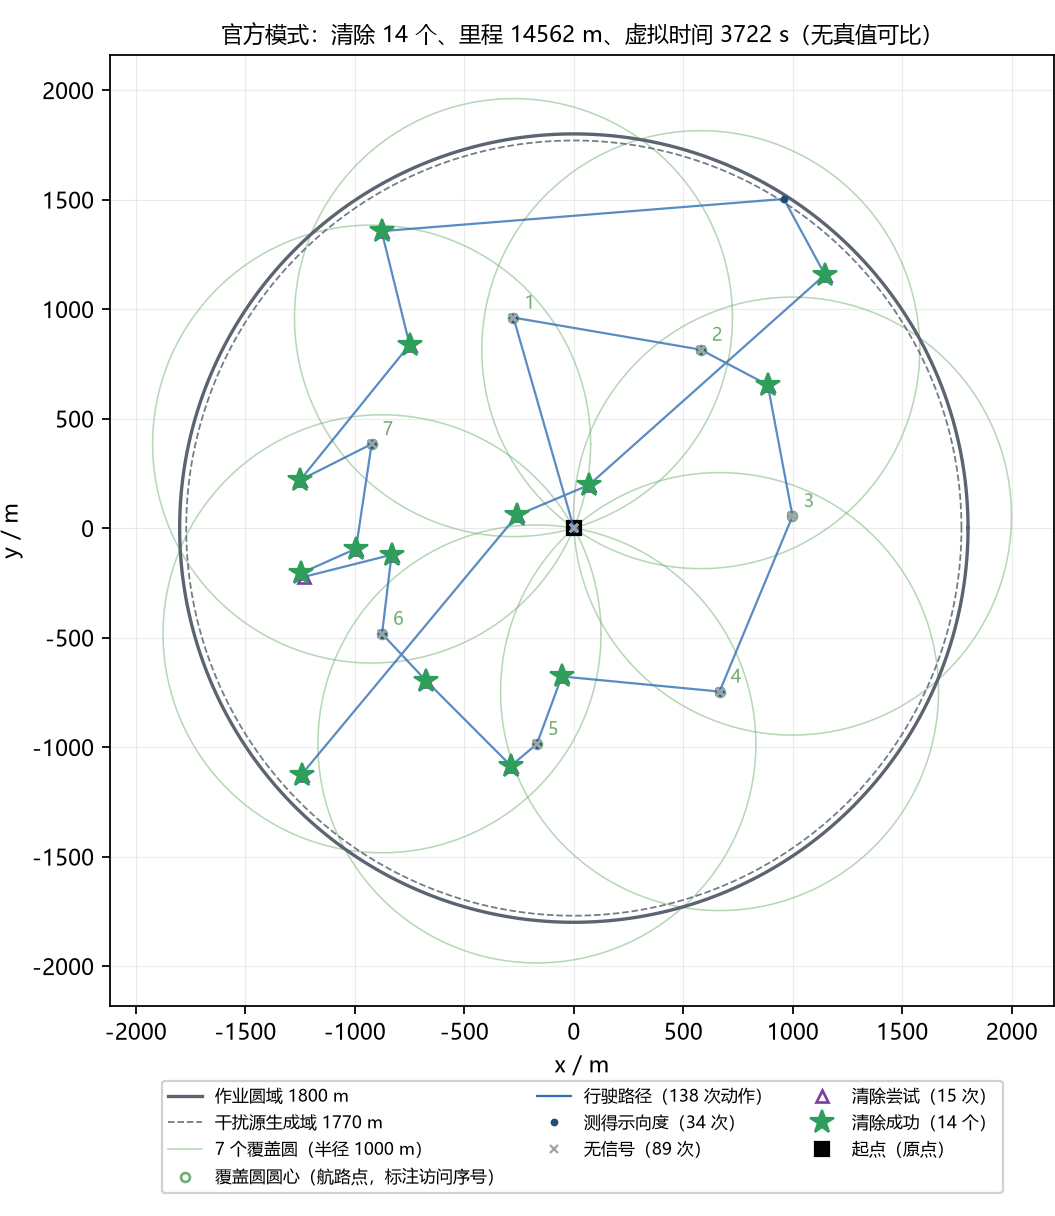
\includegraphics[width=0.5\textwidth]{figures/T3 14源.png}
  \caption{三次正式模拟（14 个干扰源）的全局行为图}
  \label{fig:three}
\end{figure}

\begin{figure}[H]
  \centering
  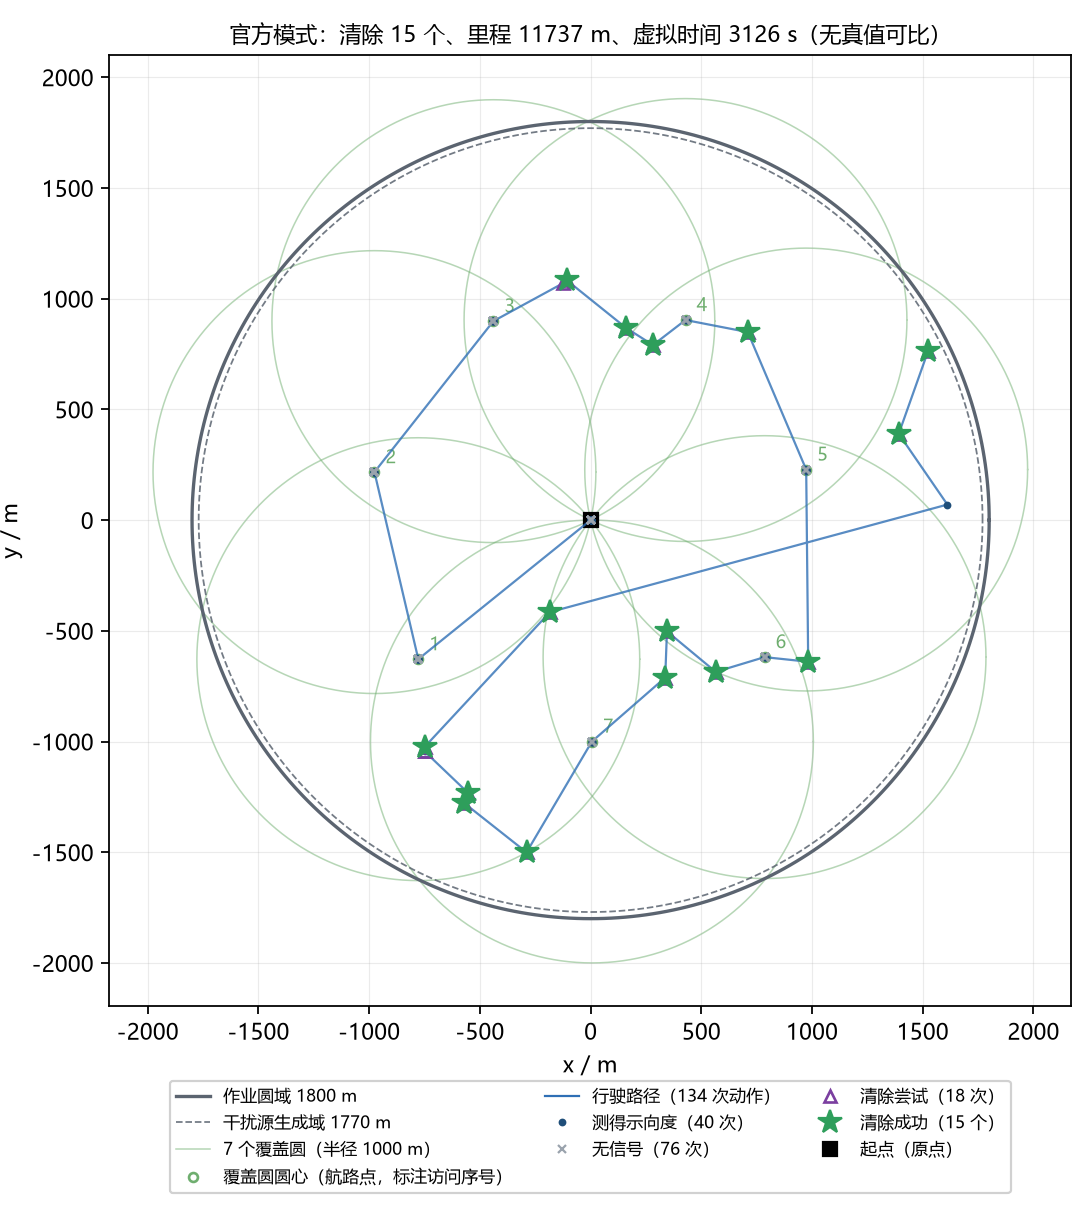
\includegraphics[width=0.5\textwidth]{figures/T3 15源.png}
  \caption{三次正式模拟（15 个干扰源）的全局行为图}
  \label{fig:three-b}
\end{figure}

\begin{figure}[H]
  \centering
  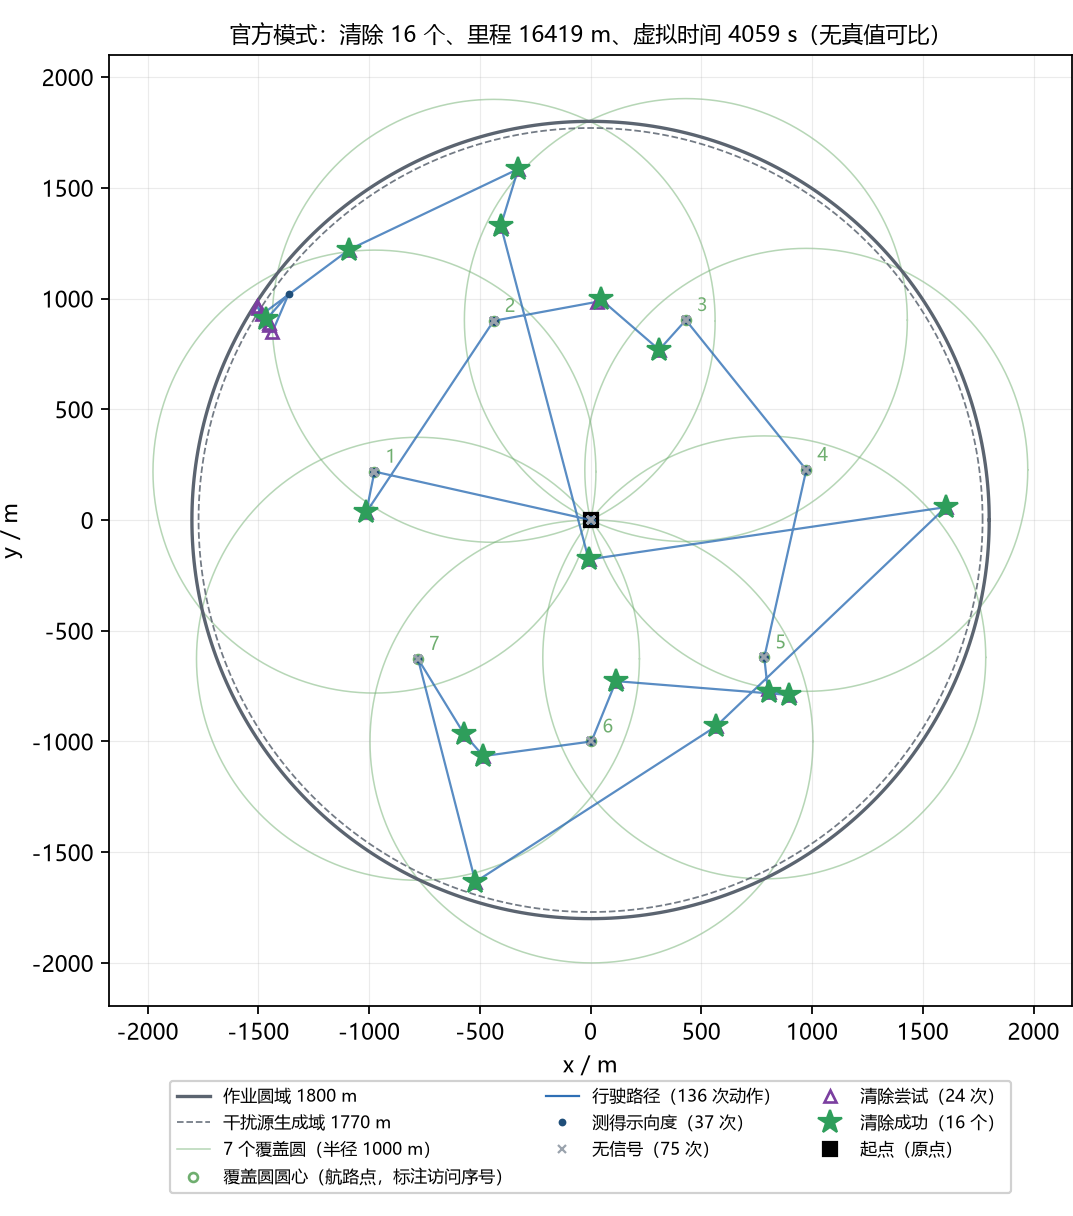
\includegraphics[width=0.5\textwidth]{figures/T3 16源.png}
  \caption{三次正式模拟（16 个干扰源）的全局行为图}
  \label{fig:three-c}
\end{figure}

\\begin{table}[H]
    \centering
    \caption{问题3正式测试结果}
    \begin{tabular}{cccc}
        \toprule
        测试案例编码 & 清除干扰源个数 & 平均定位清除时间 & 程序运行时间 \\
        \midrule
        测试1案例编码 & 14&265.883640 &3722.370961 \\
        测试2案例编码 &15 &208.426872 &3126.403078 \\
        测试3案例编码 & 16&253.676018 &4058.816295 \\
        \bottomrule
    \end{tabular}
\end{table}

\section*{七、  问题四模型建立及求解}
	\subsection*{7.1 模型建立}
	问题四引入了定向干扰源，其特性为仅在波束角 $\pm 90^{\circ}$（全角 $180^{\circ}$）内有信号，背光侧返回 \texttt{no\_signal}。这一物理特性导致问题三的策略失效：
\begin{itemize}
    \item 检测失效：问题三的 7 点覆盖仅保证“圆域内任意点到最近巡视点 $\le 1000\text{m}$”，对全向源必听到；但对定向源，背对所有巡视点的源即使距离极近也听不到（实测 7 点听到率仅 $80.7\%$）。
    \item 定位失效：问题三将 \texttt{no\_signal} 作为“源在检测点 1000m 外”的定位硬约束；问题四中 \texttt{no\_signal} 可能仅表示方向不对，不能转化为“圆盘外”约束。
\end{itemize}
因此，问题四需在未知源位置、未知波束方向、接收半径 $R \in [1000, 1500]\text{m}$ 的前提下，重新设计“检测—定位—清除”全流程，以清除率 $100\%$ 且虚拟总耗时最短为目标。

	\subsection*{7.2 检测与清除模型}
	\subsubsection*{7.2.1检测阶段：半圆盘命中模型}
定向源在测量点 $p$ 处可被听到，当且仅当满足距离与波束方向的双重约束：
\begin{equation}
|p - g| \le R \quad \text{且} \quad (p - g) \cdot u(\theta) \ge 0
\end{equation}
其中 $g$ 为源位置，$u(\theta) = (\cos\theta, \sin\theta)$ 为波束方向单位向量。即检测区是半径 $R$ 的半圆盘 $H(g, \theta, R)$，而 $g, \theta, R$ 全部未知。本文采用原点 + 7 覆盖基点 + 12 均匀方位外圈点（半径 $1850\text{m}$）的 20 点定案布局，确保对任意定向源至少有测量点落入其“迎光面”。

\subsubsection*{7.2.2定位阶段：硬约束交会模型}
听到某频道后，其定位区域由 \texttt{direction}（楔形与接收半径内包）与 \texttt{near}（距离 $\le 5\text{m}$）两类硬约束求交得到。\texttt{no\_signal} 一律不作为约束。补测点按示向度交会几何（Fisher信息度量）选取，使新射线尽量垂直于已有射线，以最大化缩小定位区域。

\subsubsection*{7.2.3清除阶段：三级递进清除机制}
\begin{itemize}
    \item 顺路清除：机器狗站间移动时，对“本站 $\to$ 下一站 $\to$ 圆心”夹出的方位扇区内的未清频道估计点顺路试清，命中节省时间，未中仅耗 $3\text{s}$。
    \item 就近试清：定位区域最小覆盖圆半径 $\le 400\text{m}$ 时直接试清；未中则用至多 $K=4$ 个半径 $20\text{m}$ 的圆覆盖定位区域逐点试清。
    \item 兜底逼近：沿示向度逐步逼近直至进入 $20\text{m}$ 清除半径，作为多视角交会失效时的保底手段。
\end{itemize}

	\subsection*{7.3模型求解}
	模型采用确定性算法求解，全程无随机数，同种子下逐字节可复现。
\begin{enumerate}
    \item 检测布局求解：采用最近邻 + 2-opt 局部搜索精修访问路线，外圈半径 $1850\text{m}$、方位间隔 $30^{\circ}$，访问总里程 $16995.65\text{m}$。
    \item 清除顺序调度：清除动作按“顺路清除 $\to$ 就近试清 $\to$ 兜底逼近”的优先级顺序进行调度，每个干扰源最多采集 4 条示向度（示向度条数上限为 4）。
    \item 时间优化：通过系统地旋钮探索（如顺路清除开关、外圈优先等），收敛到 $6444.8\text{s}$ 的实测时间下界。
\end{enumerate}
	\subsection*{7.4结果及分析}
	\subsubsection*{7.4.1算法结果}
基于本地模拟器（与官方引擎同判据）在 seed 0-19 的 20 局演练中（共 256 个干扰源），算法表现如下：

\\begin{table}[H]
\centering
\caption{20局演练汇总（seed 0-19，20点定案布局）}
\begin{tabular}{lcc}
\toprule
指标 & 数值 & 备注 \\
\midrule
清除比例 & $256/256 = 100\%$ & 20/20局全部清完，0失败 \\
平均定位清除时间 & $503.5\,\text{s/个}$ & 总虚拟时长 $\div$ 清除源数 \\
平均虚拟总耗时 & $6444.8\text{s}$ & $\approx 107\text{min}$，逐局 $5580 \sim 7861\text{s}$ \\
定位误差 & 均值 $7.66\text{m}$ & 最差 $19.67\text{m}$，全部 $\le 20\text{m}$ \\
\bottomrule
\end{tabular}
\end{table}

虚拟时长构成（总 $6444.8\text{s}$）：移动占约 $76\%$，测向占约 $19\%$，清除占约 $5\%$。前两项本质不可压缩，路径已逼近下界。

\subsubsection*{7.4.2统计验证与下界证明}
\begin{itemize}
    \item 听到率验证：422.5 万例全口径蒙特卡洛与对抗枚举校验显示，整体听到率达 $99.9891\%$，贴边对抗 0 漏（数据来源 \texttt{t4\_sweep\_plan.json} 的 \texttt{verify} 字段）。
    \item 时间下界：通过 2-20 局同 seed 对拍逐旋钮验证，确认 $6444.8\text{s}$ 为实测下界。神经网络独立搜索（遗传算法 + 代理模型）全部候选布局均更慢（如 23 点版 $6930\text{s}$，NN 12 外圈版 $7318\text{s}$），证伪了“存在更短耗时布局”的假设。
    \item 敏感性分析：外圈半径 $1850\text{m}$ 是贴边源与内部源迎光面覆盖的平衡点；12 个方位是减少绕路的实战极值；内部补点虽能微弱提升听率，但实测反而增加耗时。
\end{itemize}

\begin{figure}[H]
  \centering
  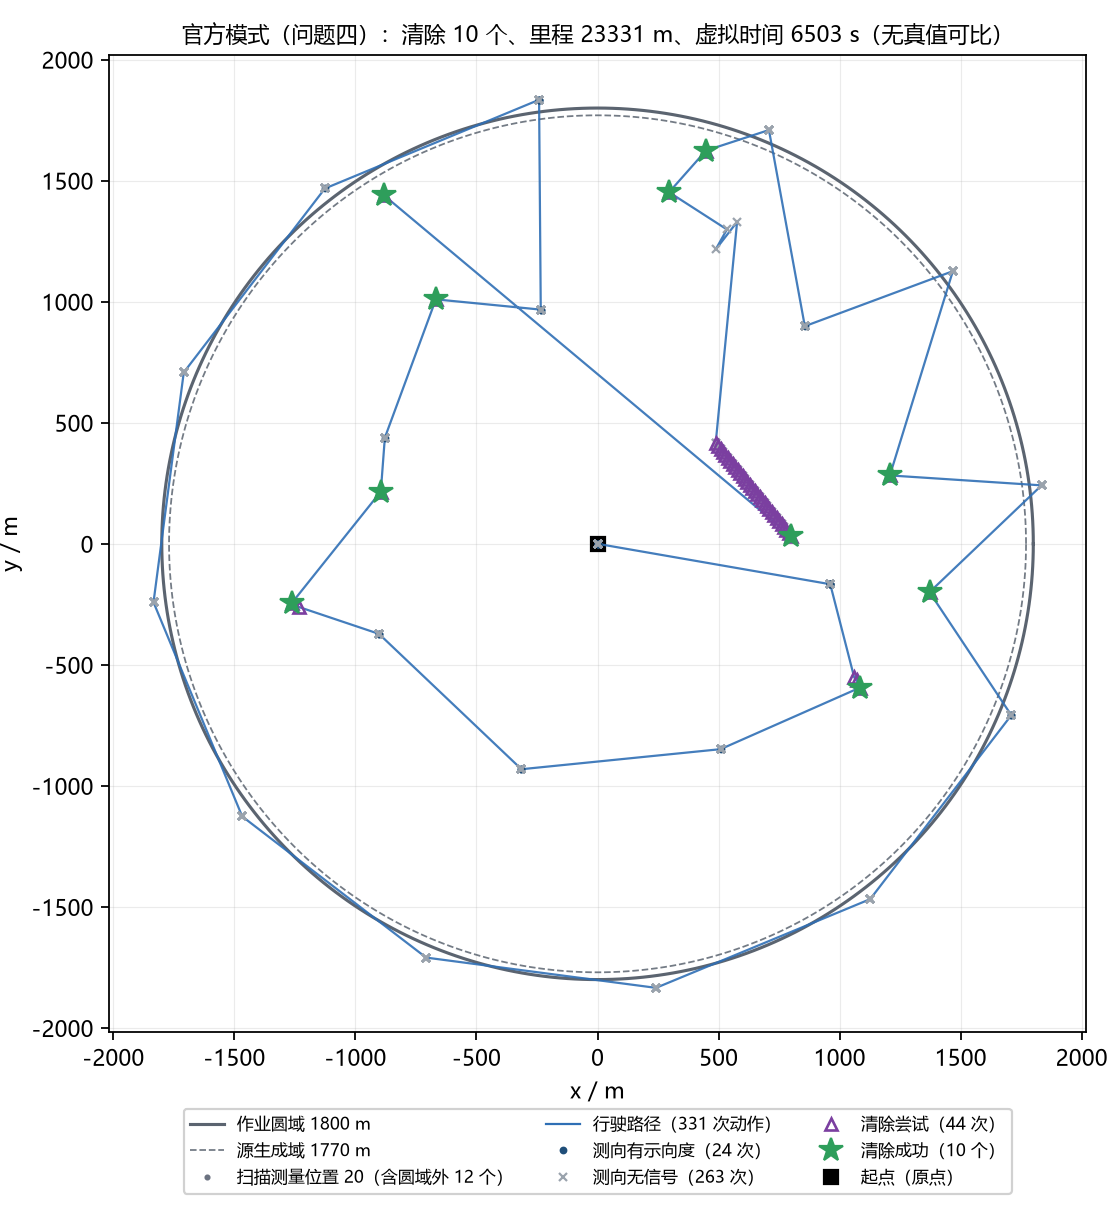
\includegraphics[width=0.5\textwidth]{figures/T4 10源.png}
  \caption{三次正式模拟（10 个干扰源）的全局行为图}
  \label{fig:four}
\end{figure}

\begin{figure}[H]
  \centering
  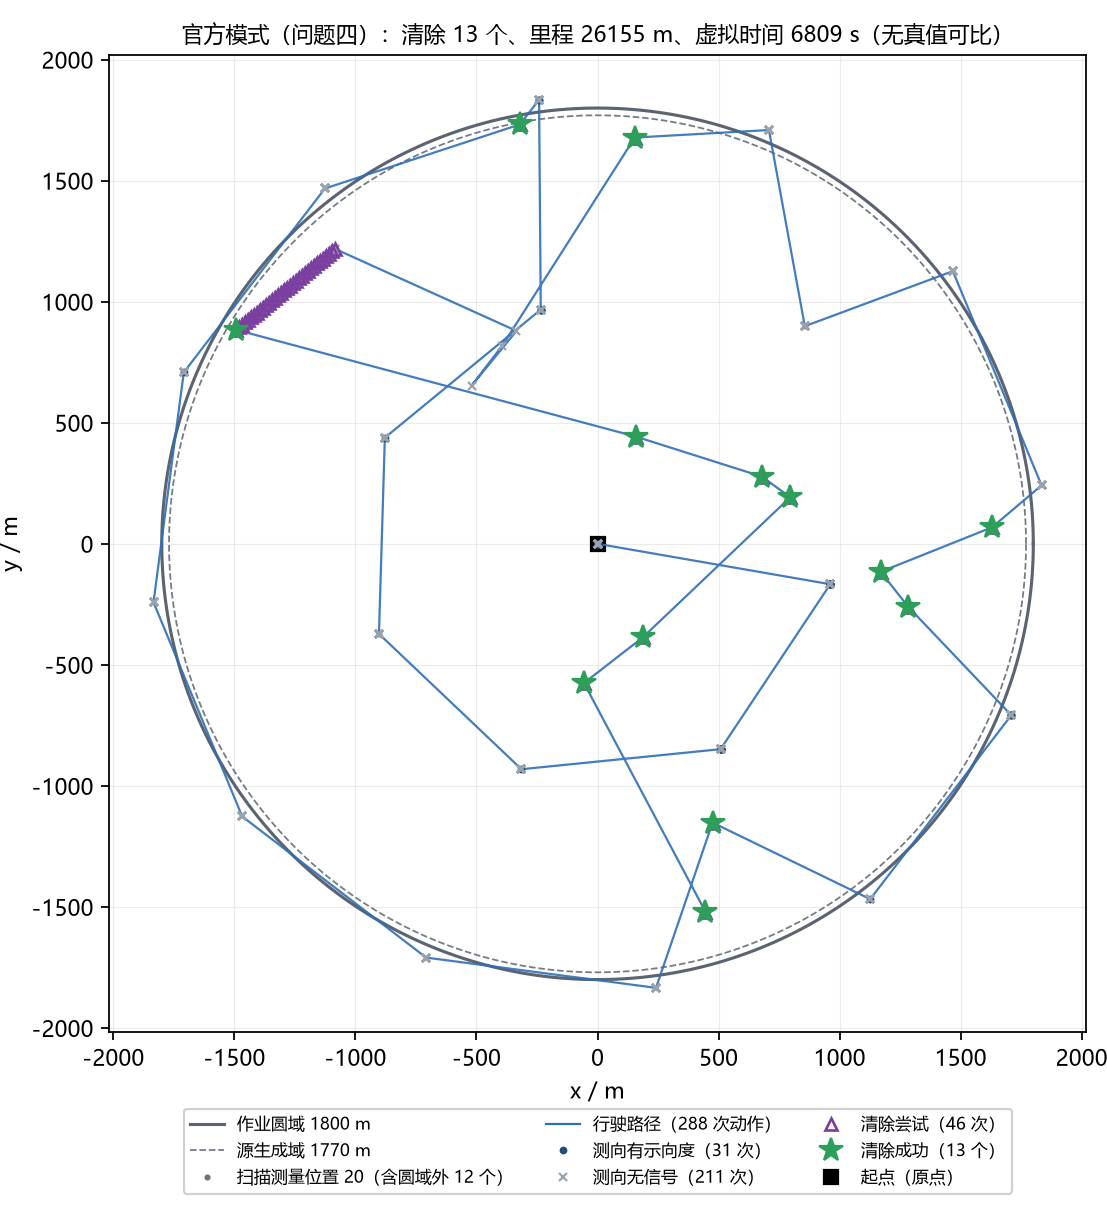
\includegraphics[width=0.5\textwidth]{figures/T4 13源.png}
  \caption{三次正式模拟（13 个干扰源）的全局行为图}
  \label{fig:four-b}
\end{figure}

\begin{figure}[H]
  \centering
  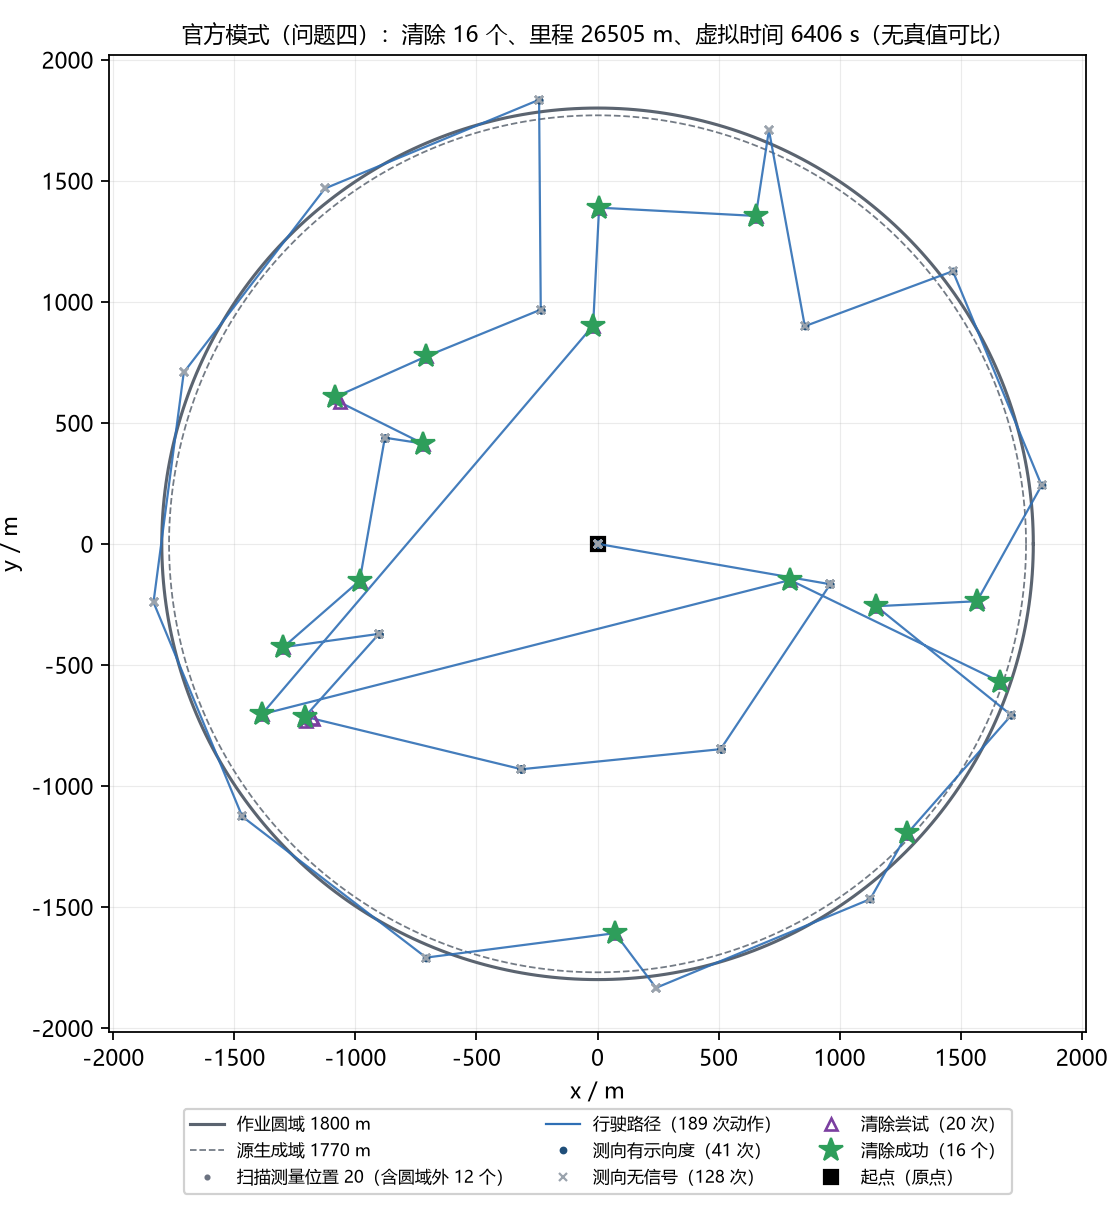
\includegraphics[width=0.5\textwidth]{figures/T4 16源.png}
  \caption{三次正式模拟（16 个干扰源）的全局行为图}
  \label{fig:four-c}
\end{figure}

\\begin{table}[H]
    \centering
    \caption{问题4正式测试结果}
    \begin{tabular}{cccc}
        \toprule
        测试案例编码 & 清除干扰源个数 & 平均定位清除时间 & 程序运行时间 \\
        \midrule
        测试1案例编码 & 16&400.373020 &6405.968326 \\
        测试2案例编码 &13 &523.775911 &6809.086039 \\
        测试3案例编码 &10 &650.32663 &6503.2663 \\
        \bottomrule
    \end{tabular}
\end{table}

% ---------- AI 工具使用声明（人工智能工具使用规定第 3 条：置于参考文献之前） ----------
% 论文里只出声明那一段；同一份 ai-declaration.tex 独立编译时出支撑材料要的《AI 工具使用详情》
%!TEX program = xelatex
% ---------------------------------------------------------------------------
% AI 工具使用声明（论文用）/ AI 工具使用详情（支撑材料用）
% 2026 年高教社杯全国大学生数学建模竞赛 B 题
%
% 依据《全国大学生数学建模竞赛人工智能工具使用规定（2026 年试行）》第 3、4 条：
% 论文参考文献之前要有"AI 工具使用声明"，内容二选一；用了 AI 的，还得在支撑材料里
% 放一份"AI工具使用详情.pdf"。规定原文：
% https://www.mcm.edu.cn/html_cn/node/fef94648f2836ab6cc81586f4c38512b.html
%
% 同一个文件两种用法，看编译方式自动切换，不用手工改：
%
%   独立编译   xelatex ai-declaration.tex
%              出《AI 工具使用详情》，就是支撑材料要的那份 PDF。交之前改名：
%                mv ai-declaration.pdf AI工具使用详情.pdf
%
%   论文引用   在论文"参考文献"之前写 %!TEX program = xelatex
% ---------------------------------------------------------------------------
% AI 工具使用声明（论文用）/ AI 工具使用详情（支撑材料用）
% 2026 年高教社杯全国大学生数学建模竞赛 B 题
%
% 依据《全国大学生数学建模竞赛人工智能工具使用规定（2026 年试行）》第 3、4 条：
% 论文参考文献之前要有"AI 工具使用声明"，内容二选一；用了 AI 的，还得在支撑材料里
% 放一份"AI工具使用详情.pdf"。规定原文：
% https://www.mcm.edu.cn/html_cn/node/fef94648f2836ab6cc81586f4c38512b.html
%
% 同一个文件两种用法，看编译方式自动切换，不用手工改：
%
%   独立编译   xelatex ai-declaration.tex
%              出《AI 工具使用详情》，就是支撑材料要的那份 PDF。交之前改名：
%                mv ai-declaration.pdf AI工具使用详情.pdf
%
%   论文引用   在论文"参考文献"之前写 %!TEX program = xelatex
% ---------------------------------------------------------------------------
% AI 工具使用声明（论文用）/ AI 工具使用详情（支撑材料用）
% 2026 年高教社杯全国大学生数学建模竞赛 B 题
%
% 依据《全国大学生数学建模竞赛人工智能工具使用规定（2026 年试行）》第 3、4 条：
% 论文参考文献之前要有"AI 工具使用声明"，内容二选一；用了 AI 的，还得在支撑材料里
% 放一份"AI工具使用详情.pdf"。规定原文：
% https://www.mcm.edu.cn/html_cn/node/fef94648f2836ab6cc81586f4c38512b.html
%
% 同一个文件两种用法，看编译方式自动切换，不用手工改：
%
%   独立编译   xelatex ai-declaration.tex
%              出《AI 工具使用详情》，就是支撑材料要的那份 PDF。交之前改名：
%                mv ai-declaration.pdf AI工具使用详情.pdf
%
%   论文引用   在论文"参考文献"之前写 \input{resources/latex/ai-declaration.tex}
%              只出标题和那一句话，详情表格自动跳过，正文不会违反第 3 条。
%              这段不依赖任何宏包，塞进哪个模板都行；想让标题带编号，把下面
%              \AIDeclHeading 里的 \section* 换成 \section。
%
% 交之前自己核一遍（第 5 条：假声明、瞒着不报会取消评奖资格）：
%   - 二选一跟实际对不对得上？本文件按"用了"填，没用 AI 的那句在下面注释里；
%   - "主要用于……"、工具名称与版本、使用环节、核验情况是不是本队真实情况？
%     详情表里没做过的行删掉；
%   - 论文和支撑材料里不能出现学校、赛区、队号，所以这里不写队号。
% ---------------------------------------------------------------------------

\makeatletter
% \@classoptionslist 是 \documentclass 定义的宏。文件开头它已经存在，就说明文档类加载过了，
% 也就是本文件正在被论文 \input，不是独立编译
\@ifundefined{ifAIDeclStandalone}{\newif\ifAIDeclStandalone}{}
\@ifundefined{@classoptionslist}{\AIDeclStandalonetrue}{\AIDeclStandalonefalse}
\ifAIDeclStandalone
  \documentclass[12pt,a4paper]{ctexart}
  \usepackage{geometry}
  \geometry{a4paper,left=2.6cm,right=2.6cm,top=2.6cm,bottom=2.6cm}
  \usepackage{booktabs}
  \usepackage{array}
  \usepackage{xeCJK}
  \linespread{1.3}
  \pagestyle{empty}                         % 支撑材料附件不要页码
\fi
\makeatother

% 规程第 3 条要的那句话。两种用法共用，改这里两边同步。
\providecommand{\AIDeclSentence}{%
  本参赛队在竞赛过程中使用了AI工具，主要用于代码编写与调试、模型方案比选与%
  数值结果核验、图表与文字整理及语言润色，详细使用情况见支撑材料。%
}
% 没用 AI 就换成下面这句，并把详情表格和后面几节一并删掉：
% \providecommand{\AIDeclSentence}{本参赛队在竞赛过程中未使用任何AI工具。}

\ifAIDeclStandalone
% 独立编译：出支撑材料用的《AI 工具使用详情》，覆盖规程第 4 条的四项内容
\begin{document}

\begin{center}
  {\zihao{3}\bfseries AI 工具使用详情}\\[0.6em]
\end{center}

\subsection*{一、声明}

\AIDeclSentence

\subsection*{二、所用 AI 工具的名称、版本或型号}

\begin{table}[htbp]
  \centering
  \begin{tabular}{@{}p{5.0cm}p{3.5cm}p{6.45cm}@{}}
    \toprule
    工具名称 & 版本 / 型号 & 使用环节 \\
    \midrule
    DeepSeek Harness 智能体 & deepseek-v4-flash &
      建模推导草案、求解代码编写与调试、数值结果复核、图表与文字整理 \\
    \bottomrule
  \end{tabular}
\end{table}

% 本队还用过别的工具就照上面的格式加行，没有就保持原样
\noindent\emph{注：除上表所列工具外，本队未使用其他 AI 工具。}

\subsection*{三、具体使用目的和环节}

\begin{table}[htbp]
  \centering
  \begin{tabular}{@{}p{3.0cm}p{5.2cm}p{6.75cm}@{}}
    \toprule
    环节 & 使用目的 & 采纳情况 \\
    \midrule
    赛题理解与建模设计 &
      梳理子问题、提出可行模型（测向交会定位、最坏情形定位误差、覆盖圆搜索、多源扫描计划）作为讨论草案 &
      部分采纳：模型假设、目标函数与判据由参赛队确定 \\
    \addlinespace
    求解代码实现 &
      生成几何计算、覆盖圆布局、批量扫描判据等代码骨架 &
      采纳后逐行修改：几何裁剪方式、最少覆盖圆选向等不符合题意的部分由参赛队改写 \\
    \addlinespace
    结果核验与复现 &
      编写模块自检脚本、固定随机种子的复现脚本 &
      采纳：用作参赛队核验结果的辅助手段 \\
    \addlinespace
    图表与论文撰写 &
      绘制数据图、整理表格与图注、语言润色 &
      采纳：仅整理表述与排版，不改变数据与结论 \\
    \bottomrule
  \end{tabular}
\end{table}

\subsection*{四、主要提示方式与使用过程说明}

提示一律用自然语言，把题目条件、精度要求和必须可复现这些约束一次说清；同时要求给出推导过程
和\emph{可运行}的代码，不接受只有结论的描述。关键判断上再追问一轮，让它自查，或者要求批量实现
与单例参考逐元素对齐，免得拿到"看着对但核不动"的东西。

两个有代表性的例子：

\begin{itemize}
  \item 问题三的覆盖圆。提示："作业区里每个干扰源都必须落在某个覆盖圆内，给出覆盖圆数量最少
    的方案，并说明旋转与选向怎么取舍。"返回的方案与代码可用，但参赛队核对"作业区边界截断"
    的确切含义后，改掉了最少覆盖圆数的判定。
  \item 批量命中判定。提示："把命中判定改成批量实现，要求每个元素与单例参考做完全相同的浮点
    运算，结果逐字节一致。"拿到实现后，先用自检脚本比对批量与单例，再跑一遍演练，确认一致
    才采纳。
\end{itemize}

\subsection*{五、对 AI 输出的采纳、人工修改和核验的主要情况}

采纳的部分：推导草案、代码骨架、自检脚本，以及文档与语言润色。

人工修改的部分：模型假设、几何构造、判据与参数取值都由参赛队确定；AI 给出的代码逐行读过，
不符合题意的地方（几何裁剪方式、覆盖圆选向规则、扫描点排布等）都作了改写。

核验做了四件事：

\begin{enumerate}
  \item 全部求解代码在本机重新运行，模块自检脚本逐项通过：几何构造与解析解对比、文献判据
    对比、覆盖方案检查、批量实现与单例参考对比、静态检查；
  \item 关键结果以固定随机种子重复运行，重复运行的产物与论文、附录中的数据一致；产物位于
    \texttt{results/}，删除后重跑即可重建；
  \item 论文中的公式、数据与结论逐项与程序输出核对，不一致处以程序输出为准；
  \item 语言润色与文字整理只调整表述，没有改动任何数据与结论。
\end{enumerate}

\end{document}

\else
% 论文模式：只出规程第 3 条要求的"AI 工具使用声明"小节
\providecommand{\AIDeclHeading}[1]{\section*{#1}}% 需要编号时改为 \section
\AIDeclHeading{AI 工具使用声明}

\AIDeclSentence

\fi

%              只出标题和那一句话，详情表格自动跳过，正文不会违反第 3 条。
%              这段不依赖任何宏包，塞进哪个模板都行；想让标题带编号，把下面
%              \AIDeclHeading 里的 \section* 换成 \section。
%
% 交之前自己核一遍（第 5 条：假声明、瞒着不报会取消评奖资格）：
%   - 二选一跟实际对不对得上？本文件按"用了"填，没用 AI 的那句在下面注释里；
%   - "主要用于……"、工具名称与版本、使用环节、核验情况是不是本队真实情况？
%     详情表里没做过的行删掉；
%   - 论文和支撑材料里不能出现学校、赛区、队号，所以这里不写队号。
% ---------------------------------------------------------------------------

\makeatletter
% \@classoptionslist 是 \documentclass 定义的宏。文件开头它已经存在，就说明文档类加载过了，
% 也就是本文件正在被论文 \input，不是独立编译
\@ifundefined{ifAIDeclStandalone}{\newif\ifAIDeclStandalone}{}
\@ifundefined{@classoptionslist}{\AIDeclStandalonetrue}{\AIDeclStandalonefalse}
\ifAIDeclStandalone
  \documentclass[12pt,a4paper]{ctexart}
  \usepackage{geometry}
  \geometry{a4paper,left=2.6cm,right=2.6cm,top=2.6cm,bottom=2.6cm}
  \usepackage{booktabs}
  \usepackage{array}
  \usepackage{xeCJK}
  \linespread{1.3}
  \pagestyle{empty}                         % 支撑材料附件不要页码
\fi
\makeatother

% 规程第 3 条要的那句话。两种用法共用，改这里两边同步。
\providecommand{\AIDeclSentence}{%
  本参赛队在竞赛过程中使用了AI工具，主要用于代码编写与调试、模型方案比选与%
  数值结果核验、图表与文字整理及语言润色，详细使用情况见支撑材料。%
}
% 没用 AI 就换成下面这句，并把详情表格和后面几节一并删掉：
% \providecommand{\AIDeclSentence}{本参赛队在竞赛过程中未使用任何AI工具。}

\ifAIDeclStandalone
% 独立编译：出支撑材料用的《AI 工具使用详情》，覆盖规程第 4 条的四项内容
\begin{document}

\begin{center}
  {\zihao{3}\bfseries AI 工具使用详情}\\[0.6em]
\end{center}

\subsection*{一、声明}

\AIDeclSentence

\subsection*{二、所用 AI 工具的名称、版本或型号}

\begin{table}[htbp]
  \centering
  \begin{tabular}{@{}p{5.0cm}p{3.5cm}p{6.45cm}@{}}
    \toprule
    工具名称 & 版本 / 型号 & 使用环节 \\
    \midrule
    DeepSeek Harness 智能体 & deepseek-v4-flash &
      建模推导草案、求解代码编写与调试、数值结果复核、图表与文字整理 \\
    \bottomrule
  \end{tabular}
\end{table}

% 本队还用过别的工具就照上面的格式加行，没有就保持原样
\noindent\emph{注：除上表所列工具外，本队未使用其他 AI 工具。}

\subsection*{三、具体使用目的和环节}

\begin{table}[htbp]
  \centering
  \begin{tabular}{@{}p{3.0cm}p{5.2cm}p{6.75cm}@{}}
    \toprule
    环节 & 使用目的 & 采纳情况 \\
    \midrule
    赛题理解与建模设计 &
      梳理子问题、提出可行模型（测向交会定位、最坏情形定位误差、覆盖圆搜索、多源扫描计划）作为讨论草案 &
      部分采纳：模型假设、目标函数与判据由参赛队确定 \\
    \addlinespace
    求解代码实现 &
      生成几何计算、覆盖圆布局、批量扫描判据等代码骨架 &
      采纳后逐行修改：几何裁剪方式、最少覆盖圆选向等不符合题意的部分由参赛队改写 \\
    \addlinespace
    结果核验与复现 &
      编写模块自检脚本、固定随机种子的复现脚本 &
      采纳：用作参赛队核验结果的辅助手段 \\
    \addlinespace
    图表与论文撰写 &
      绘制数据图、整理表格与图注、语言润色 &
      采纳：仅整理表述与排版，不改变数据与结论 \\
    \bottomrule
  \end{tabular}
\end{table}

\subsection*{四、主要提示方式与使用过程说明}

提示一律用自然语言，把题目条件、精度要求和必须可复现这些约束一次说清；同时要求给出推导过程
和\emph{可运行}的代码，不接受只有结论的描述。关键判断上再追问一轮，让它自查，或者要求批量实现
与单例参考逐元素对齐，免得拿到"看着对但核不动"的东西。

两个有代表性的例子：

\begin{itemize}
  \item 问题三的覆盖圆。提示："作业区里每个干扰源都必须落在某个覆盖圆内，给出覆盖圆数量最少
    的方案，并说明旋转与选向怎么取舍。"返回的方案与代码可用，但参赛队核对"作业区边界截断"
    的确切含义后，改掉了最少覆盖圆数的判定。
  \item 批量命中判定。提示："把命中判定改成批量实现，要求每个元素与单例参考做完全相同的浮点
    运算，结果逐字节一致。"拿到实现后，先用自检脚本比对批量与单例，再跑一遍演练，确认一致
    才采纳。
\end{itemize}

\subsection*{五、对 AI 输出的采纳、人工修改和核验的主要情况}

采纳的部分：推导草案、代码骨架、自检脚本，以及文档与语言润色。

人工修改的部分：模型假设、几何构造、判据与参数取值都由参赛队确定；AI 给出的代码逐行读过，
不符合题意的地方（几何裁剪方式、覆盖圆选向规则、扫描点排布等）都作了改写。

核验做了四件事：

\begin{enumerate}
  \item 全部求解代码在本机重新运行，模块自检脚本逐项通过：几何构造与解析解对比、文献判据
    对比、覆盖方案检查、批量实现与单例参考对比、静态检查；
  \item 关键结果以固定随机种子重复运行，重复运行的产物与论文、附录中的数据一致；产物位于
    \texttt{results/}，删除后重跑即可重建；
  \item 论文中的公式、数据与结论逐项与程序输出核对，不一致处以程序输出为准；
  \item 语言润色与文字整理只调整表述，没有改动任何数据与结论。
\end{enumerate}

\end{document}

\else
% 论文模式：只出规程第 3 条要求的"AI 工具使用声明"小节
\providecommand{\AIDeclHeading}[1]{\section*{#1}}% 需要编号时改为 \section
\AIDeclHeading{AI 工具使用声明}

\AIDeclSentence

\fi

%              只出标题和那一句话，详情表格自动跳过，正文不会违反第 3 条。
%              这段不依赖任何宏包，塞进哪个模板都行；想让标题带编号，把下面
%              \AIDeclHeading 里的 \section* 换成 \section。
%
% 交之前自己核一遍（第 5 条：假声明、瞒着不报会取消评奖资格）：
%   - 二选一跟实际对不对得上？本文件按"用了"填，没用 AI 的那句在下面注释里；
%   - "主要用于……"、工具名称与版本、使用环节、核验情况是不是本队真实情况？
%     详情表里没做过的行删掉；
%   - 论文和支撑材料里不能出现学校、赛区、队号，所以这里不写队号。
% ---------------------------------------------------------------------------

\makeatletter
% \@classoptionslist 是 \documentclass 定义的宏。文件开头它已经存在，就说明文档类加载过了，
% 也就是本文件正在被论文 \input，不是独立编译
\@ifundefined{ifAIDeclStandalone}{\newif\ifAIDeclStandalone}{}
\@ifundefined{@classoptionslist}{\AIDeclStandalonetrue}{\AIDeclStandalonefalse}
\ifAIDeclStandalone
  \documentclass[12pt,a4paper]{ctexart}
  \usepackage{geometry}
  \geometry{a4paper,left=2.6cm,right=2.6cm,top=2.6cm,bottom=2.6cm}
  \usepackage{booktabs}
  \usepackage{array}
  \usepackage{xeCJK}
  \linespread{1.3}
  \pagestyle{empty}                         % 支撑材料附件不要页码
\fi
\makeatother

% 规程第 3 条要的那句话。两种用法共用，改这里两边同步。
\providecommand{\AIDeclSentence}{%
  本参赛队在竞赛过程中使用了AI工具，主要用于代码编写与调试、模型方案比选与%
  数值结果核验、图表与文字整理及语言润色，详细使用情况见支撑材料。%
}
% 没用 AI 就换成下面这句，并把详情表格和后面几节一并删掉：
% \providecommand{\AIDeclSentence}{本参赛队在竞赛过程中未使用任何AI工具。}

\ifAIDeclStandalone
% 独立编译：出支撑材料用的《AI 工具使用详情》，覆盖规程第 4 条的四项内容
\begin{document}

\begin{center}
  {\zihao{3}\bfseries AI 工具使用详情}\\[0.6em]
\end{center}

\subsection*{一、声明}

\AIDeclSentence

\subsection*{二、所用 AI 工具的名称、版本或型号}

\begin{table}[htbp]
  \centering
  \begin{tabular}{@{}p{5.0cm}p{3.5cm}p{6.45cm}@{}}
    \toprule
    工具名称 & 版本 / 型号 & 使用环节 \\
    \midrule
    DeepSeek Harness 智能体 & deepseek-v4-flash &
      建模推导草案、求解代码编写与调试、数值结果复核、图表与文字整理 \\
    \bottomrule
  \end{tabular}
\end{table}

% 本队还用过别的工具就照上面的格式加行，没有就保持原样
\noindent\emph{注：除上表所列工具外，本队未使用其他 AI 工具。}

\subsection*{三、具体使用目的和环节}

\begin{table}[htbp]
  \centering
  \begin{tabular}{@{}p{3.0cm}p{5.2cm}p{6.75cm}@{}}
    \toprule
    环节 & 使用目的 & 采纳情况 \\
    \midrule
    赛题理解与建模设计 &
      梳理子问题、提出可行模型（测向交会定位、最坏情形定位误差、覆盖圆搜索、多源扫描计划）作为讨论草案 &
      部分采纳：模型假设、目标函数与判据由参赛队确定 \\
    \addlinespace
    求解代码实现 &
      生成几何计算、覆盖圆布局、批量扫描判据等代码骨架 &
      采纳后逐行修改：几何裁剪方式、最少覆盖圆选向等不符合题意的部分由参赛队改写 \\
    \addlinespace
    结果核验与复现 &
      编写模块自检脚本、固定随机种子的复现脚本 &
      采纳：用作参赛队核验结果的辅助手段 \\
    \addlinespace
    图表与论文撰写 &
      绘制数据图、整理表格与图注、语言润色 &
      采纳：仅整理表述与排版，不改变数据与结论 \\
    \bottomrule
  \end{tabular}
\end{table}

\subsection*{四、主要提示方式与使用过程说明}

提示一律用自然语言，把题目条件、精度要求和必须可复现这些约束一次说清；同时要求给出推导过程
和\emph{可运行}的代码，不接受只有结论的描述。关键判断上再追问一轮，让它自查，或者要求批量实现
与单例参考逐元素对齐，免得拿到"看着对但核不动"的东西。

两个有代表性的例子：

\begin{itemize}
  \item 问题三的覆盖圆。提示："作业区里每个干扰源都必须落在某个覆盖圆内，给出覆盖圆数量最少
    的方案，并说明旋转与选向怎么取舍。"返回的方案与代码可用，但参赛队核对"作业区边界截断"
    的确切含义后，改掉了最少覆盖圆数的判定。
  \item 批量命中判定。提示："把命中判定改成批量实现，要求每个元素与单例参考做完全相同的浮点
    运算，结果逐字节一致。"拿到实现后，先用自检脚本比对批量与单例，再跑一遍演练，确认一致
    才采纳。
\end{itemize}

\subsection*{五、对 AI 输出的采纳、人工修改和核验的主要情况}

采纳的部分：推导草案、代码骨架、自检脚本，以及文档与语言润色。

人工修改的部分：模型假设、几何构造、判据与参数取值都由参赛队确定；AI 给出的代码逐行读过，
不符合题意的地方（几何裁剪方式、覆盖圆选向规则、扫描点排布等）都作了改写。

核验做了四件事：

\begin{enumerate}
  \item 全部求解代码在本机重新运行，模块自检脚本逐项通过：几何构造与解析解对比、文献判据
    对比、覆盖方案检查、批量实现与单例参考对比、静态检查；
  \item 关键结果以固定随机种子重复运行，重复运行的产物与论文、附录中的数据一致；产物位于
    \texttt{results/}，删除后重跑即可重建；
  \item 论文中的公式、数据与结论逐项与程序输出核对，不一致处以程序输出为准；
  \item 语言润色与文字整理只调整表述，没有改动任何数据与结论。
\end{enumerate}

\end{document}

\else
% 论文模式：只出规程第 3 条要求的"AI 工具使用声明"小节
\providecommand{\AIDeclHeading}[1]{\section*{#1}}% 需要编号时改为 \section
\AIDeclHeading{AI 工具使用声明}

\AIDeclSentence

\fi


% ---------- 参考文献 ----------
\newpage
\begin{thebibliography}{99}
    
	\bibitem{zhao2012} ZHAO S, CHEN B M, LEE T H. Optimal placement of bearing-only sensors for target localization[C]//2012 American Control Conference (ACC). Montreal: IEEE, 2012: 5108--5113.
    \bibitem{Gaspar2021} GÁSPÁR Z, TARNAI T, HINCZ K. Partial Covering of a Circle by 6 and 7 Congruent Circles[J]. Symmetry, 2021, 13(11): 2133.

	\bibitem{renyetong} 任叶童. 基于到达角信息的无源定位算法研究[D]. 南京: 南京邮电大学, 2019.

	\bibitem{liaohaijun} 廖海军. 多站无源定位精度分析及相关技术研究[D]. 成都: 电子科技大学, 2008.

	\bibitem{guoyongning} 郭永宁. 无人机无线电监测混合定位算法[J]. 桂林电子科技大学学报, 2021, 41(5): 351--356.

	\bibitem{wangqi} 王琦, 吕云飞, 兰华林, 等. 双矢量潜标被动定位方法研究[J]. 声学技术, 2016, 35(3): 216--220.

	\bibitem{yinzan} 殷赞. 卫星导航多干扰源测向定位技术及应用[J]. 全球定位系统, 2023, 48(1): 1--8.

\end{thebibliography}

\section*{附录}

	\noindent 附录收录四个问题从读入测量到给出答案的求解逻辑：问题一的定位区域求交，问题二的源不确定集采样、最坏定位直径与候选区域，问题三、四的覆盖布局、可能源集合的硬约束叠加、补测选点与巡视清除策略。命令行解析、绘图、报告输出、模块自检与模拟器接口封装（common/sim\_client.py）不在附录内，完整工程代码见支撑材料。代码中出现的圆域半径、覆盖半径、采样格数等常数集中定义在各问题的 config 模块里。

\subsection*{附录 A \quad 问题一：交会定位区域的求交与几何量}

	\noindent 问题一把每条示向度展开成张角 $2\varepsilon$ 的楔形，检测点逐个与目标圆域求交，再从交出的凸多边形上量直径、最小覆盖圆与是否被圆域截断。下面是一个检测点集合求交与量测的完整实现。

	\subsubsection*{A.1 \quad 定位区域类（t1/triangulation.py）}
	\begin{lstlisting}
class TriangulationRegion:
    """交会定位区域：累积检测点后求定位区域凸多边形及其几何量"""

    RADIUS = 1800.0  # 目标圆域半径（米），题目给定（直径 3600 m）
    SIDES = 64       # 目标圆域的内接正多边形边数，须为 4 的倍数
    TOUCH = 1.0      # 顶点贴合圆域边界的判定阈值（米）

    def __init__(self, err: float = 1.0, radius: float | None = None, sides: int | None = None) -> None:
        """构造交会定位区域，err 为示向度误差半宽（度）"""
        self.err = float(err)
        self.radius = self.RADIUS if radius is None else float(radius)
        self.sides = self.SIDES if sides is None else int(sides)
        if self.sides % 4:
            raise ValueError("sides 必须是 4 的倍数")
        self._nodes = []
        self._clip = None    # 目标圆域的内接正多边形（惰性生成）
        self._region = None  # 已并入前 _done 个检测点的交集；None 表示尚未求解
        self._done = 0

    # ---------- 检测点管理 ----------

    def add_node(self, x: float, y: float, theta: float) -> TriangulationRegion:
        """加入一个检测点，坐标为米、示向度为度，返回自身便于链式调用"""
        self._nodes.append((float(x), float(y), float(theta) % 360.0))
        return self

    @classmethod
    def from_nodes(cls, nodes: list[tuple[float, float, float]], err: float = 1.0,
                   radius: float | None = None, sides: int | None = None) -> TriangulationRegion:
        """由检测点列表 [(x, y, theta), ...] 构造定位区域，坐标为米、示向度为度"""
        region = cls(err, radius, sides)
        for x, y, theta in nodes:
            region.add_node(x, y, theta)
        return region

    # ---------- 定位区域与几何量 ----------

    @property
    def clip(self) -> Polygon:
        """目标圆域，也就是内接正 sides 边形，顶点精确落在半径 radius 的圆上"""
        if self._clip is None:
            self._clip = Point(0.0, 0.0).buffer(self.radius, quad_segs=self.sides // 4)
        return self._clip

    @property
    def region(self) -> Polygon:
        """定位区域的 shapely 几何，空区域返回空几何"""
        if self._region is None:
            # 楔形张角为 0，也就是 err<=0 时，区域退化成零面积
            self._region = self.clip if self.err > 0.0 else Polygon()
            self._done = 0
        for x, y, theta in self._nodes[self._done:]:
            self._region = self._region.intersection(self._wedge(x, y, theta))
            self._done += 1
            if self._region.is_empty:  # 空区域与任何楔形相交仍为空
                self._done = len(self._nodes)
                break
        return self._region

    @property
    def vertices(self) -> list[tuple[float, float]]:
        """定位区域顶点坐标列表 [(x, y), ...]，统一成逆时针，空区域返回空表"""
        region = self.region
        if region.is_empty or region.geom_type != "Polygon":
            return []
        pts = [(x, y) for x, y, *_ in region.exterior.coords[:-1]]
        return pts if region.exterior.is_ccw else pts[::-1]

    @property
    def area(self) -> float:
        """定位区域面积 / m²"""
        return float(self.region.area)

    @property
    def diameter(self) -> float:
        """定位区域直径：区域内任意两点距离的最大值 / m"""
        pts = np.asarray(self.vertices, dtype=float)
        if len(pts) < 2:
            return 0.0
        return float(np.linalg.norm(pts[:, None, :] - pts[None, :, :], axis=-1).max())

    @property
    def bounded(self) -> bool:
        """定位是否只靠检测点就已确定，没被目标圆域截断"""
        # 有顶点落在圆域边界上，说明那个方向约束不足
        pts = self.vertices
        return bool(pts) and all(self.clip.exterior.distance(Point(*p)) > self.TOUCH for p in pts)

    @property
    def enclosing_circle(self) -> tuple[float, float, float] | None:
        """定位区域的最小覆盖圆 (cx, cy, r) / m，区域为空或退化时返回 None"""
        # 问题 1 第二问的判据（以区域直径为直径的圆能否盖住区域）就是看 r <= diameter / 2
        if not self.vertices:
            return None
        # 最小包围圆是正内接多边形，它的质心就是圆心
        center = shapely.minimum_bounding_circle(self.region).centroid
        return (center.x, center.y, float(shapely.minimum_bounding_radius(self.region)))

    def contains(self, p: tuple[float, float]) -> bool:
        """点 p 是否落在定位区域内，圆域按内接多边形算，圆边上的月牙不算"""
        return bool(self.region.covers(Point(p)))

    # ---------- 基础几何 ----------

    def _wedge(self, x: float, y: float, theta: float) -> Polygon:
        """单个检测点的楔形多边形，以 (x, y) 为顶点，边长足够覆盖整个目标圆域"""
        length = 2.0 * (hypot(x, y) + self.radius)
        a1, a2 = radians(theta - self.err), radians(theta + self.err)
        return Polygon([(x, y),
                        (x + length * cos(a1), y + length * sin(a1)),
                        (x + length * cos(a2), y + length * sin(a2))])

    @staticmethod
    def bearing(a: tuple[float, float], b: tuple[float, float]) -> float:
        """a 点观测 b 点的方位角 / 度，x 轴正向逆时针为正，取值 [0, 360)"""
        return degrees(atan2(b[1] - a[1], b[0] - a[0])) % 360.0

    def __repr__(self) -> str:
        """对象的可读表示，汇总检测点数、顶点数、直径与 bounded"""
        return (f"TriangulationRegion(检测点 {len(self._nodes)} 个, 顶点 {len(self.vertices)} 个, "
                f"直径 {self.diameter:.4f} m, 仅靠检测点可确定 {self.bounded})")
	\end{lstlisting}

\subsection*{附录 B \quad 问题二：第二检测点的最坏定位直径寻优}

	\noindent 问题二在源不确定集 $\mathcal{C}$ 与第二次测向误差上取最坏情形，把最坏定位直径 $J(S_2)$ 作为目标函数：先采样源不确定集，在全域粗网格上算出每个候选点的 $J$，再在粗解附近细化，与文献判据（GDOP、CRLB、极小极大半径）的推荐落点对照，最后按 $J\le(1+\eta)J^*$ 给出候选区域弧带。

	\subsubsection*{B.1 \quad 两楔形之交的候选顶点与定位直径（t2/region.py）}
	\begin{lstlisting}
def _candidate_points_batch(site: Sequence[float], theta1: float, sx: np.ndarray, sy: np.ndarray,
                            theta2_batch: np.ndarray,
                            err_deg: float) -> tuple[np.ndarray, np.ndarray]:
    """一批楔形方向下两楔形之交的候选顶点 P (6, B, N, 2) 与在两楔形内的掩码 keep"""
    x1, y1 = float(site[0]), float(site[1])
    sx = np.asarray(sx, dtype=float)
    sy = np.asarray(sy, dtype=float)
    theta2_batch = np.asarray(theta2_batch, dtype=float)
    shape = theta2_batch.shape
    wx = np.broadcast_to(sx, shape) - x1
    wy = np.broadcast_to(sy, shape) - y1
    pts = []
    # θ₂ ± err 的单位向量只算一次。原先 (sa, sb) 四个组合各算一遍，其中两个重复
    bs = (_cos_sin(theta2_batch - err_deg), _cos_sin(theta2_batch + err_deg))
    for sa in (-err_deg, err_deg):
        ax, ay = unit(theta1 + sa)
        for bx, by in bs:
            den = ax * by - ay * bx
            safe = np.where(np.abs(den) < PARALLEL_EPS, np.nan, den)
            t = (wx * by - wy * bx) / safe
            pts.append((x1 + t * ax, y1 + t * ay))
    pts.append((np.full_like(theta2_batch, x1), np.full_like(theta2_batch, y1)))   # 楔形 1 顶点
    pts.append((np.broadcast_to(sx, shape), np.broadcast_to(sy, shape)))           # 楔形 2 顶点
    P = np.stack([np.stack([p[0], p[1]], axis=-1) for p in pts], axis=0)
    keep = (in_wedge(P[..., 0], P[..., 1], site, theta1 - err_deg, theta1 + err_deg, WEDGE_TOL_DEG)
            & in_wedge(P[..., 0], P[..., 1], (sx, sy), theta2_batch - err_deg,
                       theta2_batch + err_deg, WEDGE_TOL_DEG))
    return P, keep

def _max_pair_distance(P: np.ndarray, keep: np.ndarray, sentinel: float) -> np.ndarray:
    """候选顶点两两距离的最大值，区域是凸的，这个值就是直径；P 形状 (6, ..., 2)"""
    # 距离走 np.hypot：换成平方距离取最大再开方会动最后 1 位，破坏逐字节一致
    shape = P.shape[1:-1]
    best = np.zeros(shape, dtype=float)
    for i in range(P.shape[0]):
        pi0, pi1 = P[i][..., 0], P[i][..., 1]
        for j in range(i + 1, P.shape[0]):
            d = np.hypot(pi0 - P[j][..., 0], pi1 - P[j][..., 1])
            np.maximum(best, np.where(keep[i] & keep[j], d, 0.0), out=best)
    return np.where(np.isnan(best), sentinel, best)

def quad_diameters_batch(site: Sequence[float], theta1: float, sx: np.ndarray, sy: np.ndarray,
                         theta2_batch: np.ndarray, err_deg: float = BEARING_ERROR_DEG,
                         sentinel: float = DIAM_SENTINEL) -> np.ndarray:
    """一批方向 (B, N) 对应的定位四边形直径 / m，算式与 quad_diameters 逐元素同值"""
    P, keep = _candidate_points_batch(site, theta1, sx, sy, np.asarray(theta2_batch, dtype=float),
                                      err_deg)
    return _max_pair_distance(P, keep, sentinel)

def analytic_diameter(d: float, r2: float, gamma_deg: float,
                      err_deg: float = BEARING_ERROR_DEG) -> float:
    """一阶展开式给出的定位直径 / m，用于论文引用与解析对照"""
    g = math.radians(gamma_deg)
    return (2.0 * math.radians(err_deg) / math.sin(g)) * math.sqrt(
        d * d + r2 * r2 + 2.0 * d * r2 * abs(math.cos(g)))

def exact_diameter(site: Sequence[float], theta1: float, s2: Sequence[float], theta2: float,
                   err_deg: float = BEARING_ERROR_DEG,
                   radius: float = REGION_RADIUS) -> float:
    """定位区域直径的精确值：shapely/GEOS 求交 + 顶点最远点对，含圆域裁剪，单位 m"""
    return float(exact_region(site, theta1, s2, theta2, err_deg, radius).diameter)

def corner_sources(site: Sequence[float], theta1: float, d_lo: float = D_LO,
                   d_hi: float = D_HI,
                   err_deg: float = BEARING_ERROR_DEG) -> np.ndarray:
    """源不确定集 C 的 4 个极点，(d, δ) 的四个角，形状 (4, 2)"""
    pts = []
    for d in (d_lo, d_hi):
        for sd in (-err_deg, err_deg):
            ux, uy = unit(theta1 + sd)
            pts.append((float(site[0]) + d * ux, float(site[1]) + d * uy))
    return np.asarray(pts, dtype=float)
	\end{lstlisting}

	\subsubsection*{B.2 \quad 源不确定集采样、最坏直径与两级搜索（t2/score.py）}
	\begin{lstlisting}
def source_samples(site: Sequence[float], theta1: float, d_lo: float = cfg.D_LO,
                   d_hi: float = cfg.D_HI, n_d: int = cfg.D_SAMPLES,
                   n_delta: int = cfg.DELTA_SAMPLES,
                   err_deg: float = cfg.BEARING_ERROR_DEG,
                   radius: float = cfg.REGION_RADIUS) -> np.ndarray:
    """源不确定集 C 的采样点，形状 (M, 2)，圆域之外的样本已剔除"""
    # 两端都取上：最坏情况出现在端点上，取最坏时拿到的才是真实极值候选
    ds = np.linspace(float(d_lo), float(d_hi), int(n_d))
    deltas = np.linspace(-err_deg, err_deg, int(n_delta))
    pts = []
    for d in ds:
        for sd in deltas:
            a = math.radians(theta1 + sd)
            x, y = float(site[0]) + d * math.cos(a), float(site[1]) + d * math.sin(a)
            if math.hypot(x, y) <= radius + 1e-9:
                pts.append((x, y))
    return np.asarray(pts, dtype=float)

def delta2_grid(n: int = cfg.DELTA2_SAMPLES,
                err_deg: float = cfg.BEARING_ERROR_DEG) -> np.ndarray:
    """第二次测向误差 δ₂ 的采样，含 ±1° 两端"""
    return np.linspace(-err_deg, err_deg, int(n))

def worst_case_diameters(site: Sequence[float], sx: np.ndarray, sy: np.ndarray, theta1: float,
                         sources: np.ndarray, deltas2: np.ndarray,
                         err_deg: float = cfg.BEARING_ERROR_DEG,
                         reduce: str = "max") -> np.ndarray:
    """对源采样点与第二次测向误差取最坏或期望的定位直径 J(S2) / m，逐候选点向量化"""
    # reduce="max" 是本文的 minimax 口径，"mean" 是文献常用的期望口径
    sx = np.asarray(sx, dtype=float).ravel()
    sy = np.asarray(sy, dtype=float).ravel()
    if reduce not in ("max", "mean"):
        raise ValueError(f"reduce 只能是 'max' 或 'mean'，收到 {reduce!r}")
    src = np.asarray(sources, dtype=float)
    d2s = np.asarray(deltas2, dtype=float)
    # 行序就是原先双重循环的顺序，源采样点在外、δ₂ 在内，保证 mean 的逐行累加与原先同序
    w2 = np.degrees(np.arctan2(src[:, 1][:, None] - sy[None, :],
                               src[:, 0][:, None] - sx[None, :])) % 360.0          # (M, N)
    combos = (w2[:, None, :] + d2s[None, :, None]).reshape(-1, sx.size)           # (M·K, N)
    rows = int(_COMBO_CHUNK_ELEMS // max(sx.size, 1))
    rows = max(1, min(rows, combos.shape[0]))
    if reduce == "mean":
        acc = np.zeros(sx.shape, dtype=float)
        for i in range(0, combos.shape[0], rows):
            block = quad_diameters_batch(site, theta1, sx, sy, combos[i:i + rows], err_deg)
            for r in range(block.shape[0]):        # 逐行累加：与原先的求和顺序逐位一致
                acc += block[r]
        return acc / max(combos.shape[0], 1)
    best = np.zeros(sx.shape, dtype=float)
    for i in range(0, combos.shape[0], rows):
        block = quad_diameters_batch(site, theta1, sx, sy, combos[i:i + rows], err_deg)
        best = np.maximum(best, block.max(axis=0))     # 取最大：与逐组合取最大逐位同值，无非结合性
    return best

def suitability(j: np.ndarray, j_star: float) -> np.ndarray:
    """适合度 F = J*/J，取值 (0, 1]，哨兵值按 0 处理"""
    j = np.asarray(j, dtype=float)
    safe = np.where(j > 0.0, j, np.inf)
    f = float(j_star) / safe
    return np.clip(np.nan_to_num(f, nan=0.0, posinf=0.0), 0.0, 1.0)

def coarse_fields(site: Sequence[float], theta1: float, sources: np.ndarray,
                  deltas2: np.ndarray, step: float = cfg.COARSE_STEP,
                  err_deg: float = cfg.BEARING_ERROR_DEG,
                  radius: float = cfg.REGION_RADIUS,
                  receive_min: float = cfg.RECEIVE_MIN) -> dict[str, np.ndarray]:
    """全域粗网格上的坐标网格、最坏源距、可测性掩码与最坏定位直径四个场"""
    # 只在可行点上算 J，其余记哨兵值：可行域只是圆域里很小的一块透镜，能省九成计算
    axis = np.arange(-radius, radius + 0.5 * step, step)
    xx, yy = np.meshgrid(axis, axis)
    in_region = np.hypot(xx, yy) <= radius + 1e-9
    hear = worst_source_distance(xx.ravel(), yy.ravel(), sources).reshape(xx.shape)
    feasible = in_region & (hear <= receive_min)
    j = np.full(xx.shape, cfg.DIAM_SENTINEL, dtype=float)
    if feasible.any():
        j[feasible] = worst_case_diameters(site, xx[feasible], yy[feasible], theta1, sources,
                                           deltas2, err_deg)
    return {"x": xx, "y": yy, "hear": hear, "feasible": feasible, "j": j}

def refine_best(site: Sequence[float], theta1: float, sources: np.ndarray, deltas2: np.ndarray,
                x0: float, y0: float, half: float = cfg.REFINE_HALF,
                step: float = cfg.REFINE_STEP, err_deg: float = cfg.BEARING_ERROR_DEG,
                receive_min: float = cfg.RECEIVE_MIN,
                reduce: str = "max") -> tuple[float, float, float]:
    """在粗解附近做局部细化，返回 (x, y, J)"""
    xs = np.arange(x0 - half, x0 + half + 0.5 * step, step)
    ys = np.arange(y0 - half, y0 + half + 0.5 * step, step)
    xx, yy = np.meshgrid(xs, ys)
    px, py = xx.ravel(), yy.ravel()
    feasible = worst_source_distance(px, py, sources) <= receive_min
    if not feasible.any():                       # 理论上不会发生，x0, y0 本就可行的
        return float(x0), float(y0), float("nan")
    j = worst_case_diameters(site, px[feasible], py[feasible], theta1, sources, deltas2, err_deg,
                             reduce=reduce)
    k = int(np.argmin(j))
    return float(px[feasible][k]), float(py[feasible][k]), float(j[k])
	\end{lstlisting}

	\subsubsection*{B.3 \quad 文献判据：Fisher 信息阵、GDOP 与 CRLB（t2/theory.py）}
	\begin{lstlisting}
def fim_two_station(s1: Sequence[float], theta1: float, s2: Sequence[float], theta2: float,
                    g: Sequence[float], sigma_rad: float | None = None) -> np.ndarray:
    """两站纯方位测向在真值 G 处的 Fisher 信息矩阵，2×2"""
    # 与 t3.probing.fisher_sigma 是同一个量，但 t2 与 t3 是并列叶子不许互相 import，各写一份
    s = math.radians(cfg.BEARING_ERROR_DEG) if sigma_rad is None else float(sigma_rad)
    H = np.zeros((2, 2), dtype=float)
    for (site, theta) in ((s1, theta1), (s2, theta2)):
        dx = float(g[0]) - float(site[0])
        dy = float(g[1]) - float(site[1])
        r = math.hypot(dx, dy)
        if r <= 0.0:
            continue
        # 视线方向的单位法向量，与 ∂θ/∂p 同向
        n = np.array([-dy / r, dx / r])
        H += (n[:, None] * n[None, :]) / (s * s * r * r)
    _ = theta   # θ 只以"测量值"的身份出现；CRLB 围绕真值线性化，取真值方向就够了
    return H

def gdop(d: float, r2: float, gamma_deg: float, err_deg: float = cfg.BEARING_ERROR_DEG) -> float:
    """文献 GDOP 闭式，位置误差的均方尺度 / m"""
    g = math.radians(gamma_deg)
    return math.radians(err_deg) * math.sqrt(d * d + r2 * r2) / math.sin(g)

def crlb_major(d: float, r2: float, gamma_deg: float,
               err_deg: float = cfg.BEARING_ERROR_DEG) -> float:
    """两站测向 CRLB 误差椭圆主半轴的闭式 / m"""
    g = math.radians(gamma_deg)
    s = math.radians(err_deg)
    a = d * d + r2 * r2
    delta = math.sqrt(max(a * a - 4.0 * d * d * r2 * r2 * math.sin(g) ** 2, 0.0))
    den = a - delta
    if den <= 0.0:
        return math.inf
    return math.sqrt(2.0) * s * d * r2 / math.sqrt(den)
	\end{lstlisting}

	\subsubsection*{B.4 \quad 闭式对照表与三条准则的落点互评（t2/score.py）}
	\begin{lstlisting}
def closed_form_table(d: float, r2: float, gamma_deg: float, exact_radius: float,
                      err_deg: float = cfg.BEARING_ERROR_DEG) -> dict[str, Any]:
    """在最坏情形几何上对照本文闭式、三条文献判据与精确最坏半径"""
    closed = {
        "minimax_radius_m": theory.minimax_radius(d, r2, gamma_deg, err_deg),
        "gdop_m": theory.gdop(d, r2, gamma_deg, err_deg),
        "crlb_major_m": theory.crlb_major(d, r2, gamma_deg, err_deg),
        "crlb_area_m2": theory.crlb_area(d, r2, gamma_deg, err_deg),
        "foy_rmec_m": theory.foy_rmec(d, r2, gamma_deg, err_deg),
    }
    # 面积以 m² 计，半径以 m 计，两者不比相对偏差，面积只列绝对值
    dev = {k: (v - exact_radius) / exact_radius for k, v in closed.items()
           if k != "crlb_area_m2" and math.isfinite(v)}
    return {"worst_case_geometry": {"d_m": float(d), "r2_m": float(r2),
                                    "gamma_deg": float(gamma_deg),
                                    "exact_worst_radius_m": float(exact_radius)},
            "closed_form_m": closed, "closed_form_rel_dev": dev}

def theory_analysis(site: Sequence[float], theta1: float, sources: np.ndarray,
                    deltas2: np.ndarray, best: tuple[float, float], j_star: float,
                    d_lo: float, d_hi: float, eta: float,
                    err_deg: float = cfg.BEARING_ERROR_DEG,
                    radius: float = cfg.REGION_RADIUS,
                    receive_min: float = cfg.RECEIVE_MIN,
                    step: float = cfg.CERTIFY_STEP, top: int = cfg.CERTIFY_TOP,
                    probe_n: int = cfg.PROBE_N,
                    expect_step: float = cfg.EXPECT_STEP,
                    certify_max: int = cfg.CERTIFY_MAX,
                    expect_max: int = cfg.EXPECT_MAX) -> dict[str, Any]:
    """把文献判据接到本文算法上，做全域认证、判据一致性与准则对照三件事"""
    lens = feasible_lens(site, theta1, d_lo, d_hi, err_deg, receive_min, radius)
    x0, y0, x1, y1 = lens.bounds
    # 可行域大时，比如换了第一检测点，5 m 网格会涨到几十万点，那就按点数上限自动放宽步长。
    # 缺省情形的步长不受影响，17 861 点远在上限以下；只在必要时变粗，并如实记进结果。
    step = max(float(step), math.sqrt(max((x1 - x0) * (y1 - y0), 1e-9) / float(certify_max)))
    expect_step = max(float(expect_step),
                      math.sqrt(max((x1 - x0) * (y1 - y0), 1e-9) / float(expect_max)))
    xs = np.arange(x0, x1 + 0.5 * step, step)
    ys = np.arange(y0, y1 + 0.5 * step, step)
    xx, yy = np.meshgrid(xs, ys)
    px, py = xx.ravel(), yy.ravel()
    in_region = np.hypot(px, py) <= radius + 1e-9
    feasible = in_region & (worst_source_distance(px, py, sources) <= receive_min)
    pts = np.column_stack([px[feasible], py[feasible]])
    gdop_field = theory.radius_field(site, theta1, pts, sources, mode="gdop", err_deg=err_deg)

    # ① 全域认证：GDOP 最小的一批候选 + 当前最优点 → 精确复核
    order = np.argsort(gdop_field)
    cand = np.vstack([pts[order[:int(top)]], np.asarray([best], dtype=float)])
    j_cand = worst_case_diameters(site, cand[:, 0], cand[:, 1], theta1, sources, deltas2, err_deg)
    k = int(np.argmin(j_cand))
    # 快筛出来的点落在 5 m 网格上，再按 REFINE_STEP 细化一次，才是能与粗搜解比较的"认证解"
    cert = refine_best(site, theta1, sources, deltas2, float(cand[k, 0]), float(cand[k, 1]),
                       half=step, step=cfg.REFINE_STEP, err_deg=err_deg,
                       receive_min=receive_min)

    # ② 判据对照：秩相关 + 三条文献判据在最坏情形上的偏差
    sub = pts[:: max(1, pts.shape[0] // int(probe_n))]
    j_sub = worst_case_diameters(site, sub[:, 0], sub[:, 1], theta1, sources, deltas2, err_deg)
    g_sub = theory.radius_field(site, theta1, sub, sources, mode="gdop", err_deg=err_deg)
    rho = theory.spearman(g_sub, j_sub)
    sc = worst_case_scenario(site, theta1, best, sources, deltas2, err_deg)
    cf = closed_form_table(float(sc["d_m"]), float(sc["r2_m"]), float(sc["gamma_deg"]),
                           0.5 * float(sc["diameter"]), err_deg)

    # ③ 准则对照：GDOP 判据最优点、期望口径最优点
    p_gdop = (float(pts[order[0], 0]), float(pts[order[0], 1]))
    ex_xs = np.arange(x0, x1 + 0.5 * expect_step, expect_step)
    ex_ys = np.arange(y0, y1 + 0.5 * expect_step, expect_step)
    exx, exy = np.meshgrid(ex_xs, ex_ys)
    epx, epy = exx.ravel(), exy.ravel()
    efeas = (np.hypot(epx, epy) <= radius + 1e-9) & (
        worst_source_distance(epx, epy, sources) <= receive_min)
    epts = np.column_stack([epx[efeas], epy[efeas]])
    mean_field = worst_case_diameters(site, epts[:, 0], epts[:, 1], theta1, sources, deltas2,
                                      err_deg, reduce="mean")
    ke = int(np.argmin(mean_field))
    p_exp = refine_best(site, theta1, sources, deltas2, float(epts[ke, 0]), float(epts[ke, 1]),
                        half=expect_step, step=cfg.REFINE_STEP, err_deg=err_deg,
                        receive_min=receive_min, reduce="mean")
    return {
        "certify": {"step_m": float(step), "expect_step_m": float(expect_step),
                    "n_grid": int(pts.shape[0]), "n_exact": int(cand.shape[0]),
                    "xy_m": [cert[0], cert[1]], "worst_diam_m": cert[2],
                    # 解关于 θ1 方向严格镜像对称，比距离时取到粗解或其镜像的较小者
                    "vs_coarse_m": min(math.hypot(cert[0] - float(best[0]), cert[1] - float(best[1])),
                                       math.hypot(cert[0] - float(best[0]), cert[1] + float(best[1]))),
                    "vs_coarse_j_m": cert[2] - float(j_star),
                    "better_than_coarse_m": float(j_star) - cert[2]},
        "probe": {"gdop_m": g_sub, "worst_diam_m": j_sub},
        "criteria": {"n_probe": int(sub.shape[0]), "gdop_vs_exact_spearman": rho, **cf},
        "points_xy": {"gdop": [p_gdop[0], p_gdop[1]], "expected": [p_exp[0], p_exp[1]]},
        "citations": theory.CITATIONS,
    }

def criteria_points(site: Sequence[float], theta1: float, sources: np.ndarray,
                    deltas2: np.ndarray, points_xy: dict[str, tuple[float, float]],
                    j_star: float, mirror: bool = True,
                    err_deg: float = cfg.BEARING_ERROR_DEG) -> dict[str, Any]:
    """三个口径的最优点在同一张表上互评，指标是最坏直径、期望直径与 GDOP"""
    ang = math.radians(float(theta1))
    table: dict[str, Any] = {}
    for name, (bx, by) in points_xy.items():
        phi = _rel_angle(bearing(site, (bx, by)), theta1)
        if mirror and phi < 0.0:
            bx = float(site[0]) + math.cos(ang) * (float(bx) - float(site[0])) \
                 + math.sin(ang) * (float(by) - float(site[1]))
            by = float(site[1]) + math.sin(ang) * (float(bx) - float(site[0])) \
                 - math.cos(ang) * (float(by) - float(site[1]))
            phi = _rel_angle(bearing(site, (bx, by)), theta1)
        px, py = np.asarray([float(bx)]), np.asarray([float(by)])
        jj = float(worst_case_diameters(site, px, py, theta1, sources, deltas2, err_deg)[0])
        jm = float(worst_case_diameters(site, px, py, theta1, sources, deltas2, err_deg,
                                        reduce="mean")[0])
        gg = float(theory.radius_field(site, theta1, np.column_stack([px, py]), sources,
                                       mode="gdop", err_deg=err_deg)[0])
        table[name] = {
            "xy_m": [float(bx), float(by)],
            "r_m": math.hypot(float(bx) - float(site[0]), float(by) - float(site[1])),
            "phi_deg": phi,
            "worst_diam_m": jj,
            "worst_diam_loss_pct": 100.0 * (jj - float(j_star)) / float(j_star),
            "mean_diam_m": jm,
            "gdop_m": gg,
        }
    return table
	\end{lstlisting}

	\subsubsection*{B.5 \quad 候选区域弧带与完整求解流程（t2/score.py）}
	\begin{lstlisting}
@dataclass
class Band:
    """候选区域的解析描述：每瓣一条径向弧带，外加多边形边界与面积"""

    level_m: float                                  # 阈值 J ≤ level_m
    lobes: list[dict[str, Any]] = field(default_factory=list)
    area_m2: float = 0.0
    radial_gaps: int = 0
    fine: dict[str, np.ndarray] = field(default_factory=dict)   # 极坐标细网格场，放大图要用

    @property
    def r_lo(self) -> float:
        """候选区域所有瓣的径向区间下界里最小的那个 / m，无瓣时为 nan"""
        return min(l["r_lo"] for l in self.lobes) if self.lobes else float("nan")

    @property
    def r_hi(self) -> float:
        """候选区域所有瓣的径向区间上界里最大的那个 / m，无瓣时为 nan"""
        return max(l["r_hi"] for l in self.lobes) if self.lobes else float("nan")

    def describe(self) -> str:
        """一句话描述，控制台与报告共用：极径范围，加上每瓣的方位范围"""
        if not self.lobes:
            return "空"
        parts = [f"r ∈ [{self.r_lo:.0f}, {self.r_hi:.0f}] m"]
        for i, l in enumerate(self.lobes, 1):
            parts.append(f"第 {i} 瓣方位差 ∈ [{l['phi_lo']:+.1f}°, {l['phi_hi']:+.1f}°]")
        parts.append(f"合计面积 {self.area_m2 / 1e6:.3f} km²")
        return "；".join(parts)

def lens_ray_interval(site: Sequence[float], theta1: float, phi_deg: np.ndarray, d_lo: float,
                      d_hi: float, err_deg: float, receive_min: float,
                      radius: float) -> tuple[np.ndarray, np.ndarray]:
    """可行域透镜沿某个方位绕 S1 的精确径向区间 (r_in, r_out) / m，无交时 r_out 为 -inf"""
    phi = np.asarray(phi_deg, dtype=float)
    ux, uy = np.cos(np.radians(theta1 + phi)), np.sin(np.radians(theta1 + phi))
    r_in = np.zeros_like(phi)
    r_out = np.full_like(phi, np.inf)
    for cx, cy in np.vstack([corner_sources(site, theta1, d_lo, d_hi, err_deg), [site]]):
        rr = radius if (float(cx) == float(site[0]) and float(cy) == float(site[1])) else receive_min
        wx, wy = float(cx) - float(site[0]), float(cy) - float(site[1])
        proj = ux * wx + uy * wy
        disc = np.maximum(proj * proj + rr * rr - (wx * wx + wy * wy), 0.0)
        hit = proj * proj + rr * rr - (wx * wx + wy * wy) >= 0.0
        r_in = np.where(hit, np.maximum(r_in, proj - np.sqrt(disc)), r_in)
        r_out = np.where(hit, np.minimum(r_out, proj + np.sqrt(disc)), -np.inf)
    return r_in, r_out

def candidate_band(site: Sequence[float], theta1: float, sources: np.ndarray, deltas2: np.ndarray,
                   level: float, r_center: float, d_lo: float = cfg.D_LO, d_hi: float = cfg.D_HI,
                   err_deg: float = cfg.BEARING_ERROR_DEG,
                   receive_min: float = cfg.RECEIVE_MIN,
                   radius: float = cfg.REGION_RADIUS) -> Band:
    """在绕 S1 的极坐标网格上提取可行且 J ≤ level 的弧带，按 φ 的正负分瓣"""
    # 外弧取网格外缘与透镜精确边界的较小者，内弧外扩半格，最优点恰在外缘上也能落进带内
    phis = np.arange(-cfg.BAND_PHI_SPAN, cfg.BAND_PHI_SPAN + 0.5 * cfg.BAND_PHI_STEP,
                     cfg.BAND_PHI_STEP)
    # 径向网格按透镜的精确径向范围设定，留半步余量：放大图必须覆盖整个可行域，
    # 只按粗解 ±BAND_R_SPAN 取会漏掉透镜内侧，本算例里内缘在 500 m，外缘在 1005 m。
    lim_in, lim_out = lens_ray_interval(site, theta1, phis, d_lo, d_hi, err_deg, receive_min, radius)
    alive = np.isfinite(lim_out) & (lim_out > lim_in)      # 该方位上透镜确实存在
    r_lo = max(0.0, float(lim_in[alive].min()) - cfg.BAND_R_STEP) if alive.any() else 0.0
    r_hi = float(lim_out[alive].max()) + cfg.BAND_R_STEP if alive.any() else 0.0
    r = np.arange(r_lo, r_hi + 0.5 * cfg.BAND_R_STEP, cfg.BAND_R_STEP)
    rr, pp = np.meshgrid(r, phis, indexing="ij")
    ang = np.radians(theta1 + pp)
    px = float(site[0]) + rr * np.cos(ang)
    py = float(site[1]) + rr * np.sin(ang)
    feasible = worst_source_distance(px.ravel(), py.ravel(),
                                     sources).reshape(rr.shape) <= receive_min
    j = np.full(rr.shape, cfg.DIAM_SENTINEL, dtype=float)
    if feasible.any():
        j[feasible] = worst_case_diameters(site, px[feasible], py[feasible], theta1, sources,
                                           deltas2, err_deg)
    sel = feasible & (j <= level)
    # 每个方位角的精确透镜径向区间，弧带内外缘都可能被它限制；顺便给出半格外扩量
    half_r = 0.5 * cfg.BAND_R_STEP

    band = Band(level_m=float(level))
    for want_pos in (True, False):                            # 正/负方位各成一瓣
        cols = [k for k in range(phis.size) if (phis[k] > 0) == want_pos and phis[k] != 0.0]
        run: list[int] = []
        for k in cols:
            idx = np.flatnonzero(sel[:, k])
            if idx.size == 0:
                if run:
                    band.lobes.append(_lobe(r, phis, run, sel, feasible, theta1, site, lim_in,
                                            lim_out, half_r))
                    run = []
                continue
            if np.any(np.diff(idx) > 1):                      # 同一方位上两段：取包络并计数
                band.radial_gaps += 1
            run.append(k)
        if run:
            band.lobes.append(_lobe(r, phis, run, sel, feasible, theta1, site, lim_in, lim_out,
                                    half_r))
    band.area_m2 = float(sum(Polygon(l["boundary"]).area for l in band.lobes))
    band.lobes.sort(key=lambda l: -l["phi_hi"])               # 确定性顺序：先正后负
    band.fine = {"x": px, "y": py, "j": j, "feasible": feasible, "sel": sel,
                 "r": rr, "phi_deg": pp}
    return band

def _lobe(r: np.ndarray, phis: np.ndarray, cols: list[int], sel: np.ndarray,
          feasible: np.ndarray, theta1: float, site: Sequence[float], lim_in: np.ndarray,
          lim_out: np.ndarray, half_r: float) -> dict[str, Any]:
    """把一串连续方位角上的径向区间组装成一瓣弧带，外弧正序内弧逆序"""
    outer, inner = [], []
    for k in cols:
        idx = np.flatnonzero(sel[:, k])
        i, j = int(idx[-1]), int(idx[0])
        r_out = (float(lim_out[k]) if (i + 1 >= r.size or not feasible[i + 1, k])
                 else min(r[i] + half_r, float(lim_out[k])))
        r_in = (float(lim_in[k]) if (j - 1 < 0 or not feasible[j - 1, k])
                else max(r[j] - half_r, float(lim_in[k])))
        outer.append((r_out, phis[k]))
        inner.append((r_in, phis[k]))
    r_out = np.array([o[0] for o in outer])
    r_in = np.array([i[0] for i in inner])
    ph_out = np.array([o[1] for o in outer])
    boundary = np.vstack([_polar_to_xy(r_out, ph_out, theta1, site),
                          _polar_to_xy(r_in[::-1], ph_out[::-1], theta1, site)])
    return {"phi_lo": float(ph_out.min()), "phi_hi": float(ph_out.max()),
            "r_lo": float(r_in.min()), "r_hi": float(r_out.max()),
            "n_cols": int(len(cols)), "boundary": boundary,
            "area_m2": float(Polygon(boundary).area)}

def _polar_to_xy(r: np.ndarray, phi_deg: np.ndarray, theta1: float,
                 site: Sequence[float]) -> np.ndarray:
    """绕 S1 的极坐标转直角坐标，φ 相对示向度，返回形状 (N, 2)"""
    a = np.radians(theta1 + phi_deg)
    return np.stack([float(site[0]) + r * np.cos(a), float(site[1]) + r * np.sin(a)], axis=-1)

@dataclass
class SolveResult:
    """问题二的完整解：最优第二检测点、候选弧带、可行域，以及全部校验"""

    site: tuple[float, float]
    theta1: float
    j_star: float                                   # 最优最坏定位直径 / m
    best: tuple[float, float]                       # 最优第二检测点坐标 / m
    best_r: float                                   # 到 S1 的距离 / m
    best_phi: float                                 # 相对示向度的方位差 / 度
    band: Band                                      # 候选区域，弧带
    single_m: float                                 # 对照：只有一次测向时的区域直径 / m
    lens: Any                                       # 可行域多边形，shapely 对象
    lens_area_m2: float
    sources: np.ndarray
    corners: np.ndarray
    fields: dict[str, np.ndarray]
    scenario: dict[str, Any]                        # 最优点的最坏情形，论文插图要用
    checks: dict[str, Any]
    theory: dict[str, Any] = field(default_factory=dict)   # 文献判据层，见 t2/theory.py

    @property
    def improvement(self) -> float:
        """单次测向直径除以最优最坏直径，也就是第二次测向把最坏定位直径缩小了多少倍"""
        return self.single_m / self.j_star if self.j_star else float("inf")

    def summary(self) -> str:
        """控制台与报告共用的一段话小结"""
        x, y = self.best
        return (f"最优第二检测点 ({x:.0f}, {y:.0f}) m：距 S1 {self.best_r:.0f} m、"
                f"相对示向度 {self.best_phi:+.1f}°，最坏定位直径 J* = {self.j_star:.1f} m"
                f"（最坏交会角 {self.scenario['gamma_deg']:.1f}°）；候选区域 {self.band.describe()}")

def solve(site: Sequence[float] = cfg.DEFAULT_SITE, theta1: float = cfg.DEFAULT_BEARING,
          eta: float = cfg.ETA, d_lo: float = cfg.D_LO, d_hi: float = cfg.D_HI,
          err_deg: float = cfg.BEARING_ERROR_DEG, radius: float = cfg.REGION_RADIUS,
          receive_min: float = cfg.RECEIVE_MIN, verify_n: int = 400) -> SolveResult:
    """问题二的完整求解，确定性；`verify_n` > 0 时附带解析与 shapely 抽样校验"""
    sources = source_samples(site, theta1, d_lo, d_hi, err_deg=err_deg, radius=radius)
    deltas2 = delta2_grid(err_deg=err_deg)

    # ① 全域粗搜 → ② 局部细化
    fields = coarse_fields(site, theta1, sources, deltas2, err_deg=err_deg, radius=radius,
                           receive_min=receive_min)
    js = np.where(fields["feasible"], fields["j"], np.inf)
    k = int(np.argmin(js))
    x0, y0 = float(fields["x"].ravel()[k]), float(fields["y"].ravel()[k])
    bx, by, j_star = refine_best(site, theta1, sources, deltas2, x0, y0, err_deg=err_deg,
                                 receive_min=receive_min)

    # ②b 文献判据层：全域认证用 5 m 细网格 GDOP 快筛加精确复核，另有判据一致性与准则对照
    thy = theory_analysis(site, theta1, sources, deltas2, (bx, by), j_star, d_lo, d_hi, eta,
                          err_deg=err_deg, radius=radius, receive_min=receive_min)
    # ③ 两条路线取更优者：25 m 粗搜加局部细化，细网格全域快筛加局部细化
    cx, cy, cj = (float(thy["certify"]["xy_m"][0]), float(thy["certify"]["xy_m"][1]),
                  float(thy["certify"]["worst_diam_m"]))
    if cj < j_star:
        bx, by, j_star = cx, cy, cj
    phi_best = _rel_angle(bearing(site, (bx, by)), theta1)
    # ④ 解关于过 S1 的示向度方向严格镜像对称，源集、δ 网格、圆域都对称，所以 φ* < 0 时
    #    报告 +φ 那一支；镜像后 J 必须逐位一致，不一致就说明哪里不对称，直接报出来。
    mirror_rel_dev = 0.0
    if phi_best < 0.0:
        ang = math.radians(float(theta1))
        mx = site[0] + math.cos(ang) * (bx - site[0]) + math.sin(ang) * (by - site[1])
        my = site[1] + math.sin(ang) * (bx - site[0]) - math.cos(ang) * (by - site[1])
        jm = float(worst_case_diameters(site, np.asarray([mx]), np.asarray([my]), theta1, sources,
                                        deltas2, err_deg)[0])
        mirror_rel_dev = abs(jm - j_star) / max(abs(j_star), 1e-9)
        bx, by = float(mx), float(my)

    # ⑤ 候选区域
    band = candidate_band(site, theta1, sources, deltas2, j_star * (1.0 + eta),
                          r_center=math.hypot(bx - site[0], by - site[1]), d_lo=d_lo, d_hi=d_hi,
                          err_deg=err_deg, receive_min=receive_min, radius=radius)

    # ⑥ 最优点的最坏情形，连圆域截断一起判，另加各项校验
    scenario = worst_case_scenario(site, theta1, (bx, by), sources, deltas2, err_deg)
    exact = exact_region(site, theta1, (bx, by), scenario["theta2_deg"], err_deg, radius)
    dense = float(np.max(worst_diameters_all(
        site, theta1, (bx, by),
        source_samples(site, theta1, d_lo, d_hi, n_d=cfg.D_SAMPLES * cfg.DENSE_FACTOR,
                       n_delta=cfg.DELTA_SAMPLES * cfg.DENSE_FACTOR, err_deg=err_deg,
                       radius=radius),
        delta2_grid(cfg.DELTA2_SAMPLES * cfg.DENSE_FACTOR, err_deg), err_deg)))
    lens = feasible_lens(site, theta1, d_lo, d_hi, err_deg, receive_min, radius)
    single = _single_measurement_diameter(site, theta1, err_deg, radius)
    # ⑦ 闭式对照表与三点互评表都用最终解重算，theory_analysis 里那次是认证前的中间值
    thy["criteria"].update(closed_form_table(float(scenario["d_m"]), float(scenario["r2_m"]),
                                             float(scenario["gamma_deg"]),
                                             0.5 * float(scenario["diameter"]), err_deg))
    thy["points"] = criteria_points(site, theta1, sources, deltas2,
                                    {"minimax": (float(bx), float(by)),
                                     "gdop": tuple(thy["points_xy"]["gdop"]),
                                     "expected": tuple(thy["points_xy"]["expected"])},
                                    float(j_star), err_deg=err_deg)
    checks: dict[str, Any] = {
        "scenario_exact_m": float(exact.diameter),
        "scenario_analytic_m": float(scenario["diameter"]),
        "scenario_rel_dev": abs(float(exact.diameter) - float(scenario["diameter"]))
                            / max(float(exact.diameter), 1e-9),
        "scenario_clipped": not bool(exact.bounded),
        "scenario_n_vertices": len(exact.vertices),
        "discretisation_dense_m": float(dense),
        "discretisation_rel_dev": abs(float(dense) - float(j_star)) / max(float(j_star), 1e-9),
        "band_radial_gaps": int(band.radial_gaps),
        "band_level_m": float(band.level_m),
        "feasible_inside_region": bool(shapely.within(lens, shapely.Point(0.0, 0.0)
                                                      .buffer(radius, quad_segs=256))),
        "best_hears_worst_source_m": float(worst_source_distance(np.asarray([bx]),
                                                                 np.asarray([by]), sources)[0]),
        "n_source_samples": int(sources.shape[0]),
        "d_lo": float(d_lo), "d_hi": float(d_hi), "eta": float(eta),
        "certify_worst_diam_m": float(thy["certify"]["worst_diam_m"]),
        "certify_j_rel_dev": abs(float(thy["certify"]["worst_diam_m"]) - float(j_star))
                             / max(abs(float(j_star)), 1e-9),
        "certify_vs_coarse_m": float(thy["certify"]["vs_coarse_m"]),
        "gdop_vs_exact_spearman": float(thy["criteria"]["gdop_vs_exact_spearman"]),
        "theory_closed_form_rel_dev": thy["criteria"]["closed_form_rel_dev"],
        "mirror_rel_dev": float(mirror_rel_dev),
    }
    if verify_n > 0:
        checks["analytic_vs_shapely"] = verify_analytic(n=verify_n, err_deg=err_deg, radius=radius)
        checks["theory_closed_forms"] = theory.verify_theory(max(40, verify_n // 4),
                                                             err_deg=err_deg, radius=radius)
    return SolveResult(site=(float(site[0]), float(site[1])), theta1=float(theta1),
                       theory=thy,  # 认证细节在 thy["certify"]；最优点已按上面两条路线择优
                       j_star=float(j_star), best=(bx, by),
                       best_r=math.hypot(bx - site[0], by - site[1]),
                       best_phi=_rel_angle(bearing(site, (bx, by)), theta1),
                       band=band, single_m=single, lens=lens, lens_area_m2=float(lens.area),
                       sources=sources, corners=corner_sources(site, theta1, d_lo, d_hi, err_deg),
                       fields=fields, scenario=scenario, checks=checks)

def _rel_angle(angle: float, ref: float) -> float:
    """angle 相对 ref 的方位差，取值 (−180, 180]"""
    return ((angle - ref + 180.0) % 360.0) - 180.0

def _single_measurement_diameter(site: Sequence[float], theta1: float, err_deg: float,
                                 radius: float) -> float:
    """对照量：只做这一次测向时的定位区域直径 / m"""
    region = TriangulationRegion(err=err_deg, radius=radius)
    region.add_node(float(site[0]), float(site[1]), float(theta1))
    return float(region.diameter)

def scenario_quad(result: SolveResult) -> Any:
    """最坏情形下定位区域的多边形，shapely 对象，供插图使用"""
    s = result.scenario
    return quad_polygon(result.site, result.theta1, result.best, s["theta2_deg"],
                        cfg.BEARING_ERROR_DEG)
	\end{lstlisting}

\subsection*{附录 C \quad 问题三：覆盖布局、补测定位与巡视清除策略}

	\noindent 问题三分两段：先求 7 个半径 1000 m 的覆盖圆，环半径取解析最优值 $\sqrt{3}R/2$，并给出巡视顺序；再让机器狗按该顺序扫描，把每一次测量（含听不到）都变成可能源集合上的硬约束，按「就近试清、多点覆盖试清、Fisher 信息补测、末端逼近」四级递进定位并清除。

	\subsubsection*{C.1 \quad 圆盘内外的硬约束叠加（common/disc\_region.py）}
	\begin{lstlisting}
class DiscConstraintMixin:
    """把"源在圆盘内 / 圆盘外"的硬约束增量叠加到宿主类的 `region` 上"""

    WITH_OUTSIDE = False        # 子类按题意打开：可证明"收不到 ⇒ 源在圆盘外"时才开

    def __init__(self, err: float = 1.0, radius: float | None = None,
                 sides: int | None = None, quad: int = 16) -> None:
        """初始化圆盘约束叠层，err / radius / sides 透传给宿主类的定位区域"""
        super().__init__(err, radius, sides)
        self.quad = int(quad)                            # 圆盘近似的正多边形精度，见模块文档
        self._inside: list[tuple[float, float, float]] = []      # 源在此圆盘内
        self._outside: list[tuple[float, float, float]] = []     # 源在此圆盘外
        self._applied_in = 0
        self._applied_out = 0
        self._cache: dict[str, Any] = {}

    # ---- 硬约束 ----
    def add_inside(self, x: float, y: float, r: float) -> "DiscConstraintMixin":
        """叠加一条"源在以 (x, y) 为心、r 为半径的圆盘内"。direction 用接收半径上限，near 用 5 m"""
        self._inside.append((float(x), float(y), float(r)))
        return self

    def add_outside(self, x: float, y: float, r: float) -> "DiscConstraintMixin":
        """叠加一条"源在以 (x, y) 为心、r 为半径的圆盘外"，只有 `WITH_OUTSIDE = True` 的题能用"""
        if not self.WITH_OUTSIDE:
            raise RuntimeError(
                f"{type(self).__name__} 不支持圆盘外约束：本题的 no_signal 不是可证明约束，"
                f"比如问题四的定向源，收不到也可能只是方向不对，见模块文档")
        self._outside.append((float(x), float(y), float(r)))
        return self

    def disc(self, x: float, y: float, r: float, inscribed: bool) -> Polygon:
        """圆盘的正多边形近似：inscribed=True 内接，⊆ 真圆盘；False 外接，⊇ 真圆盘"""
        rr = float(r) if inscribed else float(r) / math.cos(math.pi / (4.0 * self.quad))
        return Point(float(x), float(y)).buffer(rr, quad_segs=self.quad)

    # ---- 几何：在父类的增量楔形交之上再叠加圆盘约束，同样增量、同样惰性 ----
    @property
    def region(self) -> shapely.geometry.base.BaseGeometry:
        """楔形交与圆盘约束叠加后的可能源集合，增量维护并缓存"""
        geom = super().region
        n_in, n_out = len(self._inside), len(self._outside)
        if self._applied_in < n_in or self._applied_out < n_out:
            # 只把新增的约束并进几何：先逐个求交"源在圆盘内"，再逐个减去"源在圆盘外"
            for x, y, r in self._inside[self._applied_in:]:
                geom = geom.intersection(self.disc(x, y, r, False))
            self._applied_in = n_in
            for x, y, r in self._outside[self._applied_out:]:
                geom = geom.difference(self.disc(x, y, r, True))
            self._applied_out = n_out
            self._region = geom                 # 覆盖父类缓存，后续增量楔形交由此继续
            self._cache.clear()
        return self._region

    @property
    def vertices(self) -> list[tuple[float, float]]:
        """区域顶点：单块取外环，被圆盘外约束切开的多个块则收集各块外环顶点"""
        geom = self.region
        if geom.is_empty:
            return []
        if geom.geom_type == "Polygon":
            parts = [geom]
        elif geom.geom_type == "MultiPolygon":
            parts = list(geom.geoms)
        else:
            return []
        pts: list[tuple[float, float]] = []
        for poly in parts:
            pts.extend((x, y) for x, y, *_ in poly.exterior.coords[:-1])
        if len(parts) == 1:
            return pts if parts[0].exterior.is_ccw else pts[::-1]
        return pts

    @property
    def enclosing_circle(self) -> tuple[float, float, float] | None:
        """区域的最小覆盖圆 (cx, cy, r)；区域为空或退化时返回 None"""
        def compute() -> tuple[float, float, float] | None:
            """按需算出最小覆盖圆，交给 _memo 缓存"""
            if not self.vertices:
                return None
            # GEOS 的最小包围圆：质心就是圆心，最小包围半径就是覆盖半径
            center = shapely.minimum_bounding_circle(self.region).centroid
            return (center.x, center.y, float(shapely.minimum_bounding_radius(self.region)))
        return self._memo("mec", compute)

    def min_distance_to(self, p: Sequence[float]) -> float:
        """可能源集合到点 p 的最小距离 / m；区域为空时返回 0"""
        geom = self.region
        if geom.is_empty:
            return 0.0
        return float(geom.distance(Point(float(p[0]), float(p[1]))))

    def provably_out_of_reach(self, at: Sequence[float], receive_max: float) -> bool:
        """在 at 处测这个频道能否证明必然收不到，能证明就省掉这次测量"""
        if self.region.is_empty:
            return False
        return self.min_distance_to(at) > receive_max + OUT_OF_REACH_MARGIN

    # ---- 几何量的增量缓存 ----
    def _sig(self) -> tuple:
        """几何签名：四项增量里任何一个变了，缓存就得作废"""
        return (len(self._nodes), self._done, self._applied_in, self._applied_out)

    def _memo(self, key: str, compute: Callable[[], Any]) -> Any:
        """按几何签名缓存一个几何量；先让 `region` 追平，再取签名"""
        self.region                             # 先让几何追平，再取签名
        sig = self._sig()
        if self._cache.get("sig") != sig:
            self._cache = {"sig": sig}
        if key not in self._cache:
            self._cache[key] = compute()
        return self._cache[key]
	\end{lstlisting}

	\subsubsection*{C.2 \quad 问题三的可能源集合（t3/regions.py）}
	\begin{lstlisting}
class Obs(NamedTuple):
    """一次 direction 检测：在 (x, y) 处测得频道 channel 的示向度 theta，单位是度
    stage 记该次观测来自哪个阶段：survey 巡视扫描，refine 补测与试清，clear 清除阶段复测。"""

    channel: int
    x: float
    y: float
    theta: float
    stage: str = "survey"

class Meas(NamedTuple):
    """一次测量的完整记录，no_signal 也在内，收不到意味着源在接收半径下界 1000 m 之外"""

    channel: int
    x: float
    y: float
    outcome: str                        # direction / near / no_signal
    theta: float | None = None       # 仅 direction 时有值
    stage: str = "survey"

class ProbRegion(DiscConstraintMixin, TriangulationRegion):
    """问题三的"可能源集合"：交会楔形 ∩ 目标圆域，再叠加接收半径给出的硬约束
    接收半径 1000~1500 m，所以 direction 在 1500 m 圆盘内，no_signal 在 1000 m 圆盘外。"""

    # no_signal 在问题三是可证明的硬约束，所以打开圆盘外约束；问题四正好相反，见 t4.regions
    WITH_OUTSIDE = True

    def __init__(self, err: float = 1.0, radius: float | None = None,
                 sides: int | None = None, quad: int = EXCL_QUAD) -> None:
        """err / radius / sides 三个参数见父类，quad 是圆盘近似的正多边形精度，见 config.EXCL_QUAD"""
        super().__init__(err, radius, sides, quad)

    @property
    def diameter(self) -> float:
        """区域直径 / m，父类按顶点算最远点对；非凸多块时它是保守上界，见类文档"""
        return self._memo("diameter", lambda: TriangulationRegion.diameter.fget(self))
	\end{lstlisting}

	\subsubsection*{C.3 \quad 覆盖布局的解析解、求值与校验（t3/covering.py）}
	\begin{lstlisting}
@dataclass(frozen=True, eq=False)
class CoverPlan:
    """覆盖圆方案：各覆盖圆的圆心位置，这些圆心就是机器狗的巡视路点，layout 为空时按 ring_radius 走六边形族"""

    region_radius: float            # 目标圆域半径 / m
    cover_radius: float             # 覆盖圆半径，等于有效接收半径下界 / m
    ring_radius: float              # 六边形环上圆心到原点的距离 d / m，只有六边形族用它
    rotation: float = 0.0           # 布局整体绕原点的旋转角 / rad
    layout: tuple[tuple[float, float], ...] | None = None
    #   ^ 显式给定的圆心，用于一般布局。为 None 时按"1 中心 + 6 环"的六边形族由 ring_radius 生成
    waypoints: np.ndarray = field(init=False, repr=False)

    def __post_init__(self) -> None:
        """按 layout 或 ring_radius 算出各覆盖圆的圆心，写进冻结字段 waypoints"""
        if self.layout is None:
            wp = hex_layout(self.ring_radius, self.rotation)
        else:
            wp = np.asarray(self.layout, dtype=float)
            if abs(self.rotation) > 1e-12:
                c, s = math.cos(self.rotation), math.sin(self.rotation)
                wp = wp @ np.array([[c, s], [-s, c]])      # 绕原点旋转
        object.__setattr__(self, "waypoints", wp)

    def rotated(self, rotation: float) -> "CoverPlan":
        """返回把整个布局绕原点旋转到给定角度的新方案，覆盖与里程都不变"""
        return replace(self, rotation=float(rotation))

    @property
    def centers(self) -> list[tuple[float, float]]:
        """各覆盖圆的圆心坐标列表，顺序与 waypoints 一致，也就是巡视路点顺序"""
        return [(float(x), float(y)) for x, y in self.waypoints]

def hex_layout(ring_radius: float, rotation: float = 0.0,
               n_ring: int = 6) -> np.ndarray:
    """正六边形布局的圆心：第 0 个在原点，其余 n_ring 个均匀铺在半径 ring_radius 的环上，rotation 只管环心朝哪边"""
    ang = rotation + np.arange(n_ring) * (2.0 * math.pi / n_ring)
    ring = np.stack((ring_radius * np.cos(ang), ring_radius * np.sin(ang)), axis=1)
    return np.vstack([[0.0, 0.0], ring])

def optimal_ring_radius(region_radius: float = REGION_RADIUS) -> float:
    """最优环半径 d* = √3·R/2，解析解，让最坏最近距离 D(d) 取到最小"""
    return math.sqrt(3.0) * region_radius / 2.0

def feasible_ring_interval(region_radius: float = REGION_RADIUS,
                           cover_radius: float = COVER_RADIUS) -> tuple[float, float]:
    """满足覆盖保证 D(d) ≤ r 的环半径区间 [d_min, d_max]，解析给出，两端点余量为零"""
    root = math.sqrt(max(4.0 * cover_radius ** 2 - region_radius ** 2, 0.0))
    lo = (math.sqrt(3.0) * region_radius - root) / 2.0
    hi = min(math.sqrt(3.0) * cover_radius,
             (math.sqrt(3.0) * region_radius + root) / 2.0)
    return lo, hi

def analytic_worst(ring_radius: float, region_radius: float = REGION_RADIUS) -> float:
    """最坏最近距离的解析值 D(d) = max(d/√3, g₂)，两项在 d* = √3·R/2 处同时等于 R/2"""
    def g(rho: float) -> float:
        """半径 rho 的圆域边界点与最近环心夹角 30° 时到这个环心的距离，也就是边界项 g₂"""
        return math.sqrt(max(rho * rho + ring_radius * ring_radius
                             - math.sqrt(3.0) * rho * ring_radius, 0.0))
    return max(ring_radius / math.sqrt(3.0), g(region_radius))

def min_circle_count(region_radius: float = REGION_RADIUS,
                     cover_radius: float = COVER_RADIUS) -> dict[str, Any]:
    """覆盖半径 R 的圆域最少需要几个半径 r 的圆盘，本题 r/R = 5/9，结论是 7 个够、6 个不够"""
    # ρ_7 = 0.5 < 5/9 = 0.5555556 < 0.5559052 = ρ_6；6 个就算摆到最优也要覆盖半径 ≥ 1000.629 m，
    # 比手里的 1000 m 多 0.629 m（0.0629%）。面积加密度只给到 n ≥ 4、边界弧长只给到 n ≥ 6，
    # 都排不掉 6 个，能作数的只有已证明的 ρ_k。数值搜索（R=1、圆心不设圆域约束）复核：
    # k=3 → 0.8660254、k=4 → 0.7071425、k=5 → 0.6102517、k=6 → 0.5575510、k=7 → 0.5，
    # 与文献值依次差 2e-16、3.6e-5、8.7e-4、1.7e-3、2e-16，即使按偏大的搜索值 6 个也不够。
    # 5/9 与 ρ_6 只差 3.5e-4，这几个常量一律写足位数，别用 4 位小数的近似。
    ratio = cover_radius / region_radius
    arc_deg = 2.0 * math.degrees(math.asin(min(ratio, 1.0)))
    six_need = DISK_RATIO_6 * region_radius
    return {
        "min_count": 7,
        "ratio_r_over_R": round(ratio, 10),
        "disk_ratios": {"5": DISK_RATIO_5, "6": DISK_RATIO_6, "7": DISK_RATIO_7},
        "boundary_arc_lower": int(math.ceil(360.0 / arc_deg)),
        "area_density_lower": int(math.ceil(2.0 * math.pi / (3.0 * math.sqrt(3.0))
                                            * (region_radius / cover_radius) ** 2)),
        "six_required_cover_radius_m": round(six_need, 4),
        "six_shortfall_m": round(six_need - cover_radius, 4),
        "six_shortfall_ratio": round(six_need / cover_radius - 1.0, 6),
        "six_max_region_radius_m": round(cover_radius / DISK_RATIO_6, 4),
        "seven_required_cover_radius_m": round(DISK_RATIO_7 * region_radius, 4),
    }

def _sector_score(bearings_rad: np.ndarray, phi: float) -> tuple[int, float]:
    """以 phi 为扇区中心的评分，返回装入的源个数与这些源的 ΣcosΔθ，后者只在个数打平时用"""
    d = (bearings_rad - phi + math.pi) % (2.0 * math.pi) - math.pi
    inside = np.abs(d) <= math.radians(SECTOR_HALF_DEG)
    cnt = int(inside.sum())
    return cnt, (float(np.cos(d[inside]).sum()) if cnt else 0.0)

def dense_sector_rotation(bearings: Sequence[float],
                          step_deg: float = 1.0) -> float | None:
    """选一个旋转角，让某个环心正对"听到的源最多"的那个 60° 扇区，入参示向度按度给，一个源都没听到时返回 None"""
    if not len(bearings):
        return None
    beta = np.asarray([math.radians(float(b)) for b in bearings], dtype=float)
    # 候选：把整个圆周按 1° 扫一遍，每个候选都是"某个环心正对的方向"。严格大于才替换，
    # 所以同分时会取角度最小的那个，结果确定。
    best = None
    for k in range(int(round(360.0 / step_deg))):
        phi = k * math.radians(step_deg)
        score = _sector_score(beta, phi)
        if best is None or score > best[0]:
            best = (score, phi)
    score0, phi0 = best
    # 亚度精修：把扇区中心挪到片内源的质量中心。片内跨度 ≤ 60°，圆均值没有歧义。
    # 只在"装入个数不减少"时采纳，免得挪动窗口反而漏掉边缘的源。
    d = (beta - phi0 + math.pi) % (2.0 * math.pi) - math.pi
    inside = np.abs(d) <= math.radians(SECTOR_HALF_DEG)
    if inside.any():
        phi1 = phi0 + math.atan2(float(np.sin(d[inside]).mean()),
                                 float(np.cos(d[inside]).mean()))
        if _sector_score(beta, phi1) > score0:
            phi0 = phi1
    return float(phi0 % (2.0 * math.pi))

@lru_cache(maxsize=8)
def region_samples(step: float, n_boundary: int) -> np.ndarray:
    """目标圆域的采样点：细网格加圆边界均匀采样，最坏点常躲在边界上，边界得采细"""
    ax = np.arange(-REGION_RADIUS, REGION_RADIUS + TOL, step)
    gx, gy = np.meshgrid(ax, ax)
    pts = np.stack((gx.ravel(), gy.ravel()), axis=1)
    # 圆域判据用平方距离，和 cover_counts 保持一致：TOL 余量远大于浮点末位，逐点同判
    pts = pts[(pts[:, 0] * pts[:, 0] + pts[:, 1] * pts[:, 1]) <= (REGION_RADIUS + TOL) ** 2]
    t = np.linspace(0.0, 2.0 * math.pi, n_boundary, endpoint=False)
    ring = np.stack((REGION_RADIUS * np.cos(t), REGION_RADIUS * np.sin(t)), axis=1)
    return np.vstack([pts, ring])

def nearest_distances(points: np.ndarray, waypoints: np.ndarray,
                      chunk: int = 200_000) -> np.ndarray:
    """每个采样点到最近圆心的距离，分块算，免得撑起一个大矩阵，开方只对最小值做一次"""
    pts = np.asarray(points, dtype=float)
    wp = np.asarray(waypoints, dtype=float)
    out = np.empty(pts.shape[0], dtype=float)
    for i in range(0, pts.shape[0], chunk):
        blk = pts[i:i + chunk]
        best2 = np.full(blk.shape[0], np.inf, dtype=float)
        for cx, cy in wp:
            dx = blk[:, 0] - cx
            dy = blk[:, 1] - cy
            np.minimum(best2, dx * dx + dy * dy, out=best2)
        out[i:i + chunk] = np.sqrt(best2)
    return out

def worst_candidates(ring_radius: float, region_radius: float = REGION_RADIUS) -> np.ndarray:
    """解析给出的最坏点候选：12 个角平分线方向 × {ρ* = d/√3, ρ = R}，内圈点在 ρ* 处与中心圆打平"""
    ang = np.arange(12) * (math.pi / 6.0) + math.pi / 6.0
    pts = [(r * math.cos(a), r * math.sin(a))
           for r in (ring_radius / math.sqrt(3.0), region_radius) for a in ang]
    return np.array(pts, dtype=float)

def worst_candidates_general(centers: np.ndarray,
                            region_radius: float = REGION_RADIUS) -> np.ndarray:
    """任意圆心布局下的精确最坏点候选集，取三角形外心、中垂线与边界的交点、圆心方向的边界点，不靠网格"""
    C = np.asarray(centers, dtype=float)
    n = len(C)
    R = region_radius
    cand = [np.zeros(2)]
    # 1) 三角形外心
    for i, j, k in itertools.combinations(range(n), 3):
        a, b, c = C[i], C[j], C[k]
        det = 2.0 * (a[0] * (b[1] - c[1]) + b[0] * (c[1] - a[1]) + c[0] * (a[1] - b[1]))
        if abs(det) < 1e-12:
            continue
        na, nb, nc = float(a @ a), float(b @ b), float(c @ c)
        p = np.array([(na * (b[1] - c[1]) + nb * (c[1] - a[1]) + nc * (a[1] - b[1])) / det,
                      (na * (c[0] - b[0]) + nb * (a[0] - c[0]) + nc * (b[0] - a[0])) / det])
        if float(p @ p) <= R * R + TOL:
            cand.append(p)
    # 2) 中垂线 ∩ 圆域边界；3) 圆心方向的边界点与原点
    for i in range(n):
        ci = C[i]
        ri = float(np.hypot(*ci))
        if ri > 1e-12:
            cand.append(ci / ri * R)
            cand.append(-ci / ri * R)
        for j in range(i + 1, n):
            v = C[j] - ci
            vn2 = float(v @ v)
            if vn2 < 1e-12:
                continue
            base = (0.5 * float(C[j] @ C[j] - ci @ ci) / vn2) * v
            perp = np.array([-v[1], v[0]]) / math.sqrt(vn2)
            rem = R * R - float(base @ base)
            if rem < -TOL:
                continue
            t = math.sqrt(max(rem, 0.0))
            cand.append(base + t * perp)
            cand.append(base - t * perp)
    return np.array(cand, dtype=float)

def cover_counts(points: np.ndarray, waypoints: np.ndarray, radius: float,
                 chunk: int = 200_000) -> np.ndarray:
    """每个采样点被几个覆盖圆同时覆盖，也就是覆盖重数，判据写成平方距离 ≤ (r + TOL)² 免开方"""
    pts = np.asarray(points, dtype=float)
    wp = np.asarray(waypoints, dtype=float)
    lim = (float(radius) + TOL) ** 2
    out = np.empty(pts.shape[0], dtype=np.int64)
    for i in range(0, pts.shape[0], chunk):
        blk = pts[i:i + chunk]
        cnt = np.zeros(blk.shape[0], dtype=np.int64)
        for cx, cy in wp:
            dx = blk[:, 0] - cx
            dy = blk[:, 1] - cy
            cnt += (dx * dx + dy * dy) <= lim
        out[i:i + chunk] = cnt
    return out

def nearest_order(waypoints: np.ndarray, start: Sequence[float] = (0.0, 0.0)) -> list[int]:
    """确定性最近邻访问顺序，并列时取编号小的那个，从 start 出发依次走遍所有圆心"""
    rest = list(range(len(waypoints)))
    order: list[int] = []
    cur = np.asarray(start, dtype=float)
    while rest:
        k = min(rest, key=lambda j: (float(np.linalg.norm(waypoints[j] - cur)), j))
        order.append(k)
        rest.remove(k)
        cur = waypoints[k]
    return order

def path_length(waypoints: np.ndarray, order: Sequence[int],
                start: Sequence[float] = (0.0, 0.0)) -> float:
    """按给定顺序走遍各圆心的总里程 / m"""
    total, cur = 0.0, np.asarray(start, dtype=float)
    for j in order:
        total += float(np.linalg.norm(waypoints[j] - cur))
        cur = waypoints[j]
    return total

@dataclass
class CoverSolveResult:
    """覆盖圆求解的完整结果：方案、实算校验、权衡分析、文献方法对照"""

    plan: CoverPlan
    worst_distance: float               # 实算最坏最近距离 / m，采样点 = 网格 + 边界 + 解析候选
    worst_point: tuple[float, float]    # 实算最坏点位置
    analytic_worst: float               # 解析最坏最近距离 / m
    coverage_ratio: float               # 被覆盖的采样点比例，1.0 就是全覆盖
    multiplicity: dict[int, int]        # 覆盖重数 → 采样点数
    single_ratio: float                 # 单重覆盖的占比，这种点只有 1 条射线可用
    multi_ratio: float                  # 二重及以上覆盖的占比
    mean_multiplicity: float            # 圆域内平均覆盖重数，重复率 = 平均值 - 1
    survey_order: list[int]             # 巡视顺序，记的是圆心编号
    survey_length: float                # 巡视总里程 / m
    feasible_interval: tuple[float, float]   # 满足覆盖保证的环半径可行区间 / m
    tradeoff: list[dict[str, float]]    # 环半径权衡：d、最坏距离、余量、里程、时间
    lattice: dict[str, float]           # 参考文献紧贴六边形栅格，间距 √3·r，拿它对账
    six_circle_worst: float             # 6 圆方案的实算最坏距离，不可行对照 / m
    six_circle_radius: float            # 6 圆方案的最优环半径 / m，只在六边形环这一族内
    min_circles: dict[str, Any]         # 最少圆数的判定依据，经典 disk covering problem
    use_uniform: bool = False           # True 表示正七边形均匀布局，圆心铺在半径 1000 m 圆上

    @property
    def margin(self) -> float:
        """最坏最近距离相对覆盖半径 1000 m 的余量 / m"""
        return COVER_RADIUS - self.worst_distance

    def to_json(self) -> dict[str, Any]:
        """把方案与校验结果导出成 JSON 可序列化的字典，落盘成 t3_cover_plan.json"""
        plan = self.plan
        is_hex = plan.layout is None
        return {
            "region_radius_m": plan.region_radius,
            "cover_radius_m": plan.cover_radius,
            "layout_kind": ("hex 1+6：1 个中心圆，外加 6 个正六边形环上的圆" if is_hex
                else ("uniform 7 点：config.SURVEY_CENTERS_UNIFORM，7 个圆心均匀分布在"
                      "半径 1000 m 的圆上" if self.use_uniform
                      else f"general {len(plan.waypoints)} 点：config.SURVEY_CENTERS")),
            "ring_radius_m": round(plan.ring_radius, 3) if is_hex else None,
            "rotation_deg": round(math.degrees(plan.rotation), 4),
            "ring_radius_chosen": (abs(plan.ring_radius - CHOSEN_RING_RADIUS) < 1e-9
                                   if is_hex else False),
            "ring_radius_max_margin_m": round(optimal_ring_radius(), 3),
            "n_circles": len(plan.waypoints),
            "analytic_worst_m": round(self.analytic_worst, 4),
            "computed_worst_m": round(self.worst_distance, 4),
            "margin_m": round(self.margin, 4),
            "worst_point": [round(v, 2) for v in self.worst_point],
            "coverage_ratio": self.coverage_ratio,
            "multiplicity_points": self.multiplicity,
            "single_ratio": self.single_ratio,
            "multi_ratio": self.multi_ratio,
            "mean_multiplicity": round(self.mean_multiplicity, 4),
            "survey_order": self.survey_order,
            "survey_length_m": round(self.survey_length, 2),
            "centers": [{"id": i,
                         "kind": ("中心圆" if i == 0 else "环上圆") if is_hex else f"巡视站{i + 1}",
                         "x": round(x, 3), "y": round(y, 3),
                         "rho_m": round(math.hypot(x, y), 3)}
                        for i, (x, y) in enumerate(plan.centers)],
            "feasible_ring_interval_m": [round(v, 3) for v in self.feasible_interval],
            "ring_radius_tradeoff": self.tradeoff,
            "reference_hex_lattice": self.lattice,
            "compare_six_circles": {"n_circles": 6, "best_ring_radius_m": self.six_circle_radius,
                                    "computed_worst_m": round(self.six_circle_worst, 4),
                                    "feasible": self.six_circle_worst <= COVER_RADIUS,
                                    "family": "只管「1 中心 + 6 环上圆」这一族；"
                                              "更一般布局的严格下界见 min_circle_count"},
            "min_circle_count": self.min_circles,
            "grid_step_m": GRID_STEP,
            "boundary_samples": BOUNDARY_SAMPLES,
        }

def _six_circle_best(step: float = COARSE_STEP,
                     n_boundary: int = COARSE_BOUNDARY) -> tuple[float, float]:
    """6 个覆盖圆的族内对照：只放开「1 中心 + 6 环上圆」这一族，看这一族最好能到多少
    它排除不了 6 个，真正的判定在 min_circle_count。"""
    pts = region_samples(step, n_boundary)
    best = (float("inf"), 0.0)
    for d in np.arange(200.0, COVER_RADIUS + 1.0, 10.0):
        wp = hex_layout(float(d))[1:]          # 只有环上 6 个圆，没有中心圆
        m = float(nearest_distances(pts, wp).max())
        if m < best[0]:
            best = (m, float(d))
    return best[1], best[0]

def layout_metrics(ring_radius: float, pts: np.ndarray,
                   compute_multiplicity: bool = True) -> dict[str, Any]:
    """给定环半径，报出这个布局的最坏最近距离、余量、覆盖重数与巡视里程"""
    wp = hex_layout(float(ring_radius))
    near = nearest_distances(pts, wp)
    order = nearest_order(wp)
    length = path_length(wp, order)
    row: dict[str, Any] = {
        "ring_radius_m": round(float(ring_radius), 3),
        "computed_worst_m": round(float(near.max()), 3),
        "analytic_worst_m": round(analytic_worst(float(ring_radius)), 3),
        "margin_m": round(COVER_RADIUS - float(near.max()), 3),
        "survey_length_m": round(length, 1),
        "survey_time_s": round(length / 5.0, 1),
    }
    if compute_multiplicity:
        cnt = cover_counts(pts, wp, COVER_RADIUS)
        row["mean_multiplicity"] = round(float(cnt.mean()), 4)
        row["min_multiplicity"] = int(cnt.min())
    return row

def tradeoff_table(interval: tuple[float, float], pts: np.ndarray) -> list[dict[str, Any]]:
    """可行区间内取若干代表环半径，排一张"余量换里程"的权衡表"""
    lo, hi = interval
    radii = [lo, 1200.0, 1300.0, 1400.0, optimal_ring_radius(), 1700.0, hi]
    radii = [r for r in radii if lo - 1e-9 <= r <= hi + 1e-9]
    return [layout_metrics(r, pts) for r in sorted(set(round(r, 3) for r in radii))]

def solve_covering_circles(ring_radius: float | None = None,
                          use_hex: bool = False,
                          use_uniform: bool = False) -> CoverSolveResult:
    """求解 1000 m 覆盖圆的位置，顺带做实算校验、可行区间与权衡分析、文献方法对照
    给出 ring_radius 或 use_hex=True 走六边形族，use_uniform 走正七边形。"""
    if use_hex or ring_radius is not None:
        d = CHOSEN_RING_RADIUS if ring_radius is None else float(ring_radius)
        plan = CoverPlan(REGION_RADIUS, COVER_RADIUS, d)
        assert len(plan.waypoints) == 7, "覆盖圆个数应为 7：1 中心 + 6 环"
        # 采样点 = 细网格 + 圆边界精细扫描 + 解析给出的最坏点候选，这样才能保证解析与实算一致
        pts = np.vstack([region_samples(GRID_STEP, BOUNDARY_SAMPLES),
                         worst_candidates(d)])
    else:
        layout = tuple((float(x), float(y)) for x, y in
                       (SURVEY_CENTERS_UNIFORM if use_uniform else SURVEY_CENTERS))
        plan = CoverPlan(REGION_RADIUS, COVER_RADIUS, CHOSEN_RING_RADIUS, layout=layout)
        assert len(plan.waypoints) == 7, "覆盖圆个数应为 7"
        pts = np.vstack([region_samples(GRID_STEP, BOUNDARY_SAMPLES),
                         worst_candidates_general(plan.waypoints)])
    near = nearest_distances(pts, plan.waypoints)
    k = int(near.argmax())
    worst = float(near[k])
    worst_point = (float(pts[k][0]), float(pts[k][1]))

    cnt = cover_counts(pts, plan.waypoints, COVER_RADIUS)
    multiplicity = {int(a): int(b) for a, b in zip(*np.unique(cnt, return_counts=True))}
    single = multiplicity.get(1, 0) / len(pts)
    multi = sum(v for kk, v in multiplicity.items() if kk >= 2) / len(pts)

    # 巡视顺序：7 个点规模很小，直接上 Held-Karp 求精确最短开放路径。比最近邻更短，结果也确定
    order = exact_open_order(len(plan.waypoints),
                             dist_matrix(plan.waypoints, (0.0, 0.0)))
    length = path_length(plan.waypoints, order)
    if worst > COVER_RADIUS:
        raise AssertionError(f"覆盖保证被破坏：最坏距离 {worst:.1f} m > {COVER_RADIUS:.0f} m")
    if use_hex or ring_radius is not None:
        ana = analytic_worst(d)
        if abs(worst - ana) > 1e-6:
            raise AssertionError(f"解析最坏距离 {ana:.6f} m 与实算 {worst:.6f} m 不一致")
        if abs(length - 6.0 * d) > 1e-6:
            raise AssertionError(f"巡视里程 {length:.3f} m 与解析值 6d = {6.0 * d:.3f} m 不一致")
    else:
        ana = SURVEY_WORST_UNIFORM if use_uniform else SURVEY_WORST_M
        if abs(worst - ana) > 1e-3:
            raise AssertionError(f"一般布局最坏距离 {worst:.6f} m 与记录的 {ana:.6f} m 不一致")
        if abs(length - (SURVEY_ROUTE_UNIFORM if use_uniform else SURVEY_ROUTE_M)) > 1e-3:
            raise AssertionError(f"一般布局里程 {length:.3f} m 与记录的 {SURVEY_ROUTE_M:.3f} m 不一致")

    interval = feasible_ring_interval()
    # 参考文献赵一骁 2024 的紧贴六边形栅格：相邻圆心间距 √3·r，环半径跟着等于 √3·r
    lattice_d = math.sqrt(3.0) * COVER_RADIUS
    lattice = layout_metrics(lattice_d, pts)

    six_d, six_worst = _six_circle_best()
    return CoverSolveResult(
        plan=plan, worst_distance=worst, worst_point=worst_point, analytic_worst=ana,
        coverage_ratio=float((cnt >= 1).mean()), multiplicity=multiplicity,
        single_ratio=single, multi_ratio=multi, mean_multiplicity=float(cnt.mean()),
        survey_order=order, survey_length=length,
        feasible_interval=interval, tradeoff=tradeoff_table(interval, pts),
        lattice=lattice, six_circle_worst=six_worst, six_circle_radius=six_d,
        min_circles=min_circle_count(), use_uniform=use_uniform,
    )
	\end{lstlisting}

	\subsubsection*{C.4 \quad 巡视路径：最近邻、2-opt 与 Held-Karp 精确解（common/routing.py）}
	\begin{lstlisting}
def dist_matrix(pts: np.ndarray, start: Sequence[float]) -> np.ndarray:
    """距离矩阵 D，形状 (n+1, n)：D[0, j] 是起点到点 j，D[1+i, j] 是点 i 到点 j"""
    pts = np.asarray(pts, dtype=float)
    nodes = np.vstack((np.asarray(start, dtype=float)[None, :], pts))
    return np.linalg.norm(nodes[:, None, :] - pts[None, :, :], axis=2)

def path_len(order: Sequence[int], D: np.ndarray) -> float:
    """单条顺序的路径长度 / m；D 的第 0 行是起点"""
    o = np.asarray(order, dtype=int)
    return 0.0 if len(o) == 0 else float(D[0, o[0]] + D[1 + o[:-1], o[1:]].sum())

def path_len_vec(orders: np.ndarray, D: np.ndarray) -> np.ndarray:
    """整种群路径长度，向量化算；orders 形状 (pop, n)"""
    return D[0, orders[:, 0]] + D[1 + orders[:, :-1], orders[:, 1:]].sum(axis=1)

def nearest_order_from_D(n: int, D: np.ndarray) -> list[int]:
    """最近邻构造初始个体，第 0 行代表起点；并列时取编号小的"""
    remaining, cur, order = list(range(n)), 0, []
    while remaining:
        j = min(remaining, key=lambda i: D[cur, i])
        order.append(j)
        cur = 1 + j
        remaining.remove(j)
    return order

def nearest_order(waypoints: np.ndarray, start: Sequence[float] = (0.0, 0.0)) -> list[int]:
    """确定性最近邻访问顺序，并列时取编号小的：从 start 出发依次走遍所有点"""
    pts = np.asarray(waypoints, dtype=float)
    rest = list(range(len(pts)))
    order: list[int] = []
    cur = np.asarray(start, dtype=float)
    while rest:
        k = min(rest, key=lambda j: (float(np.linalg.norm(pts[j] - cur)), j))
        order.append(k)
        rest.remove(k)
        cur = pts[k]
    return order

def open_path_length(waypoints: np.ndarray, order: Sequence[int],
                     start: Sequence[float] = (0.0, 0.0)) -> float:
    """按给定顺序走遍各点的总里程 / m，终点自由"""
    pts = np.asarray(waypoints, dtype=float)
    total, cur = 0.0, np.asarray(start, dtype=float)
    for j in order:
        total += float(np.linalg.norm(pts[j] - cur))
        cur = pts[j]
    return total

def two_opt_first(order: Sequence[int], D: np.ndarray) -> list[int]:
    """2-opt 精修的第一改进版：发现改进就翻转该段并 break，然后从头重扫"""
    order = [int(v) for v in order]

    def d(a: int, b: int) -> float:
        """D 上从 a 到 b 的距离 / m"""
        return float(D[0, b] if a < 0 else D[1 + a, b])       # a < 0 表示起点

    improved = True
    while improved:
        improved = False
        for i in range(len(order) - 1):
            prev = order[i - 1] if i else -1
            for j in range(i + 1, len(order)):
                nxt = order[j + 1] if j + 1 < len(order) else -1
                old = d(prev, order[i]) + (0.0 if nxt < 0 else d(order[j], nxt))
                new = d(prev, order[j]) + (0.0 if nxt < 0 else d(order[i], nxt))
                if new < old - _EPS:
                    order[i:j + 1] = reversed(order[i:j + 1])
                    improved = True
                    break
            if improved:
                break
    return order

def two_opt_greedy(order: Sequence[int], D: np.ndarray) -> list[int]:
    """2-opt 精修的贪心就地替换版：扫描中一发现更短就替换当前解，继续往后扫"""
    order = [int(v) for v in order]

    def d(a: int, b: int) -> float:
        """D 上从 a 到 b 的距离 / m"""
        return float(D[0, b] if a < 0 else D[1 + a, b])       # a < 0 表示起点

    def length(seq: Sequence[int]) -> float:
        """整条顺序的路径长度 / m：首点从起点起算，终点自由"""
        total, prev = 0.0, -1
        for c in seq:
            total += d(prev, c)
            prev = c
        return total

    best, cur_len = list(order), length(order)
    improved = True
    while improved:
        improved = False
        for i in range(len(best) - 1):
            for j in range(i + 1, len(best)):
                cand = best[:i] + best[i:j + 1][::-1] + best[j + 1:]
                cand_len = length(cand)
                if cand_len < cur_len - _EPS:
                    best, cur_len, improved = cand, cand_len, True
    return best

def _held_karp(n: int, D: np.ndarray) -> tuple[np.ndarray, np.ndarray]:
    """Held-Karp 动态规划，返回 (dp, prev) 两张 2^n 行、n 列的最短开放路径表"""
    # dp[mask, j] 是访问 mask 中的点、最后停在 j 的最短长度，prev[mask, j] 是 j 的前一个点，
    # -1 表示起点；掩码转移按 j 的候选集向量化，n=16 也能秒级完成
    INF = float("inf")
    full = 1 << n
    bits = np.arange(n)
    dp = np.full((full, n), INF)
    prev = np.full((full, n), -1, dtype=np.int64)
    dp[(1 << bits), bits] = D[0, bits]
    for mask in range(1, full):
        ins = (mask >> bits) & 1
        cur = dp[mask]
        js = np.flatnonzero(ins & (cur < INF))
        if not len(js):
            continue
        ks = np.flatnonzero(~ins.astype(bool))
        if not len(ks):
            continue
        cand = cur[js][:, None] + D[1 + js][:, ks]          # (|js|, |ks|)
        best = np.argmin(cand, axis=0)
        vals = cand[best, np.arange(len(ks))]
        for t, k in enumerate(ks):
            nm = mask | (1 << int(k))
            if vals[t] < dp[nm, k] - _EPS:
                dp[nm, k] = vals[t]
                prev[nm, k] = js[best[t]]
    return dp, prev

def _hk_path(prev: np.ndarray, n: int, last: int) -> list[int]:
    """从 prev 表回溯出路径，不含起点"""
    order, mask, j = [], (1 << n) - 1, int(last)
    while j >= 0:
        order.append(j)
        pj = int(prev[mask, j])
        mask ^= (1 << j)
        j = pj
    order.reverse()
    return order

def exact_open_order(n: int, D: np.ndarray, limit: int = 16) -> list[int]:
    """从起点出发访问全部 n 个点的精确最短开放路径，终点任意，超 limit 个点就退化为启发式"""
    # 返回不含起点占位符的点编号序列，与 nearest_order / path_len 的约定一致；遍历顺序固定，
    # 最优值并列时取字典序最小的路径
    if n <= 0:
        return []
    if n == 1:
        return [0]
    if n > limit:
        return two_opt_greedy(two_opt_first(nearest_order_from_D(n, D), D), D)
    dp, prev = _held_karp(n, D)
    last = min(range(n), key=lambda j: (dp[(1 << n) - 1, j], j))
    return _hk_path(prev, n, last)

def exact_open_by_end(n: int, D: np.ndarray, limit: int = 16) -> list[tuple[int, float, list[int]]]:
    """对每个可能的终点给出 (终点, 长度, 顺序)，用在终点本身也是决策变量的场合"""
    # 超 limit 个点时退化，只给一个终点；最优值并列时按 (长度, 终点编号) 排序
    if n <= 0:
        return []
    if n == 1:
        return [(0, float(D[0, 0]), [0])]
    if n > limit:
        order = exact_open_order(n, D, limit)
        return [(order[-1], path_len(order, D), order)]
    dp, prev = _held_karp(n, D)
    out = []
    for last in range(n):
        total = float(dp[(1 << n) - 1, last])
        if total == float("inf"):
            continue
        out.append((last, total, _hk_path(prev, n, last)))
    out.sort(key=lambda t: (t[1], t[0]))
    return out
	\end{lstlisting}

	\subsubsection*{C.5 \quad 补测点的 Fisher 信息选点（t3/probing.py）}
	\begin{lstlisting}
def fisher_sigma(p: Sequence[float], bearings: Sequence[Sequence[float]]) -> float:
    """在假设源位置 p 处，由一组 (检测点x, 检测点y, 示向度) 预测的位置 1σ / m
    权重取 Fisher 信息口径的 1/(σ²r²)，J 退化时返回 inf 表示定不了距。"""
    J = np.zeros((2, 2))
    for qx, qy, theta in bearings:
        r = math.hypot(p[0] - qx, p[1] - qy)
        if r < 1.0:                     # 源几乎落在检测点上，距离不可估
            return math.inf
        t = math.radians(theta)
        n = np.array([-math.sin(t), math.cos(t)])
        J += np.outer(n, n) / (SIGMA_RAD ** 2 * r * r)
    det = J[0, 0] * J[1, 1] - J[0, 1] * J[1, 0]
    if det <= 1e-30:
        return math.inf
    return math.sqrt((J[0, 0] + J[1, 1]) / det)     # tr(J⁻¹) = (J₁₁ + J₀₀)/det

def hypothesis_points(region: "ProbRegion",
                      obs_list: Sequence[Obs]) -> list[tuple[float, float]]:
    """补测选点用的"假设源位置"集合，也就是真源可能落在哪儿
    区域已知时取最小覆盖圆圆心加最远点采样出的顶点，只在区域退化时沿射线枚举可能距离。"""
    pts: list[tuple[float, float]] = []
    mec = region.enclosing_circle
    verts = list(region.vertices)
    if verts:
        # 区域已知，含 no_signal 禁区与接收半径环带：最小覆盖圆心加最远点采样出的几个顶点
        if mec is not None:
            pts.append((mec[0], mec[1]))
        while len(pts) < HYP_MAX and verts:
            far = max(verts, key=lambda v: min(dist(v, q) for q in pts))
            verts.remove(far)
            pts.append(far)
    elif len(obs_list) == 1:
        # 区域退化、还没有禁区约束：只能沿那条射线按可能距离枚举
        o = obs_list[0]
        for s in SINGLE_HYP:
            hx = o.x + s * math.cos(math.radians(o.theta))
            hy = o.y + s * math.sin(math.radians(o.theta))
            if math.hypot(hx, hy) <= REGION_RADIUS:
                pts.append((hx, hy))
    # 离已有检测点太近的假设点估不了距离，r → 0，剔除；顺手去重
    keep: list[tuple[float, float]] = []
    for h in pts:
        if any(dist(h, (o.x, o.y)) < HYP_GAP for o in obs_list):
            continue
        if any(dist(h, k) < 1.0 for k in keep):
            continue
        keep.append(h)
    return keep

class Probe(NamedTuple):
    """一个补测候选点：坐标、对全部假设源位置的最坏预测 σ、从当前位置出发的里程"""

    x: float
    y: float
    sigma: float
    travel: float

def probe_candidates(obs_list: Sequence[Obs], hyps: Sequence[Sequence[float]],
                     pos: Sequence[float]) -> list[Probe]:
    """按文献准则给补测点排序，目标是让"对全部假设源位置的平均预测 σ"最小
    候选点由距离环乘方位角格撒出，评价走 Fisher 信息口径，兼顾离源近与交角接近正交。"""
    base = [(o.x, o.y, o.theta) for o in obs_list]      # 已有观测：检测点加示向度
    cands: list[Probe] = []
    seen = set()
    for hx, hy in hyps:
        for rho in PROBE_RADII:
            for k in range(PROBE_ANGLES):
                a = 2.0 * math.pi * k / PROBE_ANGLES
                qx, qy = hx + rho * math.cos(a), hy + rho * math.sin(a)
                if math.hypot(qx, qy) > REGION_RADIUS - REGION_MARGIN:   # 必须在作业圆域内
                    continue
                if any(math.hypot(qx - o.x, qy - o.y) < PROBE_GAP for o in obs_list):
                    continue                    # 离已有检测点太近：同处复测不提供新信息
                key = (round(qx, 1), round(qy, 1))
                if key in seen:
                    continue
                seen.add(key)
                total, ok = 0.0, True
                for h in hyps:                          # 对全部假设源位置求平均 σ
                    sig = fisher_sigma(h, base + [(qx, qy, bearing((qx, qy), h))])
                    if sig == math.inf:                 # 与已有射线共线，提供不了新信息
                        ok = False
                        break
                    total += sig
                if ok:
                    cands.append(Probe(qx, qy, total / len(hyps), dist(pos, (qx, qy))))
    if not cands:
        return []
    # 与最优 σ 相差 2% 以内算同等好，这类候选里取里程最短的，并列时再取坐标字典序最小
    best = min(c.sigma for c in cands)
    good = [c for c in cands if c.sigma <= best * 1.02] if best < math.inf \
        else [c for c in cands if c.sigma == math.inf]
    good.sort(key=lambda c: (c.travel, c.x, c.y))
    rest = sorted((c for c in cands if c not in good),
                  key=lambda c: (c.sigma, c.travel, c.x, c.y))
    return (good + rest)[:PROBE_TRY]
	\end{lstlisting}

	\subsubsection*{C.6 \quad 机器狗的基础动作与状态（common/actions.py）}
	\begin{lstlisting}
class ActionRecorder:
    """机器狗的基础行为：过程日志、动作登记、与模拟器的原子动作、几何小工具"""

    # ---- 日志 ----
    def log(self, msg: str) -> None:
        """打印一条过程日志；有 `--log` 指定的文件就同时写进去"""
        if self.verbose:
            print(msg, flush=True)
        if self._logfile:
            print(msg, file=self._logfile, flush=True)

    def close(self) -> None:
        """关闭日志文件，幂等"""
        if self._logfile:
            self._logfile.close()
            self._logfile = None

    def _out_of_time(self) -> bool:
        """是否已到本局的现实时限；到了就尽快收尾，别再开新动作"""
        return time.monotonic() > self.deadline

    # ---- 原子动作 ----
    def clear(self, x: float, y: float, channel: int) -> bool:
        """在该点清除，返回是否成功"""
        # 清除半径只有 20 m，走到源附近本身就是必要动作，各题策略都顺手试一次，不设准度门槛
        x, y = float(x), float(y)
        r = self.sim.clear(x, y, channel)
        if not r.get("accepted"):
            raise RuntimeError(f"/clear 被拒绝：{r}")
        self.travel_m += dist(self.pos, (x, y))
        self.pos, self.vt = np.array([x, y]), float(r["virtual_time_s"])
        self.n_clear += 1
        ok = r.get("clear_result") == "success"
        if ok:
            self.cleared.add(channel)
            self.tracks.setdefault(channel, {})["clear_point"] = [x, y]
        self._note("clear", x, y, channel, outcome="success" if ok else "no_target_in_range")
        if self._cur_step is not None:
            self._cur_step["clears"].append({"channel": int(channel), "success": bool(ok)})
        return ok

    # ---- 动作与逐步扫描的记录 ----
    def _note(self, kind: str, x: float, y: float, channel: int,
              outcome: str | None = None, theta: float | None = None) -> None:
        """登记一次动作，/measure 或 /clear，供逐局轨迹图与轨迹表使用"""
        # 键名被 common.trajfigure 和 common.scanfigure 按名字读取，改名要同步这两处
        self.actions.append({
            "seq": len(self.actions), "kind": kind, "stage": self.stage,
            "x": float(x), "y": float(y), "channel": int(channel),
            "outcome": outcome, "theta": theta,
            "virtual_time_s": round(self.vt, 3), "travel_m": round(self.travel_m, 2),
        })

    def _begin_scan_step(self, index: int, label: str, at: Sequence[float],
                         n_channels: int) -> None:
        """开始记录一步扫描，动作由 measure/clear 自动挂到当前步上"""
        self._cur_step = {
            "index": int(index), "label": label,
            "x": float(at[0]), "y": float(at[1]), "n_channels": int(n_channels),
            "counts": {}, "measures": [], "clears": [],
            "virtual_time_s": round(self.vt, 3), "travel_m": round(self.travel_m, 2),
        }

    # ---- 几何小工具 ----
    @staticmethod
    def _polar_deg(p: Sequence[float]) -> float:
        """点 p 的方位角 / 度，[0, 360)，相对区域圆心也就是原点；起点 (0,0) 得由调用方先排除"""
        # 用 math 而不是 numpy 的三角函数：虚拟时钟按 5 m/s 精确复算，浮点末位差一点就会
        # 造出"时钟对不上"的假不一致，同类教训见 common.geometry.dist
        return math.degrees(math.atan2(p[1], p[0])) % 360.0

    def _clear_points(self, channels: Sequence[int]) -> np.ndarray:
        """各频道的清缺点，取定位区域最小覆盖圆的圆心；拿不到估计点的就退回当前位置"""
        pts = []
        for c in channels:
            mec = self.region(c).enclosing_circle
            pts.append(np.array([mec[0], mec[1]]) if mec else np.array(self.pos, dtype=float))
        return np.asarray(pts, dtype=float)

    # ---- 清除收尾 ----
    def _finish_clear(self, channel: int) -> str:
        """补测之后的收尾：先到新的估计点试清，不成就在地儿复测，最后兜底沿示向度逼近"""
        if self._try_clear(channel, "try-refined"):
            return "try-refined"
        mec = self.region(channel).enclosing_circle
        if mec is not None:
            cx, cy = mec[0], mec[1]
            self.log(f"    [清除] 频道{channel} @ ({cx:.1f}, {cy:.1f}) 未命中，就地复测")
            self.stage = "clear"
            if self.measure(cx, cy, channel).get("measure_result") == "near" \
                    and self.clear(cx, cy, channel):
                return "near"
        if self._homing(channel):
            self.log(f"    [清除] 频道{channel} 兜底沿示向度逼近成功")
            return "homing"
        return "failed"
	\end{lstlisting}

	\subsubsection*{C.7 \quad 巡视扫描与清除策略（t3/strategy.py）}
	\begin{lstlisting}
class RobotDog(ActionRecorder):
    """两阶段机器狗
    阶段一按方案走到 7 个圆心测向，阶段二逐频道定位并清除，详见 run 与 process 的流程。"""

    def __init__(self, sim: "Simulator", verbose: bool = True,
                 logfile: str | None = None,
                 episode: int = 0, clear: bool = True,
                 k_clear_max: int = K_CLEAR_MAX,
                 inline_r_min: float = INLINE_R_MIN,
                 inline_r_max: float = INLINE_R_MAX,
                 inline_near_r: float = INLINE_NEAR_R,
                 inline_max_mec_r: float = INLINE_MAX_MEC_R,
                 inline_radius_max: float | None = None,  # None=前向上界取 inline_r_max
                 rotate: bool = True,
                 api_log: "ApiLog | None" = None) -> None:
        """构造两阶段机器狗策略，参数含义见各字段的注释与 config 里的同名常量
        传 api_log 时自动套一层记录代理，官方模式下这批请求与响应是唯一的证据链。"""
        # 传入 api_log 时套一层记录代理，4 个接口的每一次调用都会落盘。官方模式下这就是唯一
        # 的证据链：真值拿不到，但每次请求/响应都有记录。
        self.sim = sim if api_log is None else RecordedSim(sim, api_log, episode)
        self.verbose = verbose
        self.clear_enabled = clear
        self.k_clear_max = int(k_clear_max)                   # 覆盖定位区域的 20m 圆最多补几个
        self.inline_r_min = float(inline_r_min)               # 前向顺路半径下界 / m
        self.inline_r_max = float(inline_r_max)               # 前向顺路半径上界 / m
        self.inline_near_r = float(inline_near_r)             # 近距顺路清除半径 / m，相对当前点
        self.inline_max_mec_r = float(inline_max_mec_r)       # 参与顺路的区域最大 mec 半径 / m
        self.inline_radius_max = (None if inline_radius_max is None
                                  else float(inline_radius_max))  # 兼容旧参数：覆盖前向上界 / m
        self.rotate = bool(rotate)                           # 起始扫描后是否旋转覆盖圆布局
        # 过程日志用 "w"：每局开头重写，于是整份日志只描述最新一局。
        # 原先用 "a" 追加，跨局、跨运行无限累积，几轮演练后文件里混着几百局的内容难以查阅。
        self._logfile = open(logfile, "w", encoding="utf-8") if logfile else None
        self.obs: dict[int, list[Obs]] = defaultdict(list)
        self.meas: dict[int, list[Meas]] = defaultdict(list)   # 全部测量，含 no_signal
        self.n_skip = 0                                        # 判定必无信号而跳过的测量次数
        self.n_inline_fail = 0                                 # 巡视途中顺路试清白跑的次数
        self.initial_scan: dict[str, Any] = {}                 # 起始全频道扫描的统计
        self.actions: list[dict[str, Any]] = []                # 逐次动作记录，供轨迹图/轨迹表
        self.regions: dict[int, ProbRegion] = {}
        self.tracks: dict[int, dict[str, Any]] = {}      # 逐频道的定位/清除档案
        self.cleared: set = set()
        self.pos = np.zeros(2)
        self.vt = 0.0
        self.n_measure = 0
        self.n_clear = 0
        self.episode = episode
        self.deadline = float("inf")
        self.waypoint_stats: list[dict[str, Any]] = []   # 逐圆心扫描统计
        self.travel_m = 0.0                              # 实际走过的里程 / m
        self.stage = "survey"                            # 观测所处阶段，survey / refine
        self.plan: CoverPlan | None = None            # 本局实际使用的覆盖圆方案，含旋转
        self.rotation_deg = 0.0                          # 布局旋转角 / 度，起始扫描后确定
        self.dense_dir_deg: float | None = None       # 源最密集的扇区中心方位 / 度
        self.n_face_scanned = 0                          # 起始扫描听到的源个数，选向依据
        self.survey_order_used: list[int] = []           # 本局实际的巡视顺序
        # 逐步扫描记录：一步 = 机器狗停在某处把当前该测的频道测一遍，起点全频道扫描与各巡视
        # 站都算。这里只登记、不绘图，绘图统一在 /exit 之后做，不占用现实时间预算。
        self.scan_steps: list[dict[str, Any]] = []
        self._cur_step: dict[str, Any] | None = None

    # ---- 日志与原子动作见 common.actions：log / close / clear / _note / _polar_deg 等 ----
    def measure(self, x: float, y: float, channel: int) -> dict:
        """测向；direction 时记录示向度并同步进该频道的定位区域"""
        x, y = float(x), float(y)
        r = self.sim.measure(x, y, channel)
        if not r.get("accepted"):
            raise RuntimeError(f"/measure 被拒绝：{r}")
        self.travel_m += dist(self.pos, (x, y))
        self.pos, self.vt = np.array([x, y]), float(r["virtual_time_s"])
        self.n_measure += 1
        outcome = r.get("measure_result", "no_signal")
        reg = self.region(channel)          # 首次创建会重放此前测量，所以必须先取再追加
        m = Meas(channel, x, y, outcome,
                 float(r["svd_deg"]) if outcome == "direction" else None, self.stage)
        self.meas[channel].append(m)
        self._apply_meas(reg, m)
        if outcome == "direction":
            self.obs[channel].append(Obs(channel, x, y, m.theta, self.stage))
        self._note("measure", x, y, channel, outcome=outcome, theta=m.theta)
        if self._cur_step is not None:
            self._cur_step["measures"].append({"channel": int(channel), "outcome": outcome,
                                              "theta": None if m.theta is None
                                              else float(m.theta)})
        return r

    def _provable_no_signal(self, channel: int, at: Sequence[float]) -> bool:
        """能否证明"在 at 处测 channel 必然无信号"，从而省掉这次测量
        区域是真实源位置的超集，区域到 at 的最小距离超过 1500 m 就说明真源也收不到。"""
        reg = self.regions.get(channel)
        return reg is not None and reg.provably_out_of_reach(at, RECEIVE_MAX)

    def _end_scan_step(self, counts: dict[str, int]) -> None:
        """收尾一步扫描：填统计与本步结束时的状态快照，然后登记，供收尾统一出图"""
        step = self._cur_step
        self._cur_step = None
        if step is None:
            return
        step["counts"] = dict(counts)
        step["virtual_time_s"] = round(self.vt, 3)
        step["travel_m"] = round(self.travel_m, 2)
        step["cleared"] = sorted(self.cleared)
        # 到本步为止的行驶路径，起点也画上，给出"路线走到哪了"的空间上下文
        step["path"] = [(0.0, 0.0)] + [(a["x"], a["y"]) for a in self.actions]
        # 本步结束时的可能源区域轮廓。T3 的估计形态就是多边形，不另算 σ 圆。
        # 顶点不足 3 个的多边形画不出来，跳过就行。画图是辅助手段，不影响任何决策。
        step["regions"] = {ch: verts for ch, reg in sorted(self.regions.items())
                           if len(verts := list(reg.vertices)) >= 3}
        self.scan_steps.append(step)

    def region(self, channel: int) -> ProbRegion:
        """取该频道的"可能源集合"，也就是 ProbRegion
        惰性创建：首次访问时把该频道此前的全部测量（含 no_signal）补进去，之后测量直接叠加。"""
        if channel not in self.regions:
            reg = ProbRegion(err=BEARING_ERROR_DEG, radius=REGION_RADIUS, sides=CLIP_SIDES)
            for m in self.meas.get(channel, ()):
                self._apply_meas(reg, m)
            self.regions[channel] = reg
        return self.regions[channel]

    @staticmethod
    def _apply_meas(reg: ProbRegion, m: Meas) -> None:
        """把一次测量的结果转成硬约束叠加到可能源集合上，依据见 ProbRegion 的类文档"""
        if m.outcome == "direction":
            reg.add_node(m.x, m.y, float(m.theta))
            reg.add_inside(m.x, m.y, RECEIVE_MAX)      # 收得到，源在接收半径上限之内
        elif m.outcome == "near":
            reg.add_inside(m.x, m.y, NEAR_RADIUS)      # 5 m 内，位置几乎确定
        elif m.outcome == "no_signal":
            reg.add_outside(m.x, m.y, COVER_RADIUS)    # 收不到，源在接收半径下界之外

    def diameter(self, channel: int) -> float:
        """该频道当前定位区域的直径 / m；0 表示区域为空或退化"""
        return float(self.region(channel).diameter)

    def _precise(self, channel: int) -> bool:
        """判据：可能源集合的最小覆盖圆半径 + 裁剪误差 < 20 m，也就是清除半径
        它只回答"估计够不够准、可以停止补测"，不是清除门槛，所以非凸时也不用直径判据。"""
        mec = self.region(channel).enclosing_circle
        return mec is not None and mec[2] + CLIP_ERR < CLEAR_RADIUS

    # ---- 阶段 1：巡视扫描 ----
    def _active_channels(self) -> list[int]:
        """仍需测向的频道：未清除、示向度条数未达上限、且定位还不够准
        很多频道两条射线就把区域压到覆盖圆半径 < 20 m，再测纯属浪费。"""
        return [c for c in CHANNELS
                if c not in self.cleared
                and len(self.obs.get(c, ())) < OBS_CAP
                and not self._precise(c)]

    def _sweep(self, channels: Sequence[int], at: Sequence[float],
               label: str | None = None, index: int = 0) -> dict[str, int]:
        """在 at 处按频道号升序逐频道测向，升序可省频道切换时间；near 就地清除
        传入 label 时把这一步登记进 scan_steps，收尾逐步骤出"扫描结果图"。"""
        if label is not None:
            self._begin_scan_step(index, label, at, len(channels))
        counts = {"direction": 0, "near": 0, "no_signal": 0, "skip": 0}
        for ch in sorted(channels):
            if self._out_of_time():
                break
            if self._provable_no_signal(ch, at):
                counts["skip"] += 1          # 区域整体在 1500 m 之外：必然无信号，不必测
                self.n_skip += 1
                continue
            res = self.measure(at[0], at[1], ch).get("measure_result", "no_signal")
            counts[res] = counts.get(res, 0) + 1
            if res == "near":
                self.log(f"    [near] 频道{ch}：源在 5 m 内，就地清除"
                         f"{'成功' if self.clear(at[0], at[1], ch) else '失败'}")
        if label is not None:
            self._end_scan_step(counts)
        return counts

    def survey(self, order: Sequence[int]) -> None:
        """依次移动到各圆心并扫描，阶段一的主体
        出发点原点先做一次全频道扫描，里程 0 m，扫完立刻用它决定巡视绕向与落脚点。"""
        order = list(order)
        waypoints = self.plan.waypoints

        # ---- 第 0 站：出发点原点的全频道扫描 ----
        # 机器狗就在原点，这一步的里程为 0，却是整局最划算的一批信息：一次扫完 20 个频道，
        # 约 20×5 s 测向加 19×1 s 切换共 ≈ 119 s，就能拿到"哪些频道在 1000 m 内"以及它们的
        # 方向。默认的 7 点布局不把原点当作巡视站：原点是覆盖效率最低的位置，占了它反而使
        # 里程变长。所以这里把它当免费的第 0 站单独扫一遍，之后才出发巡视。
        origin = (0.0, 0.0)
        # 若某个巡视站本身就在出发点，也就是经典六边形族的 1 号站，则不必单独扫描。巡回到那里时
        # 自然会扫；重复扫同一位置只会再花 119 s，得到的结果一模一样，本题测量是确定性的。
        at_home = any(float(np.hypot(*waypoints[i])) <= 1.0 for i in range(len(waypoints)))
        home = [] if at_home else self._active_channels()
        self._orient_after_first_scan = bool(at_home)
        if at_home:
            self.log("阶段1 起始全频道扫描：某巡视站就在出发点，将在巡视到该站时扫描，"
                     "并在该站决定巡视绕向与落脚点，不另扫")
        if home:
            self.log(f"阶段1 起始全频道扫描：在出发点 (0.0, 0.0) 扫描 {len(home)} 个频道"
                     f"，里程 0 m")
            counts0 = self._sweep(home, origin, label="起点全频道扫描", index=0)
            self.initial_scan = dict(counts0, n_channels=len(home))
            self.log(f"    有示向度 {counts0['direction']}、无信号 {counts0['no_signal']}、"
                     f"近距清除 {counts0['near']}、判定必无信号而跳过 {counts0['skip']}")
            self.log(f"    [起始全频道扫描] 一次扫完 {len(home)} 个频道：锚定 "
                     f"{counts0['direction']} 个源的方向，其余 {counts0['no_signal']} 个判定为"
                     f"源在 {COVER_RADIUS:.0f} m 之外")
            self._orient_after_first_scan = False
            bearings = self._bearings_at(origin)
            self.n_face_scanned = len(bearings)
            # 用这批方位联合决定"布局旋转 + 巡视绕向 + 落脚点"，零成本，见 _orient_route
            self._orient_route(order, origin, bearings)
            waypoints = self.plan.waypoints

        self.log(f"阶段1 巡视扫描：依次访问 {len(order)} 个圆心"
                 f"，顺序 {' → '.join(str(i) for i in order)}")
        # 起点段原点→第一站的顺路清除已按用户要求删除，2026-09-12 定的：顺路清除只在巡视站
        # 到站后做，见下方循环内。
        for step_i, idx in enumerate(order, 1):
            wp = waypoints[idx]
            active = self._active_channels()
            if not active:
                self.log(f"  第 {step_i} 站：圆心 {idx} @ ({wp[0]:.1f}, {wp[1]:.1f})，"
                         f"所有频道已采够或已清除，巡视提前结束")
                break
            if self._out_of_time():
                self.log(f"  第 {step_i} 站：现实时间不足，巡视提前结束")
                break
            self.log(f"  第 {step_i} 站：圆心 {idx} @ ({wp[0]:.1f}, {wp[1]:.1f})，"
                     f"扫描 {len(active)} 个频道")
            # label 会进扫描图的文件名，保持原样别动
            counts = self._sweep(active, wp, label=f"巡视站 {step_i}（圆心 {idx}）",
                                 index=step_i)
            self.waypoint_stats.append({
                "waypoint": int(idx), "x": float(wp[0]), "y": float(wp[1]),
                "n_channels": len(active), **counts,
                "virtual_time_s": round(self.vt, 3), "travel_m": round(self.travel_m, 2),
            })
            self.log(f"    有示向度 {counts['direction']}、无信号 {counts['no_signal']}、"
                     f"近距清除 {counts['near']}、判定必无信号而跳过 {counts['skip']}，"
                     f"累计里程 {self.travel_m:.0f} m，虚拟时刻 {self.vt:.0f} s")
            if getattr(self, "_orient_after_first_scan", False):
                # 六边形族下出发点本身就是巡视站：首次扫描发生在本站，定向决策也在这里做。
                # 这一步已按"巡视站"登记，标签沿用就行。
                self._orient_after_first_scan = False
                bearings = self._bearings_at(wp)
                self.n_face_scanned = len(bearings)
                self._orient_route(order, wp, bearings)
                waypoints = self.plan.waypoints
            # 到站后顺路清除。用户 2026-09-12 改判据，起点段与站点间后向都已删除：
            #   1) 近距清：距本站 inline_near_r 以内的估计点全清，不分方位，见 _nearby_clear；
            #   2) 前向清：去下一站方向的方位扇区内、且估计点距原点落在
            #      [inline_r_min, inline_r_max] 之间的点，
            #      见 _inline_clear。
            self._nearby_clear()
            if step_i < len(order):
                self._inline_clear(wp, waypoints[order[step_i]])
        self.survey_order_used = list(order)
        self.log(f"阶段1 完成：里程 {self.travel_m:.0f} m，虚拟时刻 {self.vt:.0f} s，"
                 f"累计示向度 {sum(len(v) for v in self.obs.values())} 条，"
                 f"途中顺路清除 {len(self.cleared)} 个")

    def _bearings_at(self, at: Sequence[float]) -> list[float]:
        """在 at 处测得的示向度（度），也就是这个点听到的源各自在哪个方向"""
        out = []
        for ml in self.meas.values():
            for m in ml:
                if m.theta is not None and dist((m.x, m.y), at) <= 1e-6:
                    out.append(float(m.theta))
        return out

    def _orient_route(self, order: list[int], origin: Sequence[float],
                      bearings: Sequence[float]) -> None:
        """用起始扫描听到的方位，联合决定"巡视路线绕向 + 布局旋转 + 落脚点"，零成本
        最密集方向取 dense_sector_rotation 的众数 θ*，第一个巡视点正对 θ* 顺时针 90° 处。"""
        wps = self.plan.waypoints
        n = len(wps)
        dense = dense_sector_rotation(list(bearings)) if bearings else None
        self.n_face_scanned = len(bearings)
        if dense is None:
            self.log(f"    [朝向] 起始扫描在原点未听到任何源（听到 {len(bearings)} 条），"
                     f"保持现有布局朝向与顺序")
            return
        # 源密集方向的方位估计：方位取 θ*，径向距离未知，取接收半径区间中点
        rho_est = RECEIVE_MID
        self.rotation_deg = math.degrees(dense % (2.0 * math.pi))
        self.dense_dir_deg = self.rotation_deg

        D = dist_matrix(wps, np.asarray(origin, dtype=float))
        by_end = exact_open_by_end(n, D)
        if not by_end:
            return
        L_min = by_end[0][1]
        best = None
        for end, length, path in by_end:
            rho_j = float(np.hypot(*wps[end]))
            score = (length - L_min) + abs(rho_est - rho_j)
            if best is None or score < best[0] - 1e-9:
                best = (score, end, length, path)
        _, end, length, path = best

        if self.rotate:
            # 把"第一个巡视点"转到 θ* 顺时针旋转 90° 的方向上。
            # atan2 坐标系 x 右、y 上、逆时针为正：顺时针 90° 就是角度 −90°，目标方位 = θ* − π/2。
            first = int(path[0])
            cur = math.atan2(float(wps[first][1]), float(wps[first][0]))
            target = (dense - math.pi / 2.0) % (2.0 * math.pi)
            self.plan = self.plan.rotated(target - cur)
            wps = self.plan.waypoints
            self.rotation_deg = math.degrees((target - cur) % (2.0 * math.pi))
        else:
            rho_j = float(np.hypot(*wps[end]))
            self.log(f"    [朝向] --no-rotate：不做布局旋转，仅在现有朝向下选终点")

        first = int(path[0])
        # 巡视是否会因布局旋转而偏移：旋转后第一个站点正对最密集方向
        rotate_note = (f"布局旋转 {self.rotation_deg:.1f}° 使" if self.rotate
                       else "未旋转（--no-rotate），")
        self.log(f"    [朝向] 起始扫描听到 {len(bearings)} 个源，最密集方向 "
                 f"{math.degrees(dense % (2.0 * math.pi)):.1f}°，其顺时针 90° 处 = "
                 f"{math.degrees((dense - math.pi / 2.0) % (2.0 * math.pi)):.1f}°"
                 f"\n    {rotate_note}"
                 f"第一个巡视点站点{first} 正对该方位"
                 f"\n    巡视终点为站点{end}（终点路径长 {length:.0f} m，"
                 f"比最短路径多 {length - L_min:.0f} m）")
        order[:] = list(path)
        self.survey_order_planned = list(path)
        self._survey_path_len = length

    @staticmethod
    def _at_origin(p: Sequence[float]) -> bool:
        """是否近似位于区域圆心也就是原点，起点 (0,0) 要特判"""
        return math.hypot(p[0], p[1]) <= 1.0

    def _in_azimuth_arc(self, at: Sequence[float], next_wp: Sequence[float],
                        est: Sequence[float]) -> tuple[float, float, float] | None:
        """估计点 est 是否落在「本站→圆心」与「下一站→圆心」两条连线之间的扇区内
        半径限定在 [INLINE_R_MIN, INLINE_R_MAX]，必须用角度比较而不是 sin。"""
        r_est = math.hypot(est[0], est[1])
        if r_est < self.inline_r_min - 1e-6:
            return None                              # 距原点太近，不在前向清的范围
        r_max = (self.inline_radius_max if self.inline_radius_max is not None
                 else self.inline_r_max)
        if r_est > r_max + 1e-6:
            return None                              # 超出半径上界
        th_at = self._polar_deg(at)
        th_next = self._polar_deg(next_wp)
        th_est = self._polar_deg(est)
        d = ang_diff(th_at, th_next)
        a1 = ang_diff(th_est, th_at)
        if d <= 1e-9:                                # 两端点同方位：退化为单方向
            if a1 > 1e-9:
                return None
            return (0.0, r_est, 0.0)
        if a1 + ang_diff(th_est, th_next) > d + 1e-9:
            return None
        return (a1 / d, r_est, a1)

    def _cover_clear(self, channel: int, why: str) -> int:
        """在覆盖该频道定位区域的半径 20 m 圆的圆心处清除，顺路清除的新清法
        一个圆盖不住就按贪心补选多个 20 m 圆，第 1 个取区域最小覆盖圆的圆心，命中就停。"""
        region = self.region(channel)
        mec = region.enclosing_circle
        if mec is None or region.region.is_empty:
            return 0
        center = (float(mec[0]), float(mec[1]))
        extra, leftover = self._k_cover_points(channel, self.k_clear_max)
        if leftover > 1e-9:
            # k_clear_max 个半径 20 m 的圆盖不满区域，区域太大：多清几个命中率仍趋零，纯白跑。
            # 此时只清区域覆盖圆圆心也就是 mec 圆心，碰一次运气，交给阶段二处理。
            extra = []
        pts = [center] + list(extra)                  # 第 1 个 = 区域覆盖圆圆心，也就是 mec 圆心
        cur = np.array(self.pos, dtype=float)
        rest = list(pts)
        order: list[tuple[float, float]] = []
        while rest:                                   # 最近邻：从当前位置由近及远
            k = min(range(len(rest)),
                    key=lambda i: (float(np.linalg.norm(np.asarray(rest[i]) - cur)), i))
            p = rest.pop(k)
            order.append((float(p[0]), float(p[1])))
            cur = np.asarray(p, dtype=float)
        self.log(f"    [顺路清除] 频道{channel}（{why}）：{len(order)} 个半径 "
                 f"{CLEAR_RADIUS:.0f} m 覆盖圆圆心依次试清"
                 f"（区域最小覆盖圆半径 {mec[2]:.0f} m）")
        for i, (x, y) in enumerate(order, 1):
            if self._out_of_time():
                break
            self.stage = "survey-clear"
            if self.clear(x, y, channel):
                self.tracks.setdefault(channel, {}).update({
                    "method": "survey-inline", "clear_point": [x, y],
                    "n_cover_clear": len(order)})
                self.log(f"    [顺路清除] 频道{channel} @ ({x:.1f}, {y:.1f}) 命中"
                         f"（{why}，第 {i}/{len(order)} 个覆盖圆）")
                return 1
            self.n_inline_fail += 1
            self.log(f"    [顺路清除] 频道{channel} @ ({x:.1f}, {y:.1f}) 未命中"
                     f"（{why}，留到阶段二再处理）")
        return 0

    def _nearby_clear(self, radius: float | None = None) -> int:
        """每站到站后的近距顺路清除：距当前点 radius 以内的估计点全清，缺省用 self.inline_near_r
        不分方位，清法同为覆盖圆圆心处清、多个圆就清多次，顺序按距离由近到远。"""
        radius = self.inline_near_r if radius is None else float(radius)
        if not self.clear_enabled or self._out_of_time():
            return 0
        cur = np.array(self.pos, dtype=float)
        cand = []
        for ch in sorted(self.obs):
            if ch in self.cleared:
                continue
            mec = self.region(ch).enclosing_circle
            if mec is None or mec[2] > self.inline_max_mec_r:
                continue                              # 区域为空/退化，或区域太大不参与顺路
            d = float(np.linalg.norm(np.asarray(mec[:2]) - cur))
            if d <= radius + 1e-6:
                cand.append((d, ch))
        if not cand:
            return 0
        cand.sort(key=lambda p: (p[0], p[1]))         # 由近到远
        n = 0
        for _d, ch in cand:
            if self._out_of_time():
                break
            n += self._cover_clear(ch, f"距本站 {_d:.0f} m ≤ {radius:.0f} m")
        if n:
            self.log(f"    本段近距清除 {n} 个，累计已清 {len(self.cleared)} 个")
        return n

    def _inline_clear(self, at: Sequence[float], next_wp: Sequence[float]) -> int:
        """巡视途中的前向顺路清除：把去下一站方向扇区内的估计点顺路清掉
        判据见 _in_azimuth_arc，只清最小覆盖圆半径 ≤ INLINE_MAX_MEC_R 的频道。"""
        if not self.clear_enabled or self._out_of_time():
            return 0
        picked: list[tuple[float, int, Sequence[float]]] = []
        n_too_big = 0                                  # 区域太大不参与顺路的频道数（INLINE_MAX_MEC_R）
        for ch in sorted(self.obs):
            if ch in self.cleared:
                continue
            mec = self.region(ch).enclosing_circle
            if mec is None:
                continue                              # 区域为空/退化：连估计点都没有
            if mec[2] > self.inline_max_mec_r:
                n_too_big += 1
                continue                              # 区域太大：命中率低，不参与顺路（阶段二处理）
            est = (float(mec[0]), float(mec[1]))
            got = self._in_azimuth_arc(at, next_wp, est)
            if got is None:
                continue
            picked.append((got[0], ch, est))
        if not picked:
            return 0
        picked.sort(key=lambda p: (p[0], p[1]))       # 沿扇区方位由近到远依次清
        th_a = self._polar_deg(at)
        th_b = self._polar_deg(next_wp)
        r_hi = self.inline_radius_max if self.inline_radius_max is not None else self.inline_r_max
        self.log(f"    [顺路清除] 本站 ({at[0]:.0f}, {at[1]:.0f}) → 下一站"
                 f" ({next_wp[0]:.0f}, {next_wp[1]:.0f})：与圆心的连线方向在 {th_a:.0f}° ~ "
                 f"{th_b:.0f}° 之间（方位扇区 {ang_diff(th_a, th_b):.0f}°）"
                 f"\n    半径 {self.inline_r_min:.0f}~{r_hi:.0f} m、"
                 f"区域覆盖圆半径 ≤ {self.inline_max_mec_r:.0f} m，有 {len(picked)} 个估计点"
                 + (f"（跳过 {n_too_big} 个区域过大的频道）" if n_too_big else ""))
        n = 0
        for _key, ch, _est in picked:
            if self._out_of_time():
                break
            n += self._cover_clear(ch, "前向扇区")
        if n:
            self.log(f"    本段顺路清除 {n} 个，累计已清 {len(self.cleared)} 个")
        return n

    # ---- 阶段 2a：巡视后的定位诊断，只记录，不改变处理流程 ----
    def diagnose(self) -> dict[str, int]:
        """记录每个频道巡视后的定位区域直径与有界性，并统计"估计已够准"的个数
        这是纯诊断，清除流程对所有频道一视同仁，都先就近试清，不按直径分叉。"""
        precise = 0
        for ch in sorted(self.obs):
            if ch in self.cleared:
                continue
            d = self.diameter(ch)
            mec = self.region(ch).enclosing_circle
            self.tracks.setdefault(ch, {}).update({
                "n_obs_survey": len(self.obs[ch]),
                "n_no_signal_survey": sum(1 for m in self.meas.get(ch, ())
                                          if m.stage == "survey" and m.outcome == "no_signal"),
                "diameter_survey_m": round(d, 3),
                "mec_radius_survey_m": round(mec[2], 3) if mec else None,
                "bounded_survey": bool(self.region(ch).bounded),
                "n_probe": 0,
            })
            precise += self._precise(ch)
        self.log(f"阶段2 定位与清除：{len(self.obs)} 个频道，其中巡视后估计已够准"
                 f"（最小覆盖圆半径 < {CLEAR_RADIUS:.0f} m，诊断值）{precise} 个"
                 f"\n    全部频道都走同一流程：就近试清 → 未命中则补测缩小再清")
        return {"n_channels": len(self.obs), "n_precise": precise,
                "n_skip": self.n_skip}

    def _nearest_order(self, channels: Sequence[int]) -> list[int]:
        """确定性的访问顺序：直接求精确最短开放路径，用 Held-Karp 动态规划
        访问点取各频道的最小覆盖圆圆心，起点为当前位置。n > 16 时公共算子降级为最近邻加 2-opt。"""
        pts = self._clear_points(channels)
        idx = exact_open_order(len(channels), dist_matrix(pts, self.pos))
        return [channels[int(i)] for i in idx]

    # ---- 阶段 2b：按文献准则补测缩小定位区域 ----
    def refine(self, channel: int) -> int:
        """补测直到估计够准（最小覆盖圆半径 < 20 m），或达到轮次/候选上限；返回实际补测次数"""
        n_probe = 0
        for _ in range(REFINE_MAX):
            if self._precise(channel) or self._out_of_time():
                break
            hyps = hypothesis_points(self.region(channel), self.obs[channel])
            if not hyps:
                break
            cands = probe_candidates(self.obs[channel], hyps, self.pos)
            if not cands:
                break
            d0 = self.diameter(channel)
            got = False
            for c in cands:                       # 依次试候选：收不到信号就换下一个
                if self._out_of_time():
                    break
                self.stage = "refine"
                res = self.measure(c.x, c.y, channel).get("measure_result", "no_signal")
                n_probe += 1
                self.tracks.setdefault(channel, {})["n_probe"] = n_probe
                if res == "direction":
                    self.log(f"    [补测] 频道{channel} @ ({c.x:.0f}, {c.y:.0f})："
                             f"预测 σ {c.sigma:.2f} m，直径 {d0:.1f} → "
                             f"{self.diameter(channel):.1f} m")
                    got = True
                    break
                if res == "near":
                    self.log(f"    [补测] 频道{channel} @ ({c.x:.0f}, {c.y:.0f})："
                             f"源在 5 m 内，就地清除"
                             f"{'成功' if self.clear(c.x, c.y, channel) else '失败'}")
                    self.tracks.setdefault(channel, {})["method"] = "near@probe"
                    return n_probe
                self.log(f"    [补测] 频道{channel} @ ({c.x:.0f}, {c.y:.0f})：无信号，换候选点")
            if not got:
                break
        return n_probe

    # ---- 阶段 2c：清除 ----
    def _homing(self, channel: int) -> bool:
        """兜底：沿最新实测示向度以 HOMING_STEP 步长逼近，直到清除成功，确定性"""
        budget = HOMING_MAX
        verts = self.region(channel).vertices
        if verts:
            far = max(dist(self.pos, v) for v in verts)
            budget = int(min(HOMING_CAP, max(HOMING_MAX, far / HOMING_STEP + 4.0)))
        p = np.array(self.pos, dtype=float)
        for _ in range(budget):
            if self._out_of_time():
                return False
            self.stage = "clear"
            r = self.measure(p[0], p[1], channel)
            res = r.get("measure_result")
            if res == "near":
                return self.clear(p[0], p[1], channel)
            if res != "direction":
                return False
            theta = math.radians(float(r["svd_deg"]))
            nxt = clamp_to_region(p[0] + HOMING_STEP * math.cos(theta),
                                  p[1] + HOMING_STEP * math.sin(theta))
            if self.clear(nxt[0], nxt[1], channel):
                return True
            p = np.array(nxt, dtype=float)
        return False

    def _try_clear(self, channel: int, tag: str) -> str | None:
        """走到定位区域的最小覆盖圆圆心，也就是当前位置估计，就地 /clear 一次，成功返回 tag"""
        mec = self.region(channel).enclosing_circle
        if mec is None:
            return None
        cx, cy, r = mec
        if self.clear(cx, cy, channel):
            self.tracks.setdefault(channel, {})["clear_radius_m"] = round(r, 3)
            self.log(f"    [清除] 频道{channel} @ ({cx:.1f}, {cy:.1f}) 命中，"
                     f"最小覆盖圆半径 {r:.2f} m")
            return tag
        return None

    def _nearby_try_clear(self, channel: int) -> str | None:
        """就近试清：走到当前估计点，直接 /clear 一次；未命中则就地复测
        命中能省掉整轮补测，前提是区域有界且最小覆盖圆半径 ≤ TRY_CLEAR_RADIUS，否则先补测。"""
        if not self.clear_enabled or self._out_of_time():
            return None
        mec = self.region(channel).enclosing_circle
        if mec is None or mec[2] > TRY_CLEAR_RADIUS:
            return None
        if not self.region(channel).bounded:     # 区域被圆域截断：方向还存在"跑掉"的可能
            return None
        if self._try_clear(channel, "try"):
            return "try"
        rec = self.tracks.setdefault(channel, {})
        rec["n_probe"] = int(rec.get("n_probe", 0)) + 1
        self.stage = "refine"
        cx, cy = mec[0], mec[1]
        res = self.measure(cx, cy, channel).get("measure_result", "no_signal")
        if res == "direction":
            self.log(f"    [就近试清] 频道{channel} @ ({cx:.1f}, {cy:.1f}) 未命中，"
                     f"就地复测（区域中离源最近、信息量最大的点）：直径 "
                     f"{rec.get('diameter_survey_m', float('nan'))} → "
                     f"{self.diameter(channel):.1f} m")
        elif res == "near" and self.clear(cx, cy, channel):
            return "near@center"
        return None

    def _k_cover_points(self, channel: int, k_extra: int,
                        radius: float = CLEAR_RADIUS) -> tuple[list[tuple[float, float]], float]:
        """贪心选 k_extra 个清除点，使半径 radius 的圆尽量盖满定位区域，返回补充点与未覆盖率"""
        region = self.region(channel)
        mec = region.enclosing_circle
        if mec is None or region.region.is_empty:
            return [], 1.0
        b = region.region.bounds
        span = max(b[2] - b[0], b[3] - b[1])
        step = max(K_COVER_STEP_MIN, span / K_COVER_SAMPLES)
        gx, gy = np.meshgrid(np.arange(b[0], b[2] + 1e-9, step),
                             np.arange(b[1], b[3] + 1e-9, step))
        grid = np.stack((gx.ravel(), gy.ravel()), axis=1)
        inside = np.array([region.contains(p) for p in grid])
        targets = grid[inside]
        if len(targets) == 0:
            return [], 1.0
        cand = targets
        if len(cand) > 2500:                    # 候选点抽稀，控制距离矩阵规模
            cand = cand[:: len(cand) // 2500 + 1]

        covered = np.linalg.norm(targets - np.asarray(mec[:2]), axis=1) <= radius + TOL
        points: list[tuple[float, float]] = []
        for _ in range(k_extra):
            if covered.all():
                break
            dists = np.linalg.norm(cand[:, None, :] - targets[None, :, :], axis=2)
            reach = (dists <= radius + TOL) & ~covered[None, :]
            gain = reach.sum(axis=1)
            j = int(gain.argmax())
            if gain[j] == 0:
                break
            points.append((float(cand[j][0]), float(cand[j][1])))
            covered |= dists[j] <= radius + TOL
        return points, float(1.0 - covered.mean())

    def _multi_try_clear(self, channel: int) -> str | None:
        """试清未中后就地多清几次：用至多 k_clear_max 个半径 20 m 的圆盖满区域，按最近邻依次补清"""
        if not self.clear_enabled or self._out_of_time():
            return None
        pts, leftover = self._k_cover_points(channel, self.k_clear_max)
        if not pts or leftover > 1e-9:          # 盖不满整个区域：不值得赌，交给补测
            return None
        rec = self.tracks.setdefault(channel, {})
        rec["k_clear"] = len(pts) + 1
        rec["k_cover_leftover"] = round(leftover, 6)
        self.log(f"    [多清几次] 频道{channel}：{len(pts) + 1} 个半径 {CLEAR_RADIUS:.0f} m 的圆"
                 f"可覆盖整个定位区域，依次补清")
        cur = np.array(self.pos, dtype=float)
        rest = list(pts)
        while rest:                             # 最近邻：从当前位置由近及远
            k = min(range(len(rest)),
                    key=lambda i: (float(np.linalg.norm(np.asarray(rest[i]) - cur)), i))
            x, y = rest.pop(k)
            if self.clear(x, y, channel):
                self.log(f"    [多清几次] 频道{channel} @ ({x:.1f}, {y:.1f}) 命中")
                return "multi"
            cur = np.array([x, y], dtype=float)
        self.log(f"    [多清几次] 频道{channel}：{len(pts) + 1} 个点都未命中，转入补测")
        return None

    def process(self, channel: int) -> None:
        """一个频道的完整处理：走到估计点先试清，未命中再补测缩小、然后再清"""
        rec = self.tracks.setdefault(channel, {})
        if channel in self.cleared:                  # 巡视阶段已就地清除，near
            rec.update({"method": "survey-near", "cleared": True})
            return
        if not self.clear_enabled:                   # 只定位模式：补测到估计够准为止
            if not self._precise(channel):
                self.refine(channel)
            method: str | None = "skipped"
        else:
            method = self._nearby_try_clear(channel)     # ① 就近试清
            if method is None:                           # ② 未命中：多清几次，几个 20 m 圆盖满区域
                method = self._multi_try_clear(channel)
            if method is None:                           # ③ 还不行：按文献准则补测缩小范围
                self.refine(channel)
                method = self._finish_clear(channel)
        d = self.diameter(channel)
        mec = self.region(channel).enclosing_circle
        rec.update({
            "diameter_final_m": round(d, 3),
            "precise_final": self._precise(channel),
            "mec_radius_m": round(mec[2], 3) if mec else None,
            "bounded_final": bool(self.region(channel).bounded),
            "n_obs_total": len(self.obs[channel]),
            "method": method,
            "cleared": channel in self.cleared,
        })

    # ---- 主流程 ----
    def run(self, plan: CoverPlan, order: Sequence[int]) -> dict[str, Any]:
        """/enter → 巡视扫描 → 诊断 → 逐频道就近试清，未命中则补测缩小后再清 → /exit"""
        enter = self.sim.enter()
        if not enter.get("accepted"):
            raise RuntimeError(f"/enter 被拒绝：{enter}")
        left = float(enter.get("remaining_real_duration_s", 1200.0))
        self.deadline = time.monotonic() + max(left - SAFETY_MARGIN, 0.0)
        self.log(f"/enter 成功：虚拟时刻 {enter.get('virtual_time_s')} s，"
                 f"现实剩余 {left:.0f} s")
        self.plan = plan
        try:
            self.survey(order)
            if self.clear_enabled:
                self.diagnose()
                # 阶段二的访问顺序：按各频道估计点到当前位置的距离做最近邻 + 2-opt，省里程。
                # 实测"每处理一个就重排"与"一次定序"结果完全相同，补测位移不足以改变最近邻
                # 首元素，所以保留更简单的一次定序。
                for ch in self._nearest_order([c for c in sorted(self.obs)
                                               if c not in self.cleared]):
                    if self._out_of_time():
                        break
                    self.process(ch)
        finally:
            try:
                self.sim.exit()
            except OSError as exc:
                self.log(f"    [警告] /exit 失败：{exc}")
            self.close()
        n = len(self.cleared)
        return {
            "waypoints_visited": len(self.waypoint_stats),
            "travel_m": self.travel_m,
            "virtual_time_s": self.vt,
            "n_measure": self.n_measure,
            "n_clear": self.n_clear,
            "channels_heard": len(self.obs),
            "n_bearings": sum(len(v) for v in self.obs.values()),
            "cleared": n,
            "avg_time_s": self.vt / n if n else float("inf"),
            "n_precise_at_survey": sum(1 for r in self.tracks.values()
                                      if r.get("mec_radius_survey_m") is not None
                                      and r["mec_radius_survey_m"] + CLIP_ERR < CLEAR_RADIUS),
            "n_skip_measure": self.n_skip,
            "initial_scan": self.initial_scan,
            "rotation_deg": round(self.rotation_deg, 4),
            "dense_dir_deg": (None if self.dense_dir_deg is None
                              else round(self.dense_dir_deg, 4)),
            "n_face_scanned": self.n_face_scanned,
            "survey_order_used": list(self.survey_order_used),
            "n_inline_cleared": sum(1 for r in self.tracks.values()
                                    if r.get("method") == "survey-inline"),
            "n_inline_fail": self.n_inline_fail,
            "n_refined": sum(1 for r in self.tracks.values() if r.get("n_probe")),
            "n_probe": sum(int(r.get("n_probe", 0)) for r in self.tracks.values()),
            "tracks": self.tracks,
        }
	\end{lstlisting}

\subsection*{附录 D \quad 问题四：二十点测量布局与定向源清除策略}

	\noindent 问题四的测量位置由原点、问题三的 7 个覆盖基点与 12 个外圈点组成，外圈点压在定向源迎光区内沿以内，保证任何方位、任何波束朝向的贴边源都有人听到；定向源的 \texttt{no\_signal} 不再作硬约束，只保留 direction 与 near 两类，清除沿用问题三的四级递进，并增加清除时刻的顺路补测换取新视角。

	\subsubsection*{D.1 \quad 测量布局、命中判据与听到率校验（t4/sweep.py）}
	\begin{lstlisting}
def measure_layout() -> list[tuple[float, float]]:
    """20 个测量位置：原点 + 7 覆盖基点 + 12 均匀方位外圈点"""
    base = np.asarray(SURVEY_CENTERS, dtype=float)
    ang = np.arange(OUTER_RING_N, dtype=float) * (2.0 * math.pi / OUTER_RING_N) \
        + math.radians(OUTER_RING_ROT_DEG)   # 外圈起始旋转角：与内圈基点方位错开（2026-09-12）
    ring = np.stack((OUTER_RING_RAD * np.cos(ang), OUTER_RING_RAD * np.sin(ang)), axis=1)
    mid_pts = np.empty((0, 2))
    if MID_RING_N > 0:                        # MID_RING_N=0 时无内部补点（20 点定案）
        mid = np.arange(MID_RING_N, dtype=float) * (2.0 * math.pi / MID_RING_N) \
            + math.radians(MID_RING_ROT_DEG)
        mid_pts = np.stack((MID_RING_RAD * np.cos(mid), MID_RING_RAD * np.sin(mid)), axis=1)
    return [(0.0, 0.0)] + [(float(x), float(y)) for x, y in base] + \
        [(float(x), float(y)) for x, y in mid_pts] + \
        [(float(x), float(y)) for x, y in ring]

@dataclass(frozen=True)
class SweepPlan:
    """扫描方案：测量点集合 + 访问顺序，从原点出发的开放路径"""
    # points 的第 0 个恒为原点 (0, 0)，route 是 points 的下标列表、以 0 开头
    # route_m 是按该顺序走完的里程，verification 存 verify_hearing_stats 的统计
    outer_n: int
    outer_radius: float
    points: np.ndarray = field(repr=False)
    route: list[int] = field(repr=False)
    route_m: float = 0.0
    verification: dict[str, Any] | None = None
    interior_n: int = 0
    interior_radius: float = 0.0

    @property
    def n_points(self) -> int:
        """测量位置个数，含原点那一次起点扫描"""
        return len(self.points)

    def route_points(self) -> list[tuple[float, float]]:
        """按访问顺序列出测量位置坐标，从原点起，顺序与 route 一致"""
        return [(float(self.points[i][0]), float(self.points[i][1])) for i in self.route]

    def to_json(self) -> dict[str, Any]:
        """把扫描方案导出成 JSON 可序列化的字典，落盘 t4_sweep_plan.json 用"""
        return {
            "outer_n": int(self.outer_n),
            "outer_radius_m": float(self.outer_radius),
            "interior_n": int(self.interior_n),
            "interior_radius_m": float(self.interior_radius),
            "n_measure_points": int(self.n_points),
            "n_base": 7,
            "n_outer": int(self.outer_n),
            "route_m": round(float(self.route_m), 2),
            "verification": self.verification,
            "points": [[float(x), float(y)] for x, y in self.points],
            "route": list(self.route),
        }

def build_sweep_plan() -> SweepPlan:
    """构造默认扫描方案：20 个测量位置，从原点出发，最近邻 + 2-opt 精修开路径"""
    # 顺序与里程都不参与检测效果，只影响行驶耗时，所以取确定性下里程较短的一种，
    # nearest_order 与 two_opt_* 都是无随机算子，见 common.routing
    arr = np.asarray(measure_layout(), dtype=float)
    D = dist_matrix(arr, (0.0, 0.0))
    order = two_opt_greedy(two_opt_first(nearest_order(arr, start=(0.0, 0.0)), D), D)
    route = list(order)
    route_m = 0.0
    prev = arr[0]
    for i in order:
        route_m += float(np.hypot(*(arr[i] - prev)))
        prev = arr[i]
    return SweepPlan(outer_n=OUTER_RING_N, outer_radius=OUTER_RING_RAD,
                     interior_n=MID_RING_N, interior_radius=MID_RING_RAD,
                     points=arr, route=route, route_m=route_m)

def plan_from_points(points: Sequence[Sequence[float]]) -> SweepPlan:
    """按给定点集构造扫描方案，供布局对照实验复现同一路线口径"""
    arr = np.asarray(points, dtype=float)
    # 点集来自 --layout-file，是外部输入，用 raise 而不是 assert，免得 -O 下这道校验被摘掉
    if arr.ndim != 2 or arr.shape[1] != 2 or arr.shape[0] < 1:
        raise ValueError(f"点集形状应为 (K, 2)，K ≥ 1，实际是 {arr.shape}")
    D = dist_matrix(arr, (0.0, 0.0))
    order = two_opt_greedy(two_opt_first(nearest_order(arr, start=(0.0, 0.0)), D), D)
    route = list(order)
    route_m = 0.0
    prev = arr[0]
    for i in order:
        route_m += float(np.hypot(*(arr[i] - prev)))
        prev = arr[i]
    n_outer = int((np.hypot(arr[:, 0], arr[:, 1]) > 1200.0).sum())   # 只影响报告里的内外圈计数
    return SweepPlan(outer_n=n_outer, outer_radius=OUTER_RING_RAD,
                     interior_n=max(0, len(arr) - 1 - n_outer), interior_radius=MID_RING_RAD,
                     points=arr, route=route, route_m=route_m)

def _hit_report(pts: np.ndarray, g: np.ndarray, theta_rad: float, R: float) -> tuple[bool, float]:
    """单个算例：是否存在测量点在距离 ≤ R 且在光束内；返回 (命中?, 命中深度 |m−g|/R)"""
    d = pts - g
    r2 = np.einsum("ij,ij->i", d, d)
    ok = (r2 <= R * R + 1e-9) & (
        d[:, 0] * math.cos(theta_rad) + d[:, 1] * math.sin(theta_rad) >= -1e-9)
    if not ok.any():
        return False, math.inf
    return True, float(np.sqrt(r2[ok]).min() / R)

def _hit_cases(pts: np.ndarray, gx: np.ndarray, gy: np.ndarray, theta: np.ndarray,
               R: np.ndarray) -> tuple[np.ndarray, np.ndarray]:
    """一批算例的命中掩码与命中深度；逐例与 `_hit_report` 同一套算式，逐元素对应"""
    # 批量口径要逐例等价：距离仍按两分量平方和算，命中深度仍是先取最小 r² 再开方除以 R，
    # 判定容差 1e-9 原样保留，`python -m t4.sweep` 的随机对照就是这么核的
    pts = np.asarray(pts, dtype=float)
    dx = pts[None, :, 0] - np.asarray(gx, dtype=float)[:, None]
    dy = pts[None, :, 1] - np.asarray(gy, dtype=float)[:, None]
    r2 = dx * dx + dy * dy
    rr = np.asarray(R, dtype=float)[:, None]
    el = np.asarray(theta, dtype=float)
    ok = (r2 <= rr * rr + 1e-9) & (dx * np.cos(el)[:, None] + dy * np.sin(el)[:, None] >= -1e-9)
    hit = ok.any(axis=1)
    depth = np.sqrt(np.where(ok, r2, np.inf).min(axis=1)) / np.asarray(R, dtype=float)
    return hit, depth

def _scan_cases(pts: np.ndarray, gx: np.ndarray, gy: np.ndarray, theta: np.ndarray,
                R: np.ndarray, chunk: int = 20_000) -> tuple[int, int, dict | None]:
    """按枚举顺序分批扫描算例，返回 (算例数, 漏例数, 首个漏例描述)"""
    # chunk 只定一次批处理多大，不改数值：批太大中间数组出 CPU 缓存反而变慢，本机 422 万算例
    # 的自检耗时 200 000 → 2.8 s、20 000 → 1.5 s，所以取 20 000
    gx = np.asarray(gx, dtype=float)
    n_cases = n_fail = 0
    worst: dict | None = None
    for i in range(0, gx.size, chunk):
        hit, _ = _hit_cases(pts, gx[i:i + chunk], gy[i:i + chunk], theta[i:i + chunk],
                            R[i:i + chunk])
        n_cases += int(hit.size)
        miss = ~hit
        n_miss = int(miss.sum())
        n_fail += n_miss
        if n_miss and worst is None:
            k = int(np.argmax(miss))                      # 本批里第一个漏例
            worst = {"g": [float(gx[i + k]), float(gy[i + k])],
                     "theta_deg": round(math.degrees(float(theta[i + k])), 1),
                     "R_m": float(R[i + k])}
    return n_cases, n_fail, worst

@lru_cache(maxsize=8)                     # 算例只与参数有关，布局搜索会拿同一批反复评估候选
def adversarial_cases(n_azi: int = 360, n_off: int = 40, radius: float = 1770.0,
                      Rs: Sequence[float] = (1000.0, 1250.0, 1500.0),
                      span_deg: float = 8.0, wrap: bool = True
                      ) -> tuple[np.ndarray, np.ndarray, np.ndarray, np.ndarray]:
    """贴边对抗算例 `(gx, gy, θ/rad, R)`：源贴在源生成圆盘边缘、θ 取径向 ±span/2 内的偏角"""
    # 返回的是缓存里的共享只读数组，调用方不要就地修改；枚举顺序 R → 方位 → 偏角
    gx: list[float] = []
    gy: list[float] = []
    th: list[float] = []
    rr: list[float] = []
    for R in Rs:
        for ka in range(int(n_azi)):
            a = 2.0 * math.pi * ka / n_azi
            cx = radius * math.cos(a)
            cy = radius * math.sin(a)
            for ko in range(int(n_off)):
                off = (ko / (n_off - 1) - 0.5) * span_deg
                t = a + math.radians(off)
                gx.append(cx)
                gy.append(cy)
                th.append(t % (2.0 * math.pi) if wrap else t)   # 不取模的那版供布局搜索用
                rr.append(R)
    return (np.asarray(gx, dtype=float), np.asarray(gy, dtype=float),
            np.asarray(th, dtype=float), np.asarray(rr, dtype=float))

def verify_hearing_stats(points: Sequence[Sequence[float]],
                         mc_n: int = 4_000_000,
                         seed: int = 2026) -> dict[str, Any]:
    """对测量点集合做"半圆盘命中"统计校验，返回听到率与最坏漏例
    这是统计口径，本布局仍有零星漏例，调用方不得把它当"严格不漏"用
    """
    P = np.asarray(points, dtype=float)
    n_cases = 0
    n_fail = 0
    worst_fail: dict | None = None
    edge_miss = 0

    # 校验 1：贴边对抗（枚举顺序：R → 方位 → 径向偏角），g 贴 1770 m 圆盘边缘、θ 取径向
    # ±8° 内 40 个偏角乘 360 方位，这一档专打"外翻光束"的刀口，也是最严的一档
    n1, nf1, w1 = _scan_cases(P, *adversarial_cases(360, 40))
    n_cases += n1
    n_fail += nf1
    worst_fail = w1
    edge_miss = nf1

    # 校验 2：精细对抗枚举，g 取半径 {0,300,…,1770} × 48 方位，θ 取 180 个等分角，R 取 3 档
    # 枚举顺序：R → 半径 → 方位 → 光束角
    g2x: list[float] = []
    g2y: list[float] = []
    t2: list[float] = []
    r2_list: list[float] = []
    for R in (1000.0, 1250.0, 1500.0):
        for r in list(range(0, 1800, 300)) + [1770]:
            for k in range(48):
                a = 2.0 * math.pi * k / 48
                gx = r * math.cos(a)
                gy = r * math.sin(a)
                for t in (2.0 * math.pi * kk / 180 for kk in range(180)):
                    g2x.append(gx)
                    g2y.append(gy)
                    t2.append(t)
                    r2_list.append(R)
    n2, nf2, w2 = _scan_cases(P, g2x, g2y, np.asarray(t2, dtype=float),
                              np.asarray(r2_list, dtype=float))
    n_cases += n2
    n_fail += nf2
    if worst_fail is None:
        worst_fail = w2

    # 校验 3：蒙特卡洛，g 在圆域内面积均匀、θ 均匀、R ∈ [1000,1500] 均匀
    # 抽取顺序与原先逐例循环完全一致：g_r → g_a → θ → R
    rng = np.random.default_rng(seed)
    mc_miss = 0
    for _ in range(max(1, mc_n // 1000)):
        g_r = 1770.0 * np.sqrt(rng.random(1000))
        g_a = rng.random(1000) * 2.0 * math.pi
        gs = np.stack((g_r * np.cos(g_a), g_r * np.sin(g_a)), axis=1)
        th = rng.random(1000) * 2.0 * math.pi
        RR = rng.uniform(1000.0, 1500.0, 1000)
        hit, _ = _hit_cases(P, gs[:, 0], gs[:, 1], th, RR)
        miss = ~hit
        n_miss = int(miss.sum())
        n_cases += int(hit.size)
        n_fail += n_miss
        mc_miss += n_miss
        if n_miss and worst_fail is None:
            k = int(np.argmax(miss))
            worst_fail = {"g": [float(gs[k, 0]), float(gs[k, 1])],
                          "theta_deg": round(math.degrees(float(th[k])), 1),
                          "R_m": float(RR[k])}

    return {
        "n_cases": n_cases,
        "n_fail": n_fail,
        "hear_rate": round(1.0 - n_fail / n_cases, 6),
        "mc_miss": mc_miss,
        "mc_n": mc_n,
        "edge_miss": edge_miss,
        "worst_fail": worst_fail,
        "guaranteed": False,
        "note": "原点 + 7 覆盖基点 + 12 均匀外圈点（20 点定案）：实测听到率统计，不是严格不漏",
    }
	\end{lstlisting}

	\subsubsection*{D.2 \quad 问题四的可能源集合（t4/regions.py）}
	\begin{lstlisting}
class Obs(NamedTuple):
    """一次 direction 检测：在 (x, y) 处测得频道 channel 的示向度 theta，单位为度"""

    channel: int
    x: float
    y: float
    theta: float
    stage: str = "sweep"                # sweep 扫描 / refine 补测 / clear 清除

class Meas(NamedTuple):
    """一次测量的完整记录，no_signal 也照记，供核对和出图用"""

    channel: int
    x: float
    y: float
    outcome: str                        # direction / near / no_signal
    theta: float | None = None       # 仅 direction 时有值
    stage: str = "sweep"

class DirProbRegion(DiscConstraintMixin, TriangulationRegion):
    """问题四的可能源集合：交会楔形交目标圆域，再叠加 direction 给的接收半径内包
    跟问题三 ProbRegion 只差一处：这里没有 add_outside，见下面的 WITH_OUTSIDE
    """
    # 只有 add_inside，管 direction 和 near 给出的圆盘内约束。定向源让 no_signal 转不成"源在
    # 圆盘外"的可证明约束，所以误调 add_outside 直接报错，不会悄悄改掉区域语义
    WITH_OUTSIDE = False

    def __init__(self, err: float = 1.0, radius: float | None = None,
                 sides: int | None = None, quad: int = EXCL_QUAD) -> None:
        """err / radius / sides 都在父类里；quad 照 config.EXCL_QUAD，是圆盘近似的正多边形精度"""
        super().__init__(err, radius, sides, quad)

    @property
    def diameter(self) -> float:
        """区域直径，单位 m：父类按顶点取最远点对，本题区域恒为凸，算出来就是精确值"""
        return self._memo("diameter", lambda: TriangulationRegion.diameter.fget(self))
	\end{lstlisting}

	\subsubsection*{D.3 \quad 扫描与清除策略（t4/strategy.py）}
	\begin{lstlisting}
class RobotDog(ActionRecorder):
    """两阶段机器狗，先扫描再逐频道定位清除"""

    def __init__(self, sim: "Simulator", verbose: bool = True, logfile: str | None = None,
                 episode: int = 0, clear: bool = True,
                 k_clear_max: int = K_CLEAR_MAX,
                 sweep_opp_radius: float = SWEEP_OPP_RADIUS,
                 inline_r_min: float = INLINE_R_MIN,
                 inline_r_max: float = INLINE_R_MAX,
                 inline_r_min_in: float | None = None,
                 inline_r_max_in: float | None = None,
                 inline_r_min_out: float | None = None,
                 inline_r_max_out: float | None = None,
                 inline_near_r: float = INLINE_NEAR_R,
                 inline_max_mec_r: float = INLINE_MAX_MEC_R,
                 inline_outer_r: float = INLINE_OUTER_R_M,
                 api_log: "ApiLog" | None = None) -> None:
        """构造两阶段机器狗；给了 api_log 就在模拟器外面再包一层记录代理"""
        self.sim = sim if api_log is None else RecordedSim(sim, api_log, episode)
        self.verbose = verbose
        self.clear_enabled = bool(clear)
        self.k_clear_max = int(k_clear_max)
        self.sweep_opp_radius = float(sweep_opp_radius)   # 顺路补测半径 / 米
        self.inline_r_min = float(inline_r_min)           # 前向顺路半径下界 / 米，内外组缺省源自它
        self.inline_r_max = float(inline_r_max)           # 前向顺路半径上界 / 米
        # 内外圈的前向半径，None 时内圈跟随全局 inline_r_min/inline_r_max。外圈不设半径上界：
        # 源生成域半径 1770 m 而 r_est 恒 ≤ 1770，上界要设到 1770 以下才有用，实测只会更差，
        # 1533 对应 6727 s、1689 对应 6430 s，1767 以上全是 6363 s 的平台。
        self.inline_r_min_in = float(inline_r_min if inline_r_min_in is None else inline_r_min_in)
        self.inline_r_max_in = float(inline_r_max if inline_r_max_in is None else inline_r_max_in)
        self.inline_r_min_out = float(inline_r_min if inline_r_min_out is None else inline_r_min_out)
        self.inline_r_max_out = math.inf if inline_r_max_out is None else float(inline_r_max_out)
        self.inline_outer_r = float(inline_outer_r)       # 内外圈分界：本站距原点 > 该值按外圈
        self.inline_near_r = float(inline_near_r)         # 近距顺路清除半径 / 米
        self.inline_max_mec_r = float(inline_max_mec_r)   # 参与顺路的区域最大 mec 半径 / 米
        self._logfile = open(logfile, "w", encoding="utf-8") if logfile else None
        self.obs: dict[int, list[Obs]] = defaultdict(list)
        self.meas: dict[int, list[Meas]] = defaultdict(list)
        self.n_skip = 0
        self.actions: list[dict[str, Any]] = []
        self.regions: dict[int, DirProbRegion] = {}
        self.tracks: dict[int, dict[str, Any]] = {}
        self.cleared: set = set()
        self.pos = np.zeros(2)
        self.vt = 0.0
        self.n_measure = 0
        self.n_clear = 0
        self.n_side_scan = 0        # 清除动作时对"直径大频道"的顺路补测次数
        self.n_inline = 0            # 途中顺路清除命中的次数，沿用问题三那套机制
        self.n_inline_fail = 0       # 途中顺路清除没命中的次数
        self.n_side_cand = 0        # 顺路补测候选数，要求直径大、视角未满、距离够近
        self.n_side_skip_far = 0    # 因距估计点 >1500m 必然无信号而跳过的候选
        self.episode = episode
        self.deadline = float("inf")
        self.travel_m = 0.0
        self.stage = "sweep"
        self.plan: SweepPlan | None = None
        self.first_heard: dict[int, int] = {}       # 频道 → 首次听到时的测量位置序号
        self.first_heard_at: dict[int, tuple[float, float]] = {}
        self.scan_steps: list[dict[str, Any]] = []
        self._cur_step: dict[str, Any] | None = None

    # ---- 日志与原子动作见 common.actions：log / close / clear / _note / _polar_deg 都在那里 ----
    def measure(self, x: float, y: float, channel: int) -> dict:
        """在坐标 (x, y) 处测频道 channel，结果一并进定位区域、观测记录和首次听到记录"""
        x, y = float(x), float(y)
        r = self.sim.measure(x, y, channel)
        if not r.get("accepted"):
            raise RuntimeError(f"/measure 被拒绝：{r}")
        self.travel_m += dist(self.pos, (x, y))
        self.pos, self.vt = np.array([x, y]), float(r["virtual_time_s"])
        self.n_measure += 1
        outcome = r.get("measure_result", "no_signal")
        reg = self.region(channel)
        m = Meas(channel, x, y, outcome,
                 float(r["svd_deg"]) if outcome == "direction" else None, self.stage)
        self.meas[channel].append(m)
        self._apply_meas(reg, m)
        if outcome == "direction":
            self.obs[channel].append(Obs(channel, x, y, m.theta, self.stage))
            if channel not in self.first_heard:
                self.first_heard[channel] = int(self._cur_step["index"]) if self._cur_step else -1
                self.first_heard_at[channel] = (x, y)
        self._note("measure", x, y, channel, outcome=outcome, theta=m.theta)
        if self._cur_step is not None:
            self._cur_step["measures"].append({"channel": int(channel), "outcome": outcome,
                                               "theta": None if m.theta is None
                                               else float(m.theta)})
        return r

    def _provable_no_signal(self, channel: int, at: Sequence[float]) -> bool:
        """能不能证明"在 at 处测 channel 必然没有信号"，能证明就省掉这次测量"""
        reg = self.regions.get(channel)
        return reg is not None and reg.provably_out_of_reach(at, RECEIVE_MAX)

    def _end_scan_step(self, counts: dict[str, int]) -> None:
        """收尾当前扫描步骤：补齐统计、路径、区域与估计点，然后追加进 scan_steps"""
        step = self._cur_step
        self._cur_step = None
        if step is None:
            return
        step["counts"] = dict(counts)
        step["virtual_time_s"] = round(self.vt, 3)
        step["travel_m"] = round(self.travel_m, 2)
        step["cleared"] = sorted(self.cleared)
        # 路径由已登记的动作点重建，开头补上出发点 (0, 0)
        step["path"] = [(0.0, 0.0)] + [(a["x"], a["y"]) for a in self.actions]
        step["regions"] = {ch: verts for ch, reg in sorted(self.regions.items())
                           if len(verts := list(reg.vertices)) >= 3}
        step["estimates"] = {ch: (mec[0], mec[1], mec[2])
                             for ch, reg in sorted(self.regions.items())
                             if (mec := reg.enclosing_circle) is not None}
        self.scan_steps.append(step)

    def region(self, channel: int) -> DirProbRegion:
        """取频道 channel 的定位区域，头一次访问时按已有测量惰性重建"""
        if channel not in self.regions:
            reg = DirProbRegion(err=BEARING_ERROR_DEG, radius=REGION_RADIUS, sides=CLIP_SIDES)
            # 首次建区域：把该频道此前的测量按顺序重放成硬约束
            for m in self.meas.get(channel, ()):
                self._apply_meas(reg, m)
            self.regions[channel] = reg
        return self.regions[channel]

    @staticmethod
    def _apply_meas(reg: DirProbRegion, m: Meas) -> None:
        """把一次测量转成硬约束，no_signal 不管"""
        if m.outcome == "direction":
            # 定向源让 no_signal 转不成硬约束，它可能只是方向不对，所以这里没有对应分支
            reg.add_node(m.x, m.y, float(m.theta))
            reg.add_inside(m.x, m.y, RECEIVE_MAX)      # 收得到，所以源在接收半径上限之内
        elif m.outcome == "near":
            reg.add_inside(m.x, m.y, NEAR_RADIUS)      # 落在 5 m 内，位置几乎确定

    def diameter(self, channel: int) -> float:
        """取频道 channel 定位区域的直径，单位米，越小说明定位越准"""
        return float(self.region(channel).diameter)

    def _precise(self, channel: int) -> bool:
        """判据：可能源集合的最小覆盖圆半径加上裁剪误差还不到 20 m，也就是清除半径"""
        # 它只管"还要不要继续补测"，不管清不清除，清除一律先就近试一下
        mec = self.region(channel).enclosing_circle
        return mec is not None and mec[2] + CLIP_ERR < CLEAR_RADIUS

    # ---- 阶段一：扫描 ----
    def _est(self, channel: int) -> tuple[float, float] | None:
        """取频道 channel 的位置估计，就是区域最小覆盖圆的圆心，区域为空或退化时给 None"""
        mec = self.region(channel).enclosing_circle
        return (mec[0], mec[1]) if mec is not None else None

    def _sweep_channels(self, at: Sequence[float]) -> list[int]:
        """该测量位置要测哪些频道：没清除的，而且要么从未听到，要么值得顺路补一个视角"""
        out: list[int] = []
        for c in CHANNELS:
            if c in self.cleared:
                continue
            if len(self.obs.get(c, ())) == 0:
                out.append(c)
                continue
            if len(self.obs[c]) >= OBS_CAP or self._precise(c):
                continue
            est = self._est(c)
            if est is not None and dist(at, est) <= self.sweep_opp_radius:
                out.append(c)
        return out

    def _sweep_at(self, at: Sequence[float], label: str, index: int) -> dict[str, int]:
        """在 at 处把该测的频道按频道号升序测一遍，升序省切换时间；碰上 near 就地清除"""
        channels = self._sweep_channels(at)
        self._begin_scan_step(index, label, at, len(channels))
        counts = {"direction": 0, "near": 0, "no_signal": 0, "skip": 0}
        for ch in sorted(channels):
            if self._out_of_time():
                break
            if self._provable_no_signal(ch, at):
                counts["skip"] += 1
                self.n_skip += 1
                continue
            res = self.measure(at[0], at[1], ch).get("measure_result", "no_signal")
            counts[res] = counts.get(res, 0) + 1
            if res == "near":
                ok = self.clear(at[0], at[1], ch)
                self.log(f"    [near] 频道{ch} 就在脚下，就地清除"
                         f"{'成功' if ok else '失败'}")
        self._end_scan_step(counts)
        return counts

    def sweep(self, plan: SweepPlan) -> None:
        """阶段一的主体：先在原点全频道扫描，其余 19 个测量位置依次测向"""
        self.plan = plan
        pts = plan.points
        self.log(f"── 阶段一：扫描（{plan.n_points} 个测量位置，里程 "
                 f"{plan.route_m:.0f} m）──")
        for k, i in enumerate(plan.route):
            at = (float(pts[i][0]), float(pts[i][1]))
            if k == 0:
                label = "起点全频道扫描（原点测量位置）"
            else:
                label = f"测量位置 {k}"
            counts = self._sweep_at(at, label, k)
            heard = sum(1 for c in self.obs if c not in self.cleared)
            skip_note = f"，跳过 {counts['skip']}" if counts["skip"] else ""
            n_meas = counts['direction'] + counts['near'] + counts['no_signal']
            self.log(f"  点{k} ({at[0]:.0f}, {at[1]:.0f})：测 {n_meas}"
                     f" 次（示向度 {counts['direction']}，无信号 {counts['no_signal']}"
                     f"{skip_note}），"
                     f"累计听到 {heard} 个频道")
            if k == 0:
                continue          # 起点段的顺路清除已按问题三的优化删掉，2026-09-12 同步
            # 到站后顺路清除，沿用问题三的两档：_nearby_clear 清距本站 INLINE_NEAR_R 以内
            # 不分方位的估计点，_inline_clear 清去下一站方位扇区里、估计点距原点落在
            # [INLINE_R_MIN, INLINE_R_MAX] 且区域够小的频道。
            self._nearby_clear()
            if k + 1 < len(plan.route):
                nxt = plan.route[k + 1]
                self._inline_clear(at, (float(pts[nxt][0]), float(pts[nxt][1])))

    # ---- 阶段二 a：诊断 ----
    def diagnose(self) -> dict[str, int]:
        """阶段二开头先诊断：数一数已听到多少频道、其中几个估计已经够准，顺带初始化 tracks"""
        precise = 0
        for ch in sorted(self.obs):
            if ch in self.cleared:
                continue
            d = self.diameter(ch)
            mec = self.region(ch).enclosing_circle
            # 先把扫描阶段的统计落进 tracks，后续逐频道的记录在此之上累加
            self.tracks.setdefault(ch, {}).update({
                "n_obs_survey": len(self.obs[ch]),
                "first_heard_step": self.first_heard.get(ch),
                "diameter_survey_m": round(d, 3),
                "mec_radius_survey_m": round(mec[2], 3) if mec else None,
                "n_probe": 0,
            })
            precise += self._precise(ch)
        self.log(f"── 阶段二：定位与清除（扫描结束听到 {len(self.obs)} 个频道，"
                 f"其中估计已够准 {precise} 个）──")
        return {"n_channels": len(self.obs), "n_precise": precise, "n_skip": self.n_skip}

    # ---- 阶段二 b：访问顺序 ----
    def _nearest_order(self, channels: Sequence[int]) -> list[int]:
        """精确最短开放路径定序，用 Held-Karp，算法本身见 t3.strategy 同名函数的注释"""
        # 空输入要给空：r0 顺路清除之后真会出现"扫描时全清、收尾没剩下什么"的局
        if not channels:
            return []
        pts = self._clear_points(channels)
        idx = exact_open_order(len(channels), dist_matrix(pts, self.pos))
        return [channels[int(i)] for i in idx]

    # ---- 阶段二 c：补测 ----
    def refine(self, channel: int) -> int:
        """按文献准则补测缩小频道 channel 的定位区域，直到够准或没有候选，返回实际补测次数"""
        n_probe = 0
        for _ in range(REFINE_MAX):
            if self._precise(channel) or self._out_of_time():
                break
            hyps = hypothesis_points(self.region(channel), self.obs[channel])
            if not hyps:
                break
            cands = probe_candidates(self.obs[channel], hyps, self.pos)
            if not cands:
                break
            # 补测前的直径，只留给日志做对比
            d0 = self.diameter(channel)
            got = False
            for c in cands:
                if self._out_of_time():
                    break
                self.stage = "refine"
                res = self.measure(c.x, c.y, channel).get("measure_result", "no_signal")
                n_probe += 1
                self.tracks.setdefault(channel, {})["n_probe"] = n_probe
                if res == "direction":
                    self.log(f"    [补测] 频道{channel} @ ({c.x:.0f}, {c.y:.0f})："
                             f"预测 σ {c.sigma:.2f} m，直径 {d0:.1f} → "
                             f"{self.diameter(channel):.1f} m")
                    got = True
                    break
                if res == "near":
                    self.log(f"    [补测] 频道{channel} @ ({c.x:.0f}, {c.y:.0f})："
                             f"源在 5 m 内，就地清除"
                             f"{'成功' if self.clear(c.x, c.y, channel) else '失败'}")
                    self.tracks.setdefault(channel, {})["method"] = "near@probe"
                    return n_probe
                self.log(f"    [补测] 频道{channel} @ ({c.x:.0f}, {c.y:.0f})：无信号，换候选点")
            if not got:
                break
        return n_probe

    # ---- 阶段二 d：清除 ----
    def _homing(self, channel: int) -> bool:
        """兜底：沿最新实测示向度按 HOMING_STEP 的步长逼近，直到清掉，过程是确定性的"""
        obs = self.obs.get(channel, ())
        centroid = (np.mean([o.x for o in obs]), np.mean([o.y for o in obs])) if obs else None
        budget = HOMING_MAX
        verts = self.region(channel).vertices
        if verts:
            far = max(dist(self.pos, v) for v in verts)
            budget = int(min(HOMING_CAP, max(HOMING_MAX, far / HOMING_STEP + 4.0)))
        p = np.array(self.pos, dtype=float)
        blind = 0
        for _ in range(budget):
            if self._out_of_time():
                return False
            self.stage = "clear"
            r = self.measure(p[0], p[1], channel)
            res = r.get("measure_result")
            if res == "near":
                return self.clear(p[0], p[1], channel)
            if res == "direction":
                theta = math.radians(float(r["svd_deg"]))
                nxt = clamp_to_region(p[0] + HOMING_STEP * math.cos(theta),
                                      p[1] + HOMING_STEP * math.sin(theta))
                if self.clear(nxt[0], nxt[1], channel):
                    return True
                p = np.array(nxt, dtype=float)
                blind = 0
                continue
            # 无信号：可能站在波束背面，也可能太远。朝测量点质心回撤一步，重新找迎光侧。
            # 质心必在迎光侧，方向观测全来自迎光侧；半圆盘是凸集，从迎光侧沿向源方向步进
            # 始终留在波束内，最后一定贴得上
            if centroid is None:
                return False
            blind += 1
            if blind > HOMING_CAP:
                return False
            nxt = clamp_to_region(p[0] + HOMING_STEP * (centroid[0] - p[0])
                                  / max(dist(p, centroid), 1e-9),
                                  p[1] + HOMING_STEP * (centroid[1] - p[1])
                                  / max(dist(p, centroid), 1e-9))
            if self.clear(nxt[0], nxt[1], channel):     # 回撤路上也可能直接贴上，距离够近就行
                return True
            p = np.array(nxt, dtype=float)
        return False

    def _side_scan(self, exclude: int) -> None:
        """清除动作发生时顺路补测：把直径还没收敛的未清频道在当前位置补一个视角"""
        # 定向源只有迎光侧测得出方向，多视角交会格外值钱，顺手换来的视角能省掉后面的文献补测
        if self._out_of_time():
            return
        for c in sorted(self.obs):
            if c == exclude or c in self.cleared:
                continue
            if len(self.obs[c]) >= OBS_CAP:
                continue
            if self.diameter(c) <= SIDE_SCAN_DIAM:
                continue
            if self._provable_no_signal(c, self.pos):
                self.n_side_skip_far += 1
                continue
            self.n_side_cand += 1
            self.stage = "clear"
            d0 = self.diameter(c)
            r = self.measure(self.pos[0], self.pos[1], c)
            res = r.get("measure_result", "no_signal")
            self.n_side_scan += 1
            if res == "direction":
                self.log(f"    [顺路补测] 频道{c} @ ({self.pos[0]:.1f}, {self.pos[1]:.1f})："
                         f"直径 {d0:.0f} → {self.diameter(c):.0f} m，新视角 +1")
            elif res == "near" and self.clear(self.pos[0], self.pos[1], c):
                self.log(f"    [顺路补测] 频道{c}：源就在 5 m 内，就地清除成功")
                self.tracks.setdefault(c, {})["method"] = "near@side"
            # no_signal 对定向源算不上硬约束，可能就是背光，区域里添不了新信息，照常跳过

    # ---- 途中顺路清除，沿用问题三调好的机制与参数，见 t3.strategy，2026-09-12 同步 ----
    def _in_azimuth_arc(self, at: Sequence[float], next_wp: Sequence[float],
                        est: Sequence[float]) -> tuple[float, float, float] | None:
        """估计点 est 落没落在「本站→圆心」和「下一站→圆心」两条连线夹出的扇区里
        以区域圆心为参照看极角扇区，返回短弧进度、距圆心半径与到 th_at 的角差
        """
        if math.hypot(at[0], at[1]) > self.inline_outer_r:   # 本站为外圈点
            r_min, r_max = self.inline_r_min_out, self.inline_r_max_out
        else:                                                # 本站为内圈点
            r_min, r_max = self.inline_r_min_in, self.inline_r_max_in
        r_est = math.hypot(est[0], est[1])
        if r_est < r_min - 1e-6:
            return None                              # 距原点太近，不在前向清的范围
        if r_est > r_max + 1e-6:
            return None                              # 超出半径上界
        th_at = self._polar_deg(at)
        th_next = self._polar_deg(next_wp)
        th_est = self._polar_deg(est)
        d = ang_diff(th_at, th_next)
        # 必须比角度，拿 sin 比会把反侧点误判成同向，|sin 180°| 等于 0
        a1 = ang_diff(th_est, th_at)
        if d <= 1e-9:                            # 两端点同方位：退化为单方向
            if a1 > 1e-9:
                return None
            return (0.0, r_est, 0.0)
        if a1 + ang_diff(th_est, th_next) > d + 1e-9:
            return None
        return (a1 / d, r_est, a1)

    def _cover_clear(self, channel: int, why: str) -> int:
        """在覆盖该频道定位区域的半径 20 m 圆的圆心处顺路清除，命中就停"""
        region = self.region(channel)
        mec = region.enclosing_circle
        if mec is None or region.region.is_empty:
            return 0
        center = (float(mec[0]), float(mec[1]))
        # 一个半径 CLEAR_RADIUS 的圆盖不满区域时用 _k_cover_points 贪心补选，它的第 1 个圆就是
        # 此处的最小覆盖圆圆心；圆心按距当前位置由近及远试，命中率最高的先试
        extra, leftover = self._k_cover_points(channel, self.k_clear_max)
        if leftover > 1e-9:
            extra = []                 # 盖不满区域：只清区域最小覆盖圆圆心一次，不白跑多个
        pts = [center] + list(extra)
        cur = np.array(self.pos, dtype=float)
        rest = list(pts)
        order: list[tuple[float, float]] = []
        while rest:                                   # 最近邻：从当前位置由近及远
            k = min(range(len(rest)),
                    key=lambda i: (float(np.linalg.norm(np.asarray(rest[i]) - cur)), i))
            p = rest.pop(k)
            order.append((float(p[0]), float(p[1])))
            cur = np.asarray(p, dtype=float)
        self.log(f"    [顺路清除] 频道{channel}（{why}）：{len(order)} 个半径 "
                 f"{CLEAR_RADIUS:.0f} m 覆盖圆圆心依次试清"
                 f"（区域最小覆盖圆半径 {mec[2]:.0f} m）")
        for i, (x, y) in enumerate(order, 1):
            if self._out_of_time():
                break
            self.stage = "survey-clear"
            if self.clear(x, y, channel):
                self.tracks.setdefault(channel, {}).update({
                    "method": "inline", "clear_point": [x, y],
                    "n_cover_clear": len(order)})
                self.n_inline += 1
                self.log(f"    [顺路清除] 频道{channel} @ ({x:.1f}, {y:.1f}) 命中"
                         f"（{why}，第 {i}/{len(order)} 个覆盖圆）")
                return 1
            self.n_inline_fail += 1
            self.log(f"    [顺路清除] 频道{channel} @ ({x:.1f}, {y:.1f}) 未命中"
                     f"（{why}，留到收尾阶段处理）")
        return 0

    def _nearby_clear(self, radius: float | None = None) -> int:
        """每站到站后的近距顺路清除，不分方位，只清区域不大的频道，返回本段清掉几个"""
        radius = self.inline_near_r if radius is None else float(radius)
        if not self.clear_enabled or self._out_of_time():
            return 0
        cur = np.array(self.pos, dtype=float)
        cand = []
        for ch in sorted(self.obs):
            if ch in self.cleared:
                continue
            mec = self.region(ch).enclosing_circle
            if mec is None or mec[2] > self.inline_max_mec_r:
                continue              # 区域为空或退化，或者区域太大，不参与顺路
            d = float(np.linalg.norm(np.asarray(mec[:2]) - cur))
            if d <= radius + 1e-6:
                cand.append((d, ch))
        if not cand:
            return 0
        cand.sort(key=lambda p: (p[0], p[1]))         # 由近到远
        n = 0
        for _d, ch in cand:
            if self._out_of_time():
                break
            n += self._cover_clear(ch, f"距本站 {_d:.0f} m ≤ {radius:.0f} m")
        if n:
            self.log(f"    本段近距清除 {n} 个，累计已清 {len(self.cleared)} 个")
        return n

    def _inline_clear(self, at: Sequence[float], next_wp: Sequence[float]) -> int:
        """从当前站走到下一站，途中的前向顺路清除，只清区域小的那些频道"""
        # 以区域圆心、也就是原点为参照看方位扇区，判据交给 _in_azimuth_arc；本站恒为测量位置，
        # 起点段那一段顺路清除已删，原来独立的 600 m 排除规则也撤了，语义并进半径下界
        if not self.clear_enabled or self._out_of_time():
            return 0
        picked: list[tuple[float, int, Sequence[float]]] = []
        n_too_big = 0                                  # 区域太大不参与顺路的频道数
        for ch in sorted(self.obs):
            if ch in self.cleared:
                continue
            mec = self.region(ch).enclosing_circle
            if mec is None:
                continue
            if mec[2] > self.inline_max_mec_r:
                # 大区域清中的概率太低，不参与顺路，留给收尾阶段专程处理
                n_too_big += 1
                continue
            est = (float(mec[0]), float(mec[1]))
            got = self._in_azimuth_arc(at, next_wp, est)
            if got is None:
                continue
            picked.append((got[0], ch, est))
        if not picked:
            return 0
        picked.sort(key=lambda p: (p[0], p[1]))  # 沿扇区方位由近到远依次清
        th_a = self._polar_deg(at)
        th_b = self._polar_deg(next_wp)
        if math.hypot(at[0], at[1]) > self.inline_outer_r:
            r_min, r_max = self.inline_r_min_out, self.inline_r_max_out
            ring = "外圈"
        else:
            r_min, r_max = self.inline_r_min_in, self.inline_r_max_in
            ring = "内圈"
        self.log(f"    [顺路清除] 本站 ({at[0]:.0f}, {at[1]:.0f}) → 下一站"
                 f" ({next_wp[0]:.0f}, {next_wp[1]:.0f})：方位扇区 {th_a:.0f}° ~ {th_b:.0f}°"
                 f"（{ring}）、半径 {r_min:.0f}~"
                 + ("∞（外圈不设上界）" if math.isinf(r_max) else f"{r_max:.0f}")
                 + f" m、区域覆盖圆半径 ≤ {self.inline_max_mec_r:.0f} m，有 {len(picked)} 个估计点"
                 + (f"（跳过 {n_too_big} 个区域过大的频道）" if n_too_big else ""))
        n = 0
        for _key, ch, _est in picked:
            if self._out_of_time():
                break
            n += self._cover_clear(ch, "前向扇区")
        if n:
            self.log(f"    本段顺路清除 {n} 个，累计已清 {len(self.cleared)} 个")
        return n

    def _try_clear(self, channel: int, tag: str) -> str | None:
        """走到区域最小覆盖圆圆心清一次，顺便在清除点补测其它大直径频道"""
        mec = self.region(channel).enclosing_circle
        if mec is None:
            return None
        cx, cy, r = mec
        hit = self.clear(cx, cy, channel)   # 走到清除点试着清一次，成不成都会更新 self.pos
        # 每次清除动作之后，在清除点顺路补测"直径比较大"的其它频道，多视角缩小它们的定位区域
        self._side_scan(channel)
        if hit:
            self.tracks.setdefault(channel, {})["clear_radius_m"] = round(r, 3)
            self.log(f"    [清除] 频道{channel} @ ({cx:.1f}, {cy:.1f}) 命中，"
                     f"最小覆盖圆半径 {r:.2f} m")
            return tag
        return None

    def _nearby_try_clear(self, channel: int) -> str | None:
        """就近试清：走到当前估计点直接 /clear 一次，没命中就就地复测"""
        if not self.clear_enabled or self._out_of_time():
            return None
        mec = self.region(channel).enclosing_circle
        if mec is None or mec[2] > TRY_CLEAR_RADIUS:
            return None
        if not self.region(channel).bounded:
            return None
        if self._try_clear(channel, "try"):
            return "try"
        rec = self.tracks.setdefault(channel, {})
        rec["n_probe"] = int(rec.get("n_probe", 0)) + 1
        self.stage = "refine"
        cx, cy = mec[0], mec[1]
        res = self.measure(cx, cy, channel).get("measure_result", "no_signal")
        if res == "direction":
            self.log(f"    [就近试清] 频道{channel} @ ({cx:.1f}, {cy:.1f}) 未命中，"
                     f"就地复测：直径 {rec.get('diameter_survey_m', float('nan'))} → "
                     f"{self.diameter(channel):.1f} m")
        elif res == "near" and self.clear(cx, cy, channel):
            return "near@center"
        return None

    def _k_cover_points(self, channel: int, k_extra: int,
                        radius: float = CLEAR_RADIUS) -> tuple[list[tuple[float, float]], float]:
        """贪心补选至多 k_extra 个半径 radius 的圆盖住定位区域，返回补选的圆心与未覆盖占比"""
        region = self.region(channel)
        mec = region.enclosing_circle
        if mec is None or region.region.is_empty:
            return [], 1.0
        b = region.region.bounds
        span = max(b[2] - b[0], b[3] - b[1])
        step = max(K_COVER_STEP_MIN, span / K_COVER_SAMPLES)
        gx, gy = np.meshgrid(np.arange(b[0], b[2] + 1e-9, step),
                             np.arange(b[1], b[3] + 1e-9, step))
        grid = np.stack((gx.ravel(), gy.ravel()), axis=1)
        inside = np.array([region.contains(p) for p in grid])
        targets = grid[inside]
        if len(targets) == 0:
            return [], 1.0
        cand = targets
        if len(cand) > 2500:
            # 候选抽稀：给贪心每轮的成对距离矩阵限规模
            cand = cand[:: len(cand) // 2500 + 1]
        covered = np.linalg.norm(targets - np.asarray(mec[:2]), axis=1) <= radius + TOL
        points: list[tuple[float, float]] = []
        for _ in range(k_extra):
            if covered.all():
                break
            dists = np.linalg.norm(cand[:, None, :] - targets[None, :, :], axis=2)
            reach = (dists <= radius + TOL) & ~covered[None, :]
            gain = reach.sum(axis=1)
            j = int(gain.argmax())
            if gain[j] == 0:
                break
            points.append((float(cand[j][0]), float(cand[j][1])))
            covered |= dists[j] <= radius + TOL
        return points, float(1.0 - covered.mean())

    def _multi_try_clear(self, channel: int) -> str | None:
        """多清几次：区域能被 k_clear_max 个 20 m 圆盖满时，就在这些圆心依次补清，就近优先"""
        if not self.clear_enabled or self._out_of_time():
            return None
        pts, leftover = self._k_cover_points(channel, self.k_clear_max)
        if not pts or leftover > 1e-9:
            return None
        rec = self.tracks.setdefault(channel, {})
        # +1 是区域最小覆盖圆，也就是第 1 个清点
        rec["k_clear"] = len(pts) + 1
        rec["k_cover_leftover"] = round(leftover, 6)
        self.log(f"    [多清几次] 频道{channel}：{len(pts) + 1} 个半径 {CLEAR_RADIUS:.0f} m 的圆"
                 f"可覆盖整个定位区域，依次补清")
        cur = np.array(self.pos, dtype=float)
        rest = list(pts)
        while rest:
            k = min(range(len(rest)),
                    key=lambda i: (float(np.linalg.norm(np.asarray(rest[i]) - cur)), i))
            x, y = rest.pop(k)
            if self.clear(x, y, channel):
                self.log(f"    [多清几次] 频道{channel} @ ({x:.1f}, {y:.1f}) 命中")
                return "multi"
            cur = np.array([x, y], dtype=float)
        self.log(f"    [多清几次] 频道{channel}：{len(pts) + 1} 个点都未命中，转入补测")
        return None

    def process(self, channel: int) -> None:
        """对频道 channel 走四级清除：就近试清、多清几次、补测、兜底逼近，最后落进 tracks"""
        rec = self.tracks.setdefault(channel, {})
        if channel in self.cleared:
            rec.update({"method": "survey-near", "cleared": True})
            return
        if not self.clear_enabled:
            if not self._precise(channel):
                self.refine(channel)
            method: str | None = "skipped"
        else:
            method = self._nearby_try_clear(channel)
            if method is None:
                method = self._multi_try_clear(channel)
            if method is None:
                self.refine(channel)
                method = self._finish_clear(channel)
        # 收尾统一记下该频道最终的定位精度和清除方式
        d = self.diameter(channel)
        mec = self.region(channel).enclosing_circle
        rec.update({
            "diameter_final_m": round(d, 3),
            "precise_final": self._precise(channel),
            "mec_radius_m": round(mec[2], 3) if mec else None,
            "n_obs_total": len(self.obs[channel]),
            "method": method,
            "cleared": channel in self.cleared,
        })

    # ---- 主流程 ----
    def run(self, plan: SweepPlan) -> dict[str, Any]:
        """/enter，扫描，诊断，然后逐频道定位清除，最后 /exit"""
        enter = self.sim.enter()
        if not enter.get("accepted"):
            raise RuntimeError(f"/enter 被拒绝：{enter}")
        left = float(enter.get("remaining_real_duration_s", 1200.0))
        self.deadline = time.monotonic() + max(left - SAFETY_MARGIN, 0.0)
        self.log(f"/enter 成功：虚拟时刻 {enter.get('virtual_time_s')} s，现实剩余 {left:.0f} s")
        try:
            self.sweep(plan)
            if self.clear_enabled:
                self.diagnose()
                for ch in self._nearest_order([c for c in sorted(self.obs)
                                               if c not in self.cleared]):
                    if self._out_of_time():
                        self.log("    [超时] 中断处理剩余频道")
                        break
                    self.log(f"── 频道 {ch} ──")
                    self.process(ch)
        finally:
            try:
                self.sim.exit()
            except OSError as exc:
                self.log(f"    [警告] /exit 失败：{exc}")
            self.close()
        n = len(self.cleared)
        return {
            "travel_m": round(self.travel_m, 2),
            "virtual_time_s": round(self.vt, 3),
            "n_measure": self.n_measure,
            "n_clear": self.n_clear,
            "channels_heard": len(self.obs),
            "n_bearings": sum(len(v) for v in self.obs.values()),
            "cleared": n,
            "all_cleared": n == sum(1 for v in self.obs.values() if v),
            "avg_time_s": round(self.vt / n, 2) if n else float("inf"),
            "n_skip_measure": self.n_skip,
            "first_heard": dict(self.first_heard),
            "n_refined": sum(1 for r in self.tracks.values() if r.get("n_probe")),
            "n_probe": sum(int(r.get("n_probe", 0)) for r in self.tracks.values()),
            "n_side_scan": self.n_side_scan,
            "n_side_cand": self.n_side_cand,
            "n_side_skip_far": self.n_side_skip_far,
            "n_inline": self.n_inline,
            "n_inline_fail": self.n_inline_fail,
            "methods": {m: sum(1 for r in self.tracks.values() if r.get("method") == m)
                        for m in ("try", "try-refined", "multi", "near", "homing",
                                  "survey-near", "near@center", "near@probe",
                                  "near@side", "inline", "failed")},
            "tracks": self.tracks,
        }
	\end{lstlisting}
\end{document}